% CREATED BY DAVID FRISK, 2016

% IMPORT SETTINGS
\documentclass[12pt,a4paper,twoside,openright]{report}
% CREATED BY DAVID FRISK, 2016

% BASIC SETTINGS

\iffalse
\usepackage{titlecaps}
\let\svchapter\chapter
\let\svsection\section
\let\svsubsection\subsection
\let\svsubsubsection\subsubsection
\fi

\usepackage{moreverb}								% List settings
\usepackage{textcomp}								% Fonts, symbols etc.
\usepackage{lmodern}								% Latin modern font
\usepackage{helvet}									% Enables font switching
\usepackage[T1]{fontenc}							% Output settings
\usepackage[english]{babel}							% Language settings
\usepackage[utf8]{inputenc}							% Input settings
\usepackage{amsmath}								% Mathematical expressions (American mathematical society)
\usepackage{amssymb}								% Mathematical symbols (American mathematical society)
\usepackage{graphicx}								% Figures
\numberwithin{equation}{chapter}					% Numbering order for equations
\numberwithin{figure}{chapter}						% Numbering order for figures
\numberwithin{table}{chapter}						% Numbering order for tables
\usepackage{minted}						    		% Enables source code listings
\usepackage{chemfig}								% Chemical structures
\usepackage[top=3cm, bottom=3cm,
			inner=3cm, outer=3cm]{geometry}			% Page margin lengths			
\usepackage{eso-pic}								% Create cover page background
\newcommand{\backgroundpic}[3]{
	\put(#1,#2){
	\parbox[b][\paperheight]{\paperwidth}{
	\centering
	\includegraphics[width=\paperwidth,height=\paperheight,keepaspectratio]{#3}}}}
\usepackage{float} 									% Enables object position enforcement using [H]
\usepackage{parskip}								% Enables vertical spaces correctly 

\usepackage{xcolor}
\usepackage{framed}
\usepackage{subcaption}                             % Enables subfigures
\usepackage[list=true]{subcaption}                  % List subfigures in list of figures
\usepackage{notoccite}

\usepackage[normalem]{ulem}
\useunder{\uline}{\ul}{}

\usepackage{algorithm}
\usepackage[]{algpseudocode}

\usepackage{xpatch}

\makeatletter
\def\BState{\State\hskip-\ALG@thistlm}
\makeatother


\definecolor{newtextcolor}{HTML}{AC3B3B}
\definecolor{improvetextcolor}{HTML}{3F3FB7}


\newenvironment{newtext}[1]
{%
    \def\FrameCommand
    {%
        \hspace{-10pt}
        \hspace{-23pt}
        %\hspace{-1ex}
        %\begin{center}
%        \raisebox{}[0pt][0pt]{\rotatebox[origin=c]{90}{Text}}
        %\vcenter
        \rotatebox{90}{ #1}
        %\end{center}
        %\vspace{\the\textheight}
        {\color{newtextcolor}\vrule width 3pt}%
        \hspace{7pt}%must no space.
    }%
    \MakeFramed{\hsize\hsize\advance\hsize-\width\FrameRestore}%
}
{\endMakeFramed}


\newenvironment{improvetext}[1]
{%
    \def\FrameCommand
    {%
        \hspace{-10pt}
        \hspace{-23pt}
        %\hspace{-1ex}
        %\begin{center}
%        \raisebox{}[0pt][0pt]{\rotatebox[origin=c]{90}{Text}}
        %\vcenter
        \rotatebox{90}{ #1}
        %\end{center}
        %\vspace{\the\textheight}
        {\color{improvetextcolor}\vrule width 3pt}%
        \hspace{7pt}%must no space.
    }%
    \MakeFramed{\hsize\hsize\advance\hsize-\width\FrameRestore}%
}
{\endMakeFramed}



% OPTIONAL SETTINGS (DELETE OR COMMENT TO SUPRESS)

% Disable automatic indentation (equal to using \noindent)
\setlength{\parindent}{0cm}                         


% Caption settings (aligned left with bold name)
\usepackage[labelfont=bf, textfont=it,
			justification=justified,
			singlelinecheck=false]{caption} 		

		  	
% Activate clickable links in table of contents  	
\usepackage{hyperref}								
\hypersetup{colorlinks, citecolor=black,
   		 	filecolor=black, linkcolor=black,
    		urlcolor=black}
    		
\usepackage[capitalize]{cleveref}


% Define the number of section levels to be included in the t.o.c. and numbered	(3 is default)	
\setcounter{tocdepth}{5}							
\setcounter{secnumdepth}{5}	


% Chapter title settings
\usepackage{titlesec}		
\titleformat{\chapter}[display]
  {\Huge\bfseries\filcenter}
  {{\fontsize{50pt}{1em}\vspace{-4.2ex}\selectfont \textnormal{\thechapter}}}{1ex}{}[]


% Header and footer settings (Select TWOSIDE or ONESIDE layout below)
\usepackage{fancyhdr}								
\pagestyle{fancy}  
\renewcommand{\chaptermark}[1]{\markboth{\thechapter.\space#1}{}} 


% Select one-sided (1) or two-sided (2) page numbering
\def\layout{2}	% Choose 1 for one-sided or 2 for two-sided layout
% Conditional expression based on the layout choice
\ifnum\layout=2	% Two-sided
    \fancyhf{}			 						
	\fancyhead[LE,RO]{\nouppercase{ \leftmark}}
	\fancyfoot[LE,RO]{\thepage}
	\fancypagestyle{plain}{			% Redefine the plain page style
	\fancyhf{}
	\renewcommand{\headrulewidth}{0pt} 		
	\fancyfoot[LE,RO]{\thepage}}	
\else			% One-sided  	
  	\fancyhf{}					
	\fancyhead[C]{\nouppercase{ \leftmark}}
	\fancyfoot[C]{\thepage}
\fi


% Enable To-do notes
\usepackage[textsize=tiny]{todonotes}   % Include the option "disable" to hide all notes
\setlength{\marginparwidth}{2.5cm} 


% Supress warning from Texmaker about headheight
\setlength{\headheight}{15pt}		

% For compact lists
\usepackage{enumitem}

\makeatletter
\renewcommand\paragraph{\@startsection{paragraph}{4}{\z@}%
                                    {3.25ex \@plus1ex \@minus.2ex}%
                                    {-0.3em}%
                                    {\normalfont\normalsize\bfseries}}



\makeatother

\begin{document} 

\newcommand{\headline}{Bringing Order to Chaos}
\newcommand{\subtitle}{Clustering in Wireless Sensor Networks}
\newcommand{\department}{Computer Science and Engineering}
\newcommand{\firstauthor}{Mattias Nilsen}
\newcommand{\secondauthor}{André Samuelsson}
\newcommand{\authors}{\firstauthor\\\secondauthor}
%\newcommand{\atwo}{$A^2$}
\def\atwo#{\texorpdfstring{$A^2$}{A2}}

% COVER PAGE, TITLE PAGE AND IMPRINT PAGE
\pagenumbering{roman}			% Roman numbering (starting with i (one)) until first main chapter
% CREATED BY DAVID FRISK, 2016
% MODIFIED BY JAKOB JARMAR, 2016
% A few changes by Birgit Grohe, 2017

% COVER PAGE
\begin{titlepage}
\newgeometry{top=3cm, bottom=3cm,
			left=2.25 cm, right=2.25cm}	% Temporarily change margins		
			
% Cover page background 
\AddToShipoutPicture*{\backgroundpic{-4}{56.7}{figure/auxiliary/frontpage_gu_eng.pdf}}
\addtolength{\voffset}{2cm}

% Cover picture (replace with your own or delete)
\begin{figure}[H]
\centering
\vspace{1cm}	% Adjust vertical spacing here
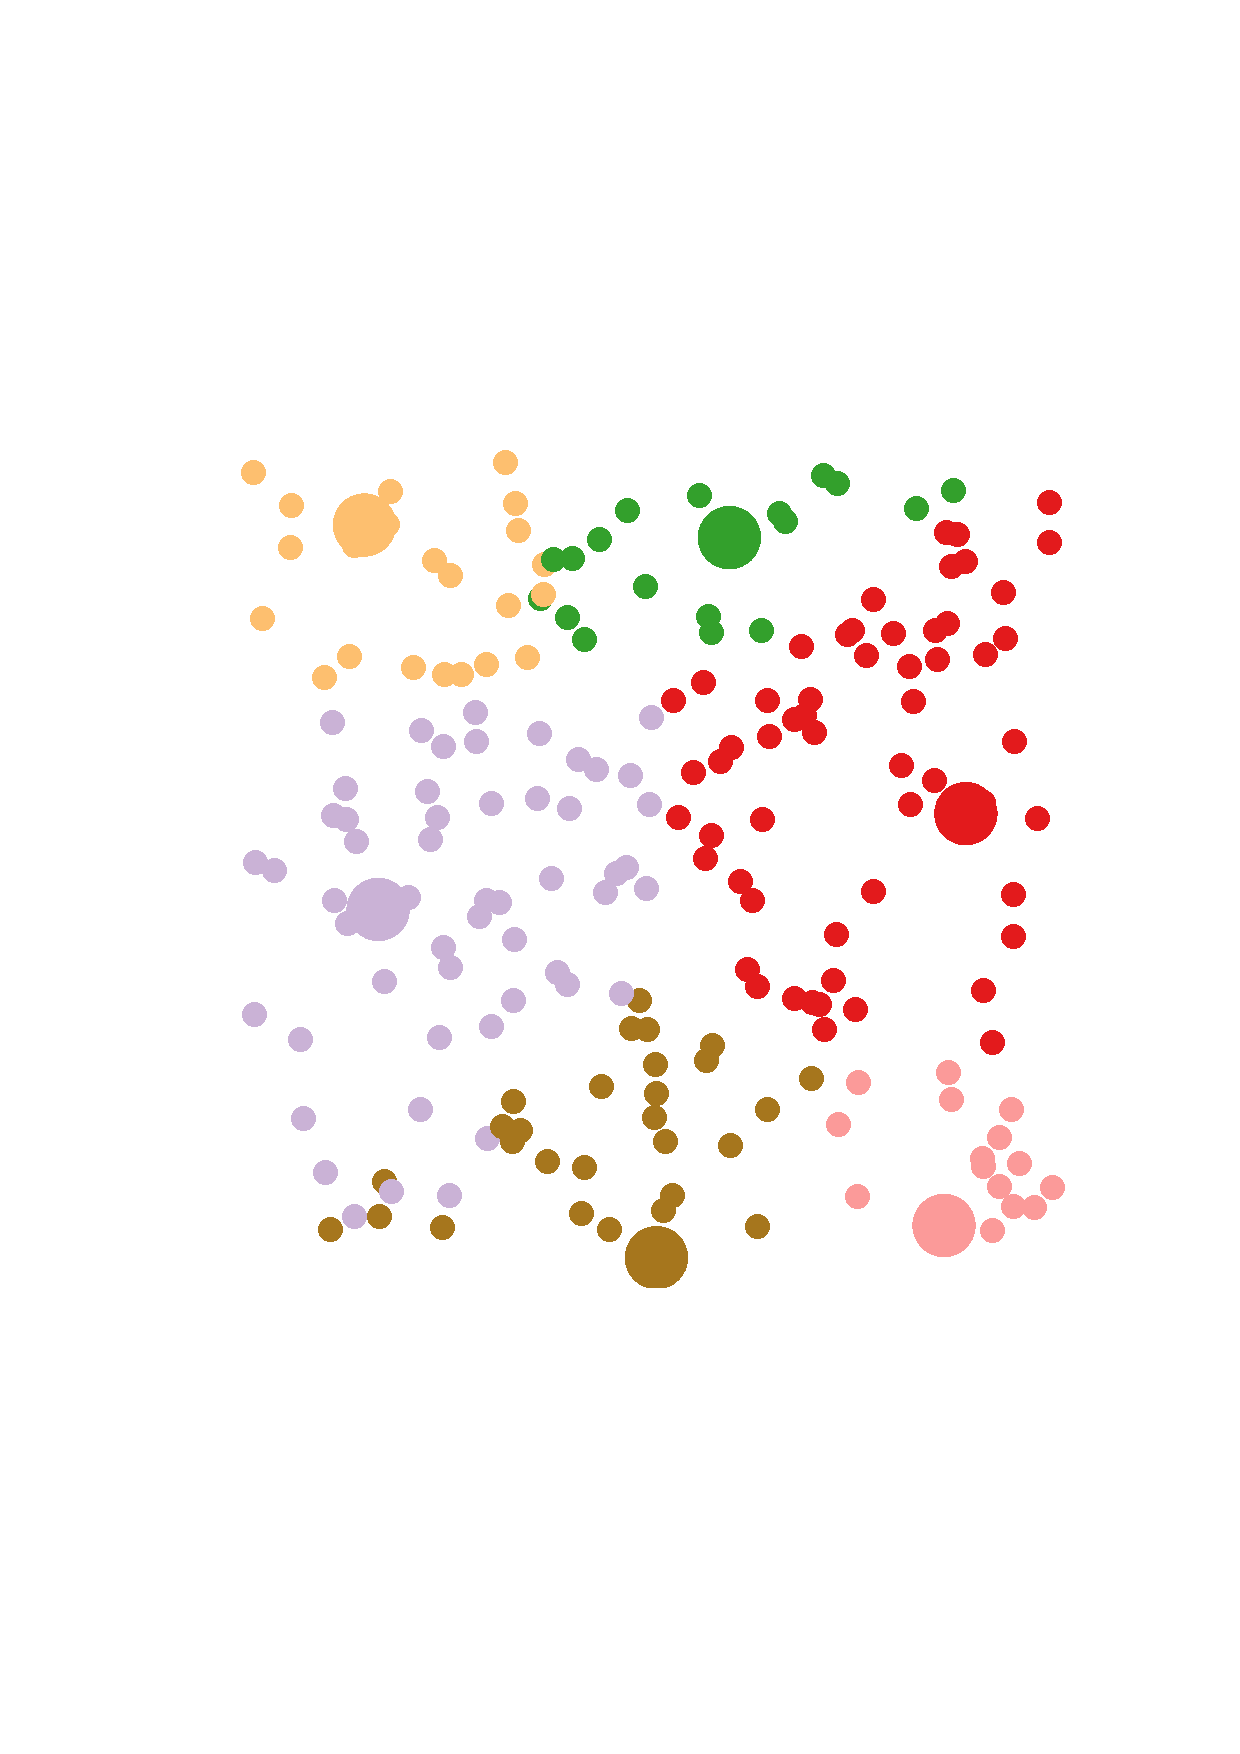
\includegraphics[width=0.7\linewidth]{figure/auxiliary/Frontpage-200-run1-1300x1300.pdf}
\end{figure}

% Cover text
\mbox{}
\vfill
\renewcommand{\familydefault}{\sfdefault} \normalfont % Set cover page font
\textbf{{\Huge 	\headline 	\\[0.2cm] 
				}} 	\\[0.5cm]
{\Large \subtitle}\\[0.5cm]
Master's thesis in Computer Systems and Networks \setlength{\parskip}{1cm}

{\Large \firstauthor} \setlength{\parskip}{2.9cm}\\
{\Large \secondauthor} \setlength{\parskip}{2.9cm}

Department of Computer Science and Engineering \\
\textsc{Chalmers University of Technology} \\
\textsc{University of Gothenburg} \\
Gothenburg, Sweden 2018

\renewcommand{\familydefault}{\rmdefault} \normalfont % Reset standard font
\end{titlepage}


% BACK OF COVER PAGE (BLANK PAGE)
\newpage
\restoregeometry
\thispagestyle{empty}
\mbox{}



% TITLE PAGE
\newpage
\thispagestyle{empty}
\begin{center}
	\textsc{\large Master's thesis 2018}\\[4cm]		% Report number is currently not in use
	\textbf{\Large \headline} \\[1cm]
	{\large \subtitle}\\[1cm]
	{\large \authors}
	
	\vfill	
	% Logotype on titlepage	
	\begin{figure}[H]
	\centering
	% Remove the following line to remove the titlepage logotype
	
\includegraphics[width=0.4\pdfpagewidth]{figure/auxiliary/logo_ch_gu.pdf}
	%
\includegraphics[width=0.2\pdfpagewidth]{figure/auxiliary/logo_eng.pdf}
	\end{figure}	\vspace{5mm}	
	
	Department of \department\\
	%\emph{Division of Division name}\\
	%Name of research group (if applicable)\\
	\textsc{Chalmers University of Technology} \\
	\textsc{University of Gothenburg} \\
	Gothenburg, Sweden 2018 \\
\end{center}


% IMPRINT PAGE (BACK OF TITLE PAGE)
\newpage
\thispagestyle{plain}
\vspace*{4.5cm}
\headline \\
\subtitle\\
\authors \setlength{\parskip}{1cm}

\copyright ~ \firstauthor, 2018. \setlength{\parskip}{1cm}\\
\copyright ~ \secondauthor, 2018. \setlength{\parskip}{1cm}

Supervisor: Olaf Landsiedel, \department\\
Examiner: Marina Papatriantafilou, \department \setlength{\parskip}{1cm}

Master's Thesis 2018\\	% Report number currently not in use 
Department of \department\\
%Division of Division name\\
%Name of research group (if applicable)\\
Chalmers University of Technology and University of Gothenburg\\
SE-412 96 Gothenburg\\
Telephone +46 31 772 1000 \setlength{\parskip}{0.5cm}

\vfill
% Caption for cover page figure if used, possibly with reference to further information in the report
Cover: An example of a clustering of a network with 200 nodes. \setlength{\parskip}{0.5cm}

Typeset in \LaTeX \\
%Printed by [Name of printing company]\\
Gothenburg, Sweden 2018



% ABSTRACT
\newpage
\headline\\
\subtitle\\
\authors\\
Department of \department\\
Chalmers University of Technology and University of Gothenburg\setlength{\parskip}{0.5cm}

\thispagestyle{plain}            % Suppress header 
\setlength{\parskip}{0pt plus 1.0pt}
\section*{Abstract}

Wireless Sensor Networks are becoming more and more popular with the decrease in cost to manufacture sensor nodes and the increased popularity of cyber-physical systems. One of the most significant challenges for Wireless Sensor Networks is to minimise the energy consumption of the nodes, as their battery capacity is often limited, and they are expected to work without human intervention for several years at a time. Another challenge for Wireless Sensor Networks is scalability since they may scale to thousands of nodes. Clustering is a widely used technique to both decrease energy consumption and increase scalability. In this thesis, we aim to increase the network lifetime and the scalability of the \atwo{} system, by integrating clustering with it. Our starting point, \atwo{}, is a system which brings distributed consensus to multi-hop networks implemented on ContikiOS. Our work consists of designing and implementing a clustering scheme, based on the HEED clustering algorithm, to partition the network and create a hierarchical communication medium. We evaluate our work in the Cooja simulator and on the Flocklab testbed, and compare it to the original implementation of \atwo{} using the metrics stability, reliability, latency, and energy usage. Our evaluation shows that we achieve similar reliability to the \atwo{} system but lower stability. However, for the largest network we evaluated, with 200 nodes, we achieve both better latency and lower energy consumption.

% KEYWORDS (MAXIMUM 10 WORDS)
\vfill
Keywords: Wireless Sensor Networks, Scalability, Clustering, HEED, Chaos, \atwo{} Synchrotron

\newpage                % Create empty back of side
\thispagestyle{empty}
\mbox{}

% ACKNOWLEDGEMENTS
\newpage
% CREATED BY DAVID FRISK, 2016
\thispagestyle{plain}			% Supress header
\section*{Acknowledgements}
We would like to thank our supervisor Olaf Landsiedel for his invaluable support and continuous feedback during the project.
%Here, you can say thank you to your supervisor(s), company advisors and other people that supported you during your project.

\vspace{1.5cm}
\hfill
\firstauthor\ \& \secondauthor, Gothenburg, June 2018

\newpage				% Create empty back of side
\thispagestyle{empty}
\mbox{}


% TABLE OF CONTENTS
\newpage
%\Addlcwords{is for an of in the}
\tableofcontents
\iffalse
%CAPS FOR CHAPTER HEADERS
\renewcommand{\chapter}[2][\relax]{%
    \ifx\relax#1%
    %\texorpdfstring FIXES LATEX WARNING. PROBLEM: PDF BOOKMARKS ARE NOT CAPITALIZED
    \svchapter{\texorpdfstring{\titlecap{#2}}{#2}}%
    \else%
    \svchapter[\texorpdfstring{\titlecap{#1}}{#1}]{\texorpdfstring{\titlecap{#2}}{#2}}%
    \fi%
}

%CAPS FOR SECTION HEADERS
\renewcommand{\section}[2][\relax]{%
    \ifx\relax#1%
    \svsection{\texorpdfstring{\titlecap{#2}}{#2}}%
    \else%
    \svsection[\texorpdfstring{\titlecap{#1}}{#1}]{\texorpdfstring{\titlecap{#2}}{#2}}%
    \fi%
}   
\renewcommand{\subsection}[2][\relax]{%
    \ifx\relax#1%
    \svsubsection{\texorpdfstring{\titlecap{#2}}{#2}}%
    \else%
    \svsubsection[\texorpdfstring{\titlecap{#1}}{#1}]{\texorpdfstring{\titlecap{#2}}{#2}}%
    \fi%
}   
\renewcommand{\subsubsection}[2][\relax]{%
    \ifx\relax#1%
    \svsubsubsection{\texorpdfstring{\titlecap{#2}}{#2}}%
    \else%
    \svsubsubsection[\texorpdfstring{\titlecap{#1}}{#1}]{\texorpdfstring{\titlecap{#2}}{#2}}%
    \fi%
} 
\fi
\makeatletter
\xpatchcmd{\paragraph}{3.25ex \@plus1ex \@minus.2ex}{3pt plus 1pt minus 1pt}{\typeout{success!}}{\typeout{failure!}}
\makeatother

% OTHER FRONTMATTER
% List of figures (add to table of contents)
\cleardoublepage
\phantomsection
\addcontentsline{toc}{chapter}{\listfigurename} 
\listoffigures
% List of tables (add to table of contents)
\cleardoublepage
\phantomsection
\addcontentsline{toc}{chapter}{\listtablename}  
\listoftables
\cleardoublepage
\phantomsection
\addcontentsline{toc}{chapter}{\listalgorithmname}
\listofalgorithms


% START OF MAIN DOCUMENT
\cleardoublepage
\setcounter{page}{1}
\pagenumbering{arabic}			% Arabic numbering starting from 1 (one)
\setlength{\parskip}{8 pt plus 1pt}

% INTRODUCTION
\chapter{Introduction}
The technology of Wireless Sensor Networks (WSNs) is an active research area \cite{Yick2008-wsn-survey, Mahmood2015-reliability-survey}, it is a technique that enables small low-powered computer nodes to work in cooperation. The first application of Wireless Sensor Networks was for different military applications such as target tracking and troop movements \cite{Yick2008-wsn-survey}. However, WSNs have quickly expanded to many different fields, such as medical equipment, tracking natural disasters, and monitoring the weather. The nodes are battery powered, with limited processing and storage capabilities. Equipped with a low-power radio, they can communicate with other nearby nodes. They also use sensors to collect data which is then input into some computation and forwarded to a base station or disseminated throughout the network.

One advantage of WSNs is the ability to deploy nodes in the network in an ad hoc manner. Furthermore, the nodes' low powered nature make them inexpensive to manufacture. However, there are multiple challenges which require thorough consideration when implementing protocols for a WSN \cite{Yick2008-wsn-survey}. Since nodes are battery powered, they should restrict the time they spend sending, receiving and processing data to save energy. Another difficulty is maintaining high message propagation speed while not flooding the network with too many messages, hindering propagation of other messages. Additionally, scaling is a challenge; restrictions on the number of nodes in a WSN appear in many forms. For example, due to the maximum size of the transmitted packet, the message distribution algorithm, and node placement since a high node density can constrain message propagation.

The Chaos protocol \cite{chaos-introduction-paper}, presented in 2013, was the first protocol built for WSNs to have native support for all-to-all data sharing. Chaos builds on two core mechanisms. First, synchronous transmissions which means that the nodes in a network follow a global schedule that tells them when to wake up and either transmit or receive data. Second, user-defined merge operators which consist of some code that defines how the node processes and merges the data it receives. For example, calculating the maximum over a set of proposed values. Using these two mechanisms a node running the Chaos protocol can independently decide what action to perform in the next slot (sending data, receiving data, or doing nothing). Additionally, all processing (the execution of a merge operator) is part of the network protocol, just after a node transmits or receives data.

Further development of the Chaos protocol resulted in \atwo{} \cite{a2-introduction-paper}. \atwo{} addressed some shortcomings of the Chaos protocol and also introduced the \atwo{} \textit{Synchrotron}, a synchronous transmission kernel which has several features: frequency hopping, high precision time synchronisation, and the ability to schedule multiple applications to run in the network at different intervals. On top of Synchrotron, \atwo{} implements distributed consensus protocols such as two- and three-phase commit. Due to the new communication model in Chaos and the new features in the \atwo{} protocol, both Chaos and \atwo{} showed significant improvement in performance and reliability compared to similar protocols \cite{chaos-introduction-paper, a2-introduction-paper}.

A typical way to improve the network lifetime and reliability in WSNs is to use clustering \cite{Afsar2014-clustering-survey, Younis2006-clustering-survey}. Clustering is the practice of electing some set of nodes as \emph{Cluster Heads}(CH) and assigning each remaining node to one of these CHs. Nodes selecting a common CH belong to the same cluster and will primarily communicate with that subset of the network. The benefit of clustering is primarily in two different areas. First, since each CH only has to communicate with a subset of the network the amount of data the WSN needs to handle arguably becomes smaller by a factor approximately equal to the number of CHs in the network; however, there is added overhead for clustering the network and communication between CHs. Second, the CHs can aggregate and filter out redundant data from their clusters. This can be beneficial since a common task for a WSN is to forward all data it gathers to a base station. If only the CHs aggregate and forward the data to the base station, the network as a whole can save energy. 

There are many ways of applying clustering in a WSN; they differ primarily in the way the scheme decides the set of CHs. We provide a comprehensive categorisation of different clustering schemes in \cref{sec:background:clustering}.


\section{Limitations}
We impose several limits on the design and implementation of our clustering algorithm. We will not design a new clustering algorithm specifically for the \atwo{} protocol. We will consider an existing clustering algorithm and only make minor modifications to it to make the algorithm work on top of the \atwo{} protocol. Furthermore, we will only provide a basic reference implementation of the clustering algorithm using the \atwo{} Synchrotron as a base.

 \section{Purpose}
The purpose of this thesis is to investigate the effects of exchanging the current all-to-all protocol used in \atwo{} with a protocol based on clustering. The goal is to save energy and make the transfer of information more efficient when compared to the original \atwo{} protocol. We implement a clustering algorithm with modifications to fit \atwo{}s architecture. We also evaluate our implementation and compare it to \atwo{} to see if there is any difference concerning energy usage, latency, and reliability.

\section{Contributions}
Below, we present a brief summary of our main contributions.

\begin{itemize}
    \item We design a clustering scheme for the \atwo{} protocol, based on the HEED algorithm.
    \item We provide a reference implementation of the clustering scheme.
    \item We evaluate our reference implementation in a simulator and on the Flocklab testbed.
\end{itemize}

\section{Outline}
We organise this thesis as follows. In \cref{chap:background} we introduce relevant background about WSNs, the Chaos and \atwo{} protocols as well as clustering. In \cref{chap:related-research} we present research on clustering and communication protocols in WSNs. Following that, in \cref{chap:design} we present our design of the clustering implemented on top of \atwo{}. Next, in \cref{chap:implementation} we talk about the implementation specific details and issues encountered while implementing clustering on top of \atwo{} in Contiki. We present our evaluation of the clustering algorithm and comparison to the existing \atwo{} protocol in \cref{chap:evaluation}. Finally, we conclude in \cref{chap:conclusion}.


% THEORY
\chapter{Background}

\label{chap:background}
In this chapter, we introduce the concept of Wireless Sensor Networks. Moreover, we describe the Chaos and \atwo{} protocol in detail. Finally, we explain what clustering is and provide some insight into different objectives when applying clustering to a network, and also present clustering properties and their categories.


\section{Wireless Sensor Networks}
A \emph{Wireless Sensor Networks} (WSN) consists of many low powered nodes (small computers) equipped with sensors, cooperatively working towards the same goal. Typical applications are within the military for tracking targets, monitoring the weather, and tracking natural disasters \cite{Yick2008-wsn-survey}. A typical node in a sensor network consists of four hardware units for sensing, processing, transmitting and receiving data, and power \cite{Akyildiz2002-wsn-survey}, there can also be additional units for generating power or sensing the location of the node. There are several characteristics of a WSN that while introducing challenges when working with them also are at the core of what makes them useful. Examples of these characteristics are the low power nature of the nodes and ad hoc deployment of the nodes.


One of the primary objectives of a node in a WSN is to preserve as much battery power as possible. Therefore the hardware is often limited in its capabilities, limiting both the radio communication range and the processing power \cite{NikolaosA.Pantaziz2007-wsn-power-survey}. An example of a node called TMote Sky \cite{tmotesky-datasheet}, which we use in this thesis, has a CPU of 8MHz, 10KB RAM, and 48KB of flash storage. The lifetime of the network can be measured in several different ways; one common way is to measure the time until the first node death occurs.

Another focus for the protocol a WSN is running is reliability. The network has to be able to handle a variety of failures such as: packet loss due to interference or transmission error, and nodes failing due to loss of battery power or other unforeseen errors \cite{Mahmood2015-reliability-survey}. In addition, if the network is multi-hop and nodes have to act as forwarders that can introduce several points of failure for a packet before it reaches its intended destination. There exist two primary categories of protocols when talking about how they handle reliability: retransmission and redundancy \cite{Mahmood2015-reliability-survey}. A protocol based on retransmission will have each node wait for acknowledgement of the packet it sends; otherwise, the node will retransmit the packet. A protocol based on redundancy, on the other hand, includes redundancy in the packet itself and will try to correct any faulty bits in any packets received.



\section{Chaos}
The Chaos protocol is the first protocol developed for WSNs that support native all-to-all communication without sequential phases for collection, processing, and dissemination of information \cite{chaos-introduction-paper}. Traditionally, every node in the network had to schedule these phases at the same time, even if some nodes did not have any information to process. In Chaos, every node can take independent decisions on what action to perform (send or receive data), but every node does their respective action at the same time, this is called synchronous transmissions.


The smallest time component in the Chaos protocol is called a \textit{slot}. During a slot, every node performs one of two actions: broadcast or listen for data. At the end of a slot, every node decides what their action will be in the next slot.
A node will broadcast in the subsequent slot if it receives a packet with less or more information than itself. In the first case, it tries to spread its information to the node which sent a packet with less information. In the other case, a node which has just received a packet which contains new information will merge this with their local data and then broadcast the new merged information in the next slot. If a node was listening, but either did not receive a packet or did not gain new information, or if it was broadcasting, then it will listen in the next slot. The next greater time component in Chaos is a series of many slots, and together they are called a round.

During one \textit{round} Chaos executes one application. For example, the max application in which all nodes spread their id across the network and the merge operator (the max application) executed on packet reception returns the maximum between the received number and a nodes local state. The number of slots in a round depends on the network size; a larger network requires more slots than a small network. We give an example of three nodes executing a round in  \cref{fig:chaos-overview}.

\begin{figure}[bt]
    \centering
    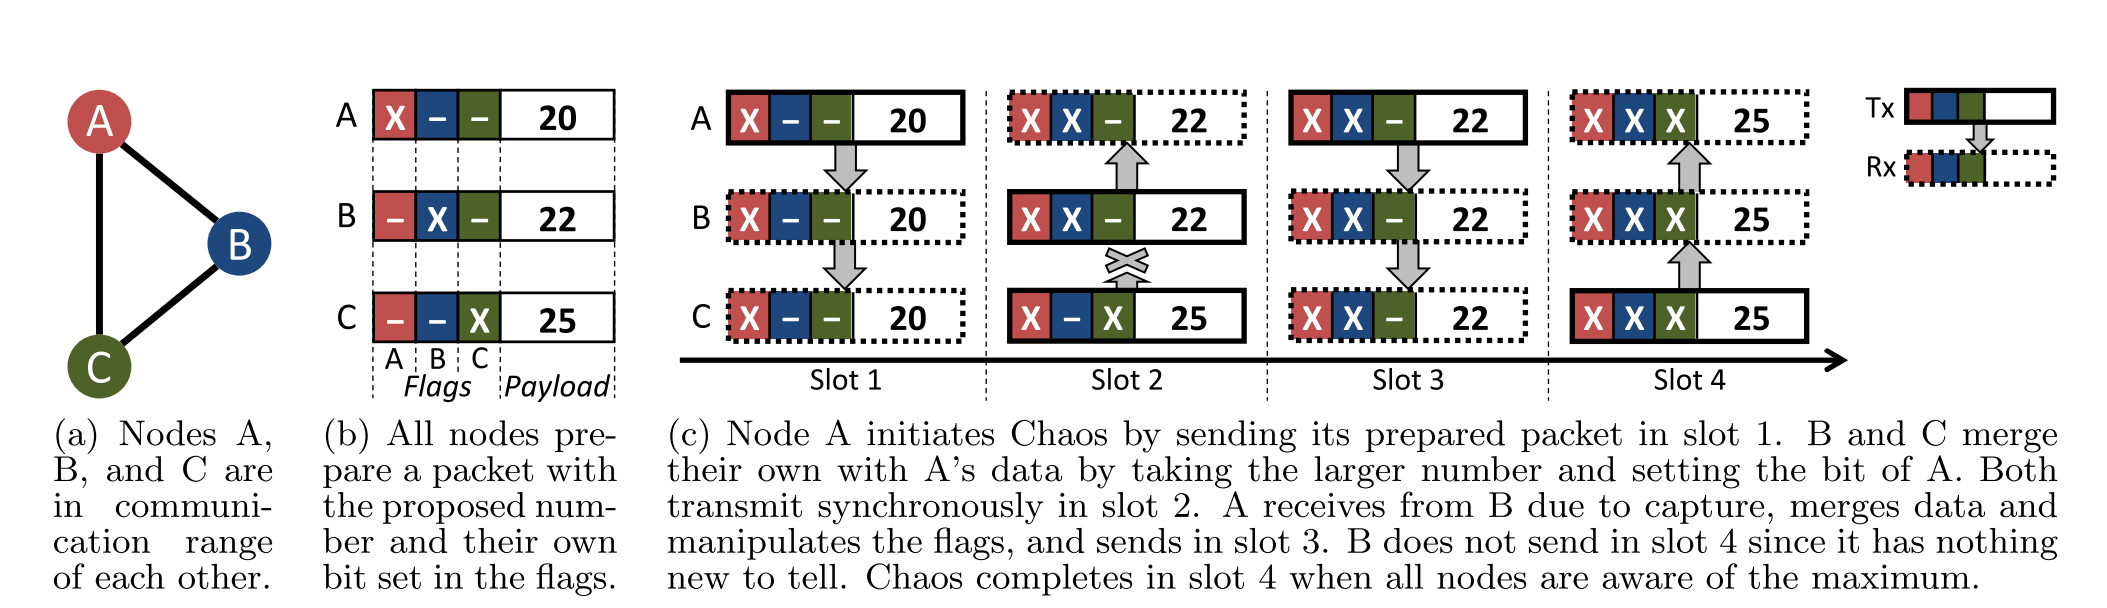
\includegraphics[width=\textwidth]{figure/ChaosOverview.png}
    \caption{Overview of a round in Chaos were three nodes try to reach consensus on a proposed value \cite{chaos-introduction-paper}.}
    \label{fig:chaos-overview}
\end{figure}

\subsection{Synchronous Transmission}
Using synchronous transmissions means that all nodes execute rounds and slots at the same time. In \cref{fig:chaos-overview} time progresses towards the right, and we see that all slots are aligned. This transmission scheme enables Chaos to benefit from two physical phenomena:

\paragraph*{The capture effect} is a physical phenomenon that occurs when packets are colliding (received at the same time by one node). If one signal is sufficiently stronger or the timing between the packets are within a certain threshold, a node will correctly decode the stronger signal, and ignore the weaker one \cite{Lee2007-capture-effect}. Due to this effect, if a node receives two transmissions at the same time, one of them will with a high probability be decoded correctly.

\paragraph*{Constructive Interference} is another physical phenomenon that occurs when multiple nodes are transmitting the same packet at the same time. If that happens, the radio signals get boosted increasing the probability that the packet will be received correctly by another node.

\subsection{The Initiator}
In every Chaos network a special node called \emph{the initiator} needs to be present, node \textit{A} in \cref{fig:chaos-overview}. First, the initiator is the node which initiates communication in a round. It also determines parameters such as what application to run and timing parameters for slots and rounds. All other nodes exclusively listen for packets until one is received which propagated from the initiator, this process is called association. A node will enter association when it boots up and if it does not receive a valid packet for a number of rounds that can be configured depending on the application that is running in the network. The initiator is a predetermined node.

\subsection{Flags Field}
\label{subsec-flags-field}
The \textit{flags field} is a list of boolean values. The field is marked as \textit{flags} in \cref{fig:chaos-overview}. Each node in the network corresponds to an index in the list. At the start of a round, the initiator only sets the value at its index to true. As packets propagate through the network, nodes set the value of their indices to true. Once a node has merged a received packet which sets all values in the flags field to true it knows that all nodes in the network have participated and the information it has is complete. The Chaos protocol has a limitation to its scalability due to the flags field. Since every node requires at least a 1-bit space in the flags field, if there is an upper limit on the packet size imposed by either the link-layer protocol or the sensor nodes, the number of nodes in the network is limited by the maximum size of the packet. 

\subsection{Completion Flooding} % The chaos papers call it the completion policy, they also have the propagation policy as "normal" mode
\emph{Completion flooding} is the last phase of a round. A node enters this phase as soon as all values in their flags field are set to true. Once in this phase, the node broadcasts its completed packet every other slot for a number of slots. Aggressively transmitting the packet causes neighbouring nodes to reach completion which in turn causes them to flood the network with a completed packet. Since all nodes in this phase broadcast the same packet the signal benefits from constructive interference which in turn makes the signal of the complete packet stronger causing the capture effect to apply more often.

\subsection{Timeout Mechanism}
To prevent early termination a \textit{timeout mechanism} triggers if a node has not received any packet for some number of slots. Early termination is when, at the end of a round, some nodes do not have all information. The number of slots is selected randomly by each node from an interval ([3-7] in \cite{chaos-introduction-paper}) causing one or a couple of nodes to broadcast a packet. If nearby nodes have non-equal flag fields, they will continue the packet propagation, and thus communication is reinitiated.

\section{\atwo{} Synchrotron}
\label{sec:chaos-a2-background}
As the original implementation of Chaos has lots of potential, further research conducted by Al Nahas et al.~\cite{a2-introduction-paper} resulted in the Agreement in the Air (\atwo{}) Synchrotron.
As seen in \cref{fig:original-a2-architecture}, \atwo{} is a layer on top of Synchrotron, which is a further development of Chaos. Synchrotron's most prominent features and the ones described here include a dynamic scheduler, parallel channels and channel hopping. From \atwo{} we describe the join and leave services. The remaining architecture description shown in \cref{fig:original-a2-architecture} is explained in \cite{a2-introduction-paper}.

\begin{figure}[bt]
    \centering
    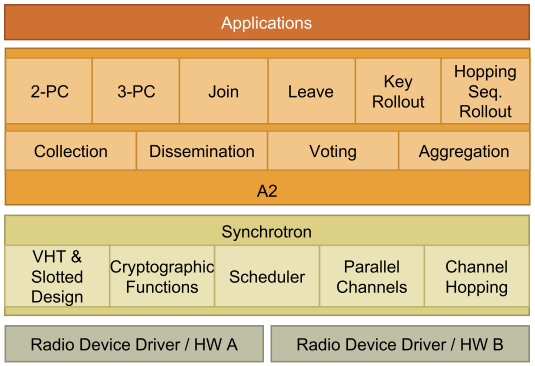
\includegraphics[scale=0.7]{figure/original-architechture.png}
    \caption{The original \atwo{} architecture \cite{a2-introduction-paper}.}
    \label{fig:original-a2-architecture}
\end{figure}

The second contribution is a voting primitive which is used to implement distributed consensus algorithms and a consistent group membership service. 

(include an example of how A2 runs, dynamic join service then application)

\subsection{The Scheduler}
The scheduler in \atwo{} allows the initiator to schedule different applications dynamically. During each round, the initiator sets a \textit{next app} field in the packet to instruct the rest of the network which app should run in the next round.

\subsection{Dynamic Group Membership}
\label{background-a2-join-service}
The join service allows the network to add nodes to the flags field dynamically. A node wanting to join the network sets the join flag in the packet header. Once the initiator receives a packet with a set join flag, it will, during the next round, spread the scheduling of a join round for the subsequent round. The join round then runs in two phases, collect and disseminate. We show an example of the join process with three nodes in \cref{fig:join-service-overview}.

\begin{figure}[bt]
    \centering
    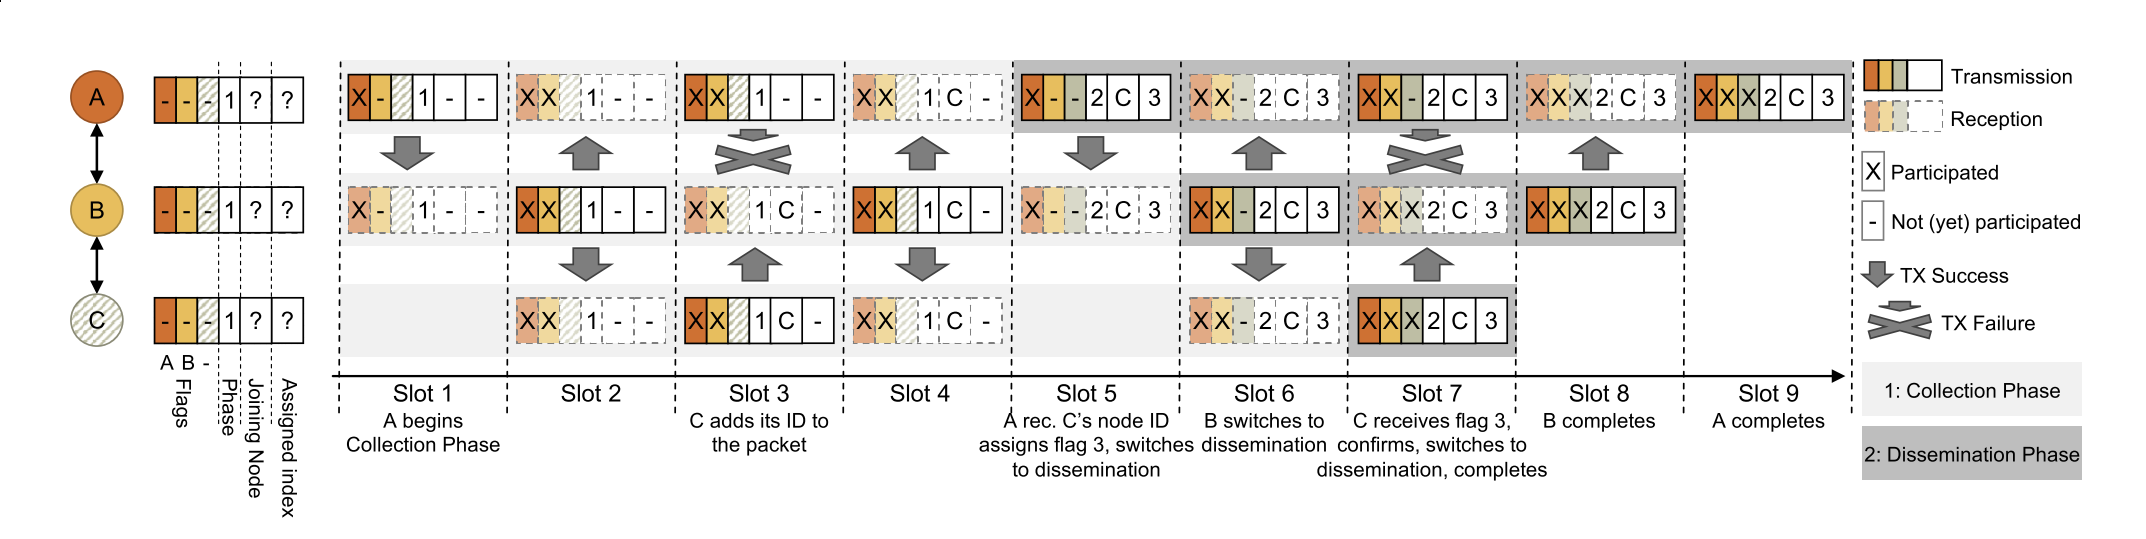
\includegraphics[width=\textwidth]{figure/JoinServiceOverview.png}
    \caption{The join service protocol exemplified using three nodes \cite{a2-introduction-paper}.}
    \label{fig:join-service-overview}
\end{figure}

\paragraph*{The Collect Phase} is the first phase where the network spreads a list in which nodes that want to join the network adds their node ID; this join list is the only way non-joined nodes may contribute to the payload. The initiator will switch to the next phase (Slot 4-5 in \cref{fig:join-service-overview}) when it notices full participation of the network and does not record any changes to the join list for a couple of slots or if the list is full.

\paragraph*{The Disseminate Phase} is the second phase where the initiator assigns each new node an index in the flag field. The initiator then disseminates the join list with updated information about the joining nodes flag indices. Each joining node can now set the flag in their specified index as an acknowledgement (C sets its flag in Slot 7). In case a node misses the dissemination it will requests another join round and be assigned the same flag index again.

The leave service is a rule that the initiator will drop any nodes which it has not seen participation from for a couple of rounds. When the rule triggers, a join round is scheduled to disseminate the information about what nodes are present. The leave service ensures that disappearing nodes does not hinder the completion phase for more than a small number of rounds.

\subsection{Frequency Agility}
\label{subsec-frequency-agility}
In the presence of interference, the performance of \atwo{} degrades. Al Nahas et al.~solves this in Synchrotron by introducing frequency hopping and parallel channels.

\paragraph*{Frequency hopping} in Chaos consists of each node switching which radio channel they use to transmit and receive data in unison in every slot. By switching channels, using the default hopping sequence from the IEEE 802.15.4e standard \cite{IEEE-802-15-4}, the network avoids interference from other traffic, which might occupy a single channel, allowing \atwo{} to exists side-by-side other wireless systems. 

\paragraph*{Parallel Channels} alleviates the issues caused by having a dense network with many nodes transmitting simultaneously in the same area. This causes interference which damages the probability of packet capture. Synchrotron allows for configuring a number of channels from which nodes pick randomly in each slot to use for reception or transmission. The number of parallel channels require configuration and could damage the performance of a network if it is set to high or low. An alternative to parallel channels, proposed by Landsiedel et al., is to reduce the transmission power which would also reduce network density.


\section{Clustering}
\label{sec:background:clustering}

In this section, we cover the topic of clustering. We begin with a high-level description of what clustering in a WSN means. Next, we describe the objectives desired when clustering a WSN. Finally, we describe categories for clustering properties as well as explain the properties that are important for understanding our work.

\subsection{High-level Description}
Clustering is the task of partitioning a network and electing particular nodes, called Cluster Heads (CH), responsible for a network-wide communication overlay \cite{Younis2006-clustering-survey}. All other nodes only communicate within their part of the partition, i.e., their cluster. Each cluster contains one CH which retains all information from the cluster. A typical use case is that all sensor nodes collect data and sends it to a \textit{base station}. A base station is not a sensor node, for example, it is not battery powered and only collects data from other nodes. In some networks, there is no base station; the aim is instead to inform all nodes in the network of the calculated values. In either case, it is the job of the CH to make sure that the relevant parties get the final value.

Related to base stations is the hot spot problem which is a phenomenon that can occur when nodes or cluster heads are using a many-to-one communication pattern \cite{Perillo2005-hot-spot-survey}. Nodes that are closer to the base station will need to handle more routing of traffic, and this can lead to them depleting their energy earlier than other nodes in the network. In the worst case, this can cause the network to become cut off from the base station entirely, completely disabling the network.

Clustering can be beneficial in several aspects; we list some objectives of clustering in \cref{sec:clustering-objectives}. One of the most critical components of a WSN is its energy consumption and using the radio to transmit and receive data is generally the most expensive operation of a node \cite{Anastasi2009-wsn-energy-consumption}. Clustering has been shown to decrease the energy consumption, making clustering an excellent candidate to preserve energy in a WSN.



\section{Clustering Objectives}
\label{sec:clustering-objectives}
There are two categories of clustering objectives, primary and secondary. When designing a clustering algorithm achieving one or more of the primary objectives is often the goal. In contrast, the secondary objectives are usually not of substantial importance for the network, but instead indirectly achieved when clustering the network \cite{Afsar2014-clustering-survey}. We list some primary and secondary objectives in \cref{table:clustering-objective}.

\begin{table}[bt]
\centering
\caption{An overview of primary and secondary clustering objectives \cite{Afsar2014-clustering-survey}.}
\label{table:clustering-objective}
\begin{tabular}{cc}
\multicolumn{2}{c}{{\textbf{Clustering Objectives}}}                   \\ \hline
\multicolumn{1}{c|}{\textbf{Primary}}            & \textbf{Secondary}      \\ \hline
\multicolumn{1}{c|}{Scalability}                 & Increased connectivity  \\
\multicolumn{1}{c|}{Fault-tolerance}             & Reduced routing delay   \\
\multicolumn{1}{c|}{Data aggregation/fusion}     & Collision avoidance     \\
\multicolumn{1}{c|}{Load balancing}              & Using sleep schemes \\
\multicolumn{1}{c|}{Stabilised network topology} &                         \\
\multicolumn{1}{c|}{Maximal network lifetime}    &                        
\end{tabular}
\end{table}

\subsection{Primary Clustering Objectives}
All the primary objectives are usually desired when implementing a clustering algorithm. However, it can be difficult to achieve all of them at the same time. Instead, it is common to target only a few of them.

\paragraph*{Scalability} is a consequence of clustering since the network is partitioned, making the network artificially less dense. Factors which we need to consider when designing for scalability include network density and routing delays.

\paragraph*{Fault tolerance} is common for mission-critical applications. A clustering algorithm can be fault tolerant by periodically reclustering the network. If a node dies and some part of the network loses connectivity, a reclustering can reconnect the network again.

\paragraph*{Data aggregation/fusion} is the act of filtering out redundant data at some earlier point. If the application of a WSN is running is only interested in some average or otherwise redundant data is sent the CH can filter out this data and decrease the number of packets transmitted. Clustering is known to reduce the total network load \cite{Afsar2014-clustering-survey}.

\paragraph*{Load balancing} is achieved by periodically changing the nodes that are CHs. Assuming that being a CH requires more battery, this will increase the total lifetime of the network when clustering is applied.

\paragraph*{Stabilised network topology} concerns the mobility of nodes. If a node moves and switches cluster, the CH can register this change and keep the network topology up to date.

\paragraph*{Maximal network lifetime} is a very common objective often, in part or entirely, caused by the other objectives. For example, proper load balancing means avoiding early node deaths, and data aggregation mean the network can send fewer packets. Both of these properties work towards an energy efficient cluster which implies a more extended network lifetime. 

\subsection{Secondary Clustering Objectives}
The secondary objectives are not usually a target when implementing clustering algorithms but rather achieved indirectly or enabled by them.

\paragraph*{Increased connectivity,} in a clustered network only the CHs needs to be connected to each other. All other nodes only have to be connected to their cluster which makes it easier to make the network fully connected.

\paragraph*{Reduced routing delay,} some applications may require a minimum routing time to perform as intended for example applications recording physical events such as earthquakes. To have a proper quality of service packets need to arrive within a specified time limit. In a widespread WSN, this can be a challenge.

\paragraph*{Collision avoidance,} transmission collisions may cause packet loss which is energy wasted on doing nothing. To minimise packet loss clusters can split their communication between different radio channels or different time slots.

\paragraph*{Using sleep schemes,} in some applications there is no need for the whole network to be active. For example, some nodes might only provide routing paths, in this case, all paths need not always be active. Thus, enable routing to work longer without any node deaths.


\section{Clustering Technology Properties}
\label{subsec:background:clustering-algorithm-categorisation}

There exist several ways of categorising the properties that define clustering algorithms. Afsar et al.~\cite{Afsar2014-clustering-survey} describe three main categories: Cluster properties, Cluster Head properties and Clustering process properties. Here, we summarise each category and list the properties within each of them.

\subsection{Cluster Properties}
The \textit{cluster properties} summarised in \cref{table:cluster-properties} describe properties of the clusters the algorithm creates.

\paragraph*{The size of clusters} in a WSN can either be tailored by the algorithm to be equal or unequal. In an equal clustering algorithm the algorithm will enforce an equal size on all clusters while in an unequal algorithm the clusters will vary in size according to some criteria, for example, distance to a base station; if a cluster is closer to a base station, the cluster size will be smaller.

\paragraph*{The number of clusters} can either be predefined or variable. When the cluster size is variable, it would be due to a probabilistic CH election process.

\paragraph*{The communication distance} can be either \textit{single-hop} or \textit{multi-hop} communication for both \textit{intra-cluster} and \textit{inter-cluster communication}. Inter-cluster requires multi-hop communication when the number of CHs are few and spread out since they will need help with forwarding to reach the other CHs. Intra-cluster communication needs to be multi-hop when there is a bound on the number of CHs since every node might not be able to reach a CH in a single hop.

\begin{table}[bt]
\centering
\caption{Cluster properties and their options.}
\label{table:cluster-properties}
\begin{tabular}{cl}
\multicolumn{2}{c}{\textbf{Cluster Properties}}                                                                         \\ \hline
\multicolumn{1}{c|}{\textbf{Property}}           & \multicolumn{1}{c}{\textbf{Options}}                                 \\ \hline
\multicolumn{1}{c|}{Cluster size}                & \begin{tabular}[c]{@{}l@{}}Equal\\ Unequal\end{tabular}              \\ \hline
\multicolumn{1}{c|}{Cluster count}               & \begin{tabular}[c]{@{}l@{}}Constant (preset)\\ Variable\end{tabular} \\ \hline
\multicolumn{1}{c|}{Intra-cluster communication} & \begin{tabular}[c]{@{}l@{}}Single-hop\\ Multi-hop\end{tabular}       \\ \hline
\multicolumn{1}{c|}{Inter-cluster communication} & \begin{tabular}[c]{@{}l@{}}Single-hop\\ Multi-hop\end{tabular}      
\end{tabular}
\end{table}

\subsection{Cluster Head Properties}
The cluster head properties listed in \cref{table:cluster-head-properties} define different behaviours for the cluster heads.

\paragraph*{The mobility} of a node is either mobile or stable. A mobile CH induces frequent topology changes which add overhead.

\paragraph*{The node type} is either homogeneous or heterogeneous. An algorithm with heterogeneous nodes means a node could have additional resources such as elevated energy reservoir, computing power or transmitting range. Making it more suitable to be CH than other nodes.

\paragraph*{The role} of a CH is either only to relay messages or to both relay messages and perform the same operations regular nodes do, such as collecting and aggregating data.

\begin{table}[bt]
\centering
\caption{Cluster head properties and their options.}
\label{table:cluster-head-properties}
\begin{tabular}{cl}
\multicolumn{2}{c}{\textbf{CH Properties}}                                                                    \\ \hline
\multicolumn{1}{c|}{\textbf{Property}} & \multicolumn{1}{c}{\textbf{Options}}                                  \\ \hline
\multicolumn{1}{c|}{Mobility}          & \begin{tabular}[c]{@{}l@{}}Mobile\\ Stationary\end{tabular}          \\ \hline
\multicolumn{1}{c|}{Node types}        & \begin{tabular}[c]{@{}l@{}}Homogeneous\\ Heterogeneous\end{tabular}  \\ \hline
\multicolumn{1}{c|}{Role}              & \begin{tabular}[c]{@{}l@{}}Relay\\ Aggregation/Fusion\end{tabular}
\end{tabular}
\end{table}

\subsection{Clustering Process Properties}
The clustering process describes the properties used to create the cluster, these properties are often more high level and describe the process as a whole.

\paragraph*{The method} used for clustering can be either distributed or centralised. A distributed algorithm has the potential to create clusters faster since each node can make its own decision. However, a centralised approach can create more optimised clusters since it has a global view of the network.

\paragraph*{CH election} can either be preset, random or attribute based. Preset is when the person who configures the network chooses which nodes are cluster heads during setup. The opposite of a preset approach is a random approach, letting the nodes become cluster heads with a probability. As a middle road, nodes may select CHs with a more complicated process using attributes such as remaining energy or the number of neighbours.


\paragraph*{The algorithm complexity} is either constant or variable. A constant complexity means setup time is not dependent on network size while a variable time algorithm can converge on better choices for cluster heads. 

\paragraph*{The nature} of the clustering process can either be proactive or reactive. Proactive means that it does not consider what application will run on it. In contrast, the process's nature can also be reactive or data-centric meaning it tries to optimise the cluster for a specific application and the data flow required by it.

\paragraph*{The dynamism} of the algorithm can be either dynamic or static. In a dynamic approach, CHs are elected based on the current conditions of the network while a static approach would yield the same result no matter when the algorithm executes.


\begin{table}[bt]
\centering
\caption{Clustering process properties and their options.}
\label{table:clustering-process-properties}
\begin{tabular}{cl}
\multicolumn{2}{c}{\textbf{Clustering Process}}                                                                       \\ \hline
\multicolumn{1}{c|}{\textbf{Property}}    & \multicolumn{1}{c}{\textbf{Options}}                                      \\ \hline
\multicolumn{1}{c|}{Method}               & \begin{tabular}[c]{@{}l@{}}Distributed\\ Centralised\end{tabular}         \\ \hline
\multicolumn{1}{c|}{CH election}          & \begin{tabular}[c]{@{}l@{}}Preset\\ Random\\ Attribute based\end{tabular} \\ \hline
\multicolumn{1}{c|}{Algorithm Complexity} & \begin{tabular}[c]{@{}l@{}}Constant\\ Variable\end{tabular}               \\ \hline
\multicolumn{1}{c|}{Nature}               & \begin{tabular}[c]{@{}l@{}}Proactive\\ Reactive\end{tabular}              \\ \hline
\multicolumn{1}{c|}{Dynamism}             & \begin{tabular}[c]{@{}l@{}}Dynamic\\ Static\end{tabular}                  \\ \hline
\multicolumn{1}{c|}{Objectives}           & See table \ref{table:clustering-objective}                                                       
\end{tabular}
\end{table}

\chapter{Related Research}
\label{chap:related-research}
There is a variety of research on clustering in Wireless Sensor Networks. In this section, we present a few influential clustering protocols such as HEED and LEACH to highlight their key ideas and their similarities and differences. We also present other research which improves the scalability of the Chaos protocol using estimation vectors. Finally, we end with a comparison to our clustering algorithm.

\section{Equal and Unequal Clustering}
\textit{Hybrid Energy-Efficient Distributed Clustering} (HEED) \cite{Younis2004-HEED} is a probabilistic, attribute-based clustering algorithm with the primary objective of saving energy. Unequal HEED (UHEED) \cite{Ever2012-UHEED} builds on HEED and makes the algorithm unequal to solve the hot spot problem. In this section, we first present the internal workings of HEED, followed by the changes introduced by UHEED.

\subsection{HEED}
Younis et al.~present HEED \cite{Younis2004-HEED}, a probabilistic, equal clustering algorithm with the primary objective of saving energy. To this end, HEED uses residual node energy as its main parameter to elect CHs and intra-cluster communication cost as its second parameter. An example of intra-cluster communication cost is the number of nodes that have already joined a cluster. In HEED, the clustering algorithm executes at regular intervals ranging from seconds to hours depending on the application running in the WSN and how significant the increase in energy consumption is when a node is a CH.

At the start of the clustering algorithm, each node sets an initial probability to, for example, $C_{prob} = 5\%$ and then apply its proportion of residual energy as weight according to the following formula to calculate the probability of becoming CH as: $$CH_{prob} = C_{prob} * \frac{E_{residual}}{E_{max}}$$ Where $E_{residual}$ and $E_{max}$ is the residual energy and the maximum possible energy respectively. The value of $CH_{prob}$ is limited by a carefully selected lower bound, inversely proportional to the value of $E_{max}$ to ensure that the algorithm terminates in $\mathcal{O}(1)$ time.

Furthermore, there are two stages for any node announcing itself as CH; a node first becomes a \textit{tentative} CH until it either resigns or becomes a \textit{final} CH. During every iteration of the algorithm, every node will double the value of $CH_{prob}$ until it reaches 1 or the algorithm terminates. A node announces itself as a tentative CH with probability $CH_{prob}$ if it has not heard from any other CH and moves on to become a final CH if $CH_{prob} = 1$. If a node reaches the end of the algorithm without selecting a final CH, it will announce itself as a final CH. Last, a CH will resign from being tentative CH if it finds another CH with lower cost.

\subsection{UHEED}
UHEED \cite{Ever2012-UHEED} builds upon HEED; the most significant change is that UHEED is an unequal clustering algorithm. The algorithm will create smaller clusters when closer to the base station to mitigate the hot spot problem. The idea is that CHs that are closer to the base station will need to handle more routing traffic from other clusters and thus have a higher energy consumption than a CH further away from the base station.

The clusters get progressively smaller by defining a \textit{competition radius} which is the area a node considers when choosing CH. UHEED uses the formula to calculate the competition radius developed by Lie et al.~\cite{Li2005-EEUC}. The formula uses the maximum distance between nodes and the current distance to the base station as parameters. Evaluations of HEED and UHEED showed that UHEED had an equal or better performance in virtually every case when compared to the state of the art \cite{Ever2012-UHEED}.


\section{LEACH}
A significant reactive clustering protocol developed in 2002 is LEACH \cite{Heinzelman2002-leach}. Heinzelman et al.~designed LEACH for applications that measure something in the environment where the interesting results are not the individual values but some computation using those values. The clustering algorithm in LEACH is distributed and probabilistic with the primary objective of saving energy.

The LEACH algorithm divides into rounds. Rounds in Leach is conceptually different to Chaos. Each round begins with a setup phase which forms the clusters, followed by a steady state phase where nodes collect data and CHs aggregate and forward that data to the base station. In the setup phase, each node has a probability $P_i(t)$ at time $t$ to announce themselves as CH. This probability is dependent on a number $k$, which is the target amount of clusters. In a network that contains $N$ nodes, we choose the probability $P_i(t)$ so that the following formula holds.

$$E[\#CH] = \sum_{i=1}^N P_i(t) * 1 = k$$

Also, to maximise network lifetime, each node takes on an equal responsibility of becoming a CH. Thus, if there are $N$ nodes in the network, each node will on average be CH every $N/k$ rounds.

When all nodes have decided if they are a CH, they need to inform the rest of the network of this decision. They do this by sending out an advertisement message containing their ID. All other nodes will listen for these messages and map each CH with the energy required to transmit a packet to it. The node then picks the CH with the lowest transmission energy.

\section{Extreme Chaos}
Chronopoulos \cite{Chronopoulos2016-extreme-chaos} addresses the scaling bound on the number of participating nodes described in \cref{sec:chaos-a2-background}. In particular, Chronopoulos addresses the completion vector which is bounded by the 802.15.4 packet size of 127 bytes \cite{IEEE-802-15-4}. The completion vector in the \atwo{} protocol is the flags field created by the join service as detailed in \cref{subsec-flags-field}. The vector requires only one bit per member, but together with the additional information required in the packet (synchronisation, error-detection and payload), the number of possible participating nodes is less than a thousand \cite{chaos-introduction-paper}. Chronopoulos also discusses how the flags field affects the latency of transmission. They note that increasing the network size by a factor of 10 increases the delay in the network by a factor of 100 \cite{Chronopoulos2016-extreme-chaos}. Last, they note that the completion vector also imposes an overhead on the energy consumption when it is transmitted. Since transmission requires a significant amount of energy, the design of the completion vector is worth restructuring.

\subsection{Estimation Vector}
From the arguments above Chronopoulos reasons that the most significant improvement for the Chaos protocol is to replace the flags field. Hence, they propose an estimation vector which is the most prominent part of the new protocol. Just as the flags field, the estimation vector is used for keeping track of how much of the network has contributed to the aggregate. Chronopoulos argues that extreme values spread quickly throughout the network and therefore nodes do not need to make sure they have communicated with every other node. As such we only need to set a percentage of the flags. However, this does not reduce the size of the flags field. The new vector tries to estimate the number of nodes which has contributed to the aggregate, by also estimating the network size the nodes infer the contribution ratio. 
%The theory used is called a cardinality estimator[source to original paper used in extreme chaos].


%% The procedure of generating and maintaining the estimation vector is a complicated one. Each node begins by generating its starting vector of $n$ values picked from a range $[1-m]$

\subsection{Flow Control}
An additional issue addressed by Chronopoulos is the high number of transmitters at the beginning of a round whom together flood the network. The mechanism put in place to counter this flooding is called flow control, and its purpose is to prevent congestion from occurring by applying an \textit{exponentially decaying back-off probability} \cite{Chronopoulos2016-extreme-chaos}. The back-off is a node deciding, according to some probability, to not send during a slot at which it was originally scheduled to do so. The exponential decay is referring to the probability decreasing at an exponential rate throughout the round. Stopping congestion in early slots will make an aggregate progress quick which enables a round to finish earlier.

To not have adverse effects the parameters used for calculating the next probability for back-off requires careful testing. Having a too low probability of back-off would mean the initial flooding is not constrained enough. In contrast, a too high probability means dropping later transmissions which would hinder the aggregation process. Similarly, flow control can affect large and small networks differently. In a large network, an extended period with initial high flooding can occur. Chronopoulos argues that this is because nodes far from the initiator join the network in later slots. However, Chronopoulos does not consider large networks since their primary focus is to optimise Chaos for local neighbourhoods.

\section{Discussion}
In this thesis, we base our clustering algorithm on the one presented in HEED. However, we make some changes to fit the \atwo{} protocol better but these are mostly regarding specific implementation details. We present these changes in \cref{chap:design} and \cref{chap:implementation}. We do not use any of the modifications presented about UHEED in our implementation since we do not consider base stations.

Furthermore, the LEACH protocol is similar to HEED in that it is also probabilistic; however, its scope is more narrow. It has a dependency on the applications that are running the protocol which we found limiting for our work. Also, the algorithm tries to enforce that every node in the network becomes CH eventually, this is not a desirable property for us since there might be nodes in the network which would be bad CHs.

Lastly, Extreme Chaos is another approach that addresses the scalability issues that Chaos has due to the flags field. However, there is one significant difference. By using an estimation vector rather than the complete flags field there is never a guarantee that the network has reached completion, there will always be some uncertainty. Using clustering instead could give a suboptimal clustering, but there will never be any uncertainty as to if the network has completed or not. Finally, using clustering in a WSN is an explored area with much research behind it. 


% METHODS
\chapter{Design of the Clustering Process}
\label{chap:design}
In this chapter, we explain the design behind our clustering implementation and put its objectives and properties into context. First, we provide an overview of the clustering process. Second, we go into detail about the Clustering service, explain how we design for scalability, and explain the CH election algorithm. Third, we explain of how nodes pick cluster heads from the elected set of CHs. Fourth, we describe a Demote service which runs after the Clustering service to remove suboptimal clusters. Fifth, we explain how communication works between CHs and how clusters avoid interfering with each other's communication. Last, we discuss decisions we make regarding the design and the effect of those decisions.

\section{Clustering Process Overview}
To increase the scalability and lower the energy consumption of \atwo{}, we design and implement a clustering process based on the HEED clustering algorithm \cite{Younis2004-HEED}. The process is responsible for clustering the network, appointing nodes as CHs, and letting nodes join clusters.

Our clustering process consists of four distinct phases. First, the Clustering service runs, and every node does three things simultaneously: While \textit{(i)} learning about the network topology by collecting statistics about received packets, they also \textit{(ii)} try to become CH, and if they hear another node announcing itself as CH within the configured competition radius they \textit{(iii)} select an appropriate cluster to join. Second, each elected CH runs the Join service from \atwo{} inside their cluster. Third, all clusters which deem themselves too small disband, and all nodes in these clusters select other clusters. Fourth, each CH rerun the Join service to determine the final set of nodes in their cluster. This process is repeated at a certain round interval to accommodate for changing battery levels for nodes in the network.

When the clustering process is complete, the network executes some application, in our case, the Max application. At this point, we split the rounds in \atwo{} into \emph{cluster} and \emph{cluster head} rounds. In cluster rounds, each cluster will separately execute an application to completion. In CH rounds, the CHs execute the same application again, but they remember the information they got in the previous cluster round. What that information is, depends on the application; in the Max application's case, it is the maximal value found in each cluster.
The process of alternating between \emph{cluster} and \emph{cluster head} repeats until the clustering process starts again.

\section{The Clustering Service}
The Clustering service is responsible for clustering the network, and it needs to run first to enable a clustered communication medium. In this section, we describe the design of the Clustering service, how we design for scalability, how the clusters are formed, and the parameters that control the Clustering service.


\subsection{Designing for Scalability}
Because our primary goal is to increase the scalability of the \atwo{} system, a challenge is the packet size restriction of 127 bytes, imposed by the 802.4.15 standard \cite{IEEE-802-15-4}. If an application adds data to the packet and if that data grows linearly with the number of nodes in the network, then the application will quickly reach the packet size restriction. Because the flags field is part of all packets and does grow linearly, we want to prevent it from growing too large. Consequently, we need to cluster the network before running the Join service. Therefore, we design the Clustering service to run without completion flags. Running the Join service after the Clustering service puts the scaling restriction of the flags field locally in each cluster. However, the network cannot perform completion flooding or early turnoff during the Clustering service, as completion is calculated from the flags field. Nonetheless, it is vital that all nodes learn of all CHs since nodes use that information to maintain a flags field for CH rounds.

\subsection{Transmission Policy with Gossiping}
Without completion flags, nodes cannot determine when consistency has been reached. Therefore, we inspire the transmission policy of the Clustering service from gossiping protocols, to benefit from the high probability of gossiping to disseminate updates successfully. The transmission policy for the Clustering service is that a node should transmit in the next slot if it received a list that contains a CH which the node did not know about, or the list is missing a CH the node does know about; otherwise a node will try to receive data.


\subsection{Election of Cluster Heads}
The CH election algorithm is based on the HEED algorithm \cite{Younis2004-HEED}, it is probabilistic and attribute based. The Clustering service is executed over several rounds, and the algorithm is divided into two phases: the main phase, shown in \cref{alg:ch-decision}, and the final phase, shown in \cref{alg:ch-final}. The main phase probabilistically elects a set of CHs based on their residual energy, nodes with more residual energy has a higher chance of becoming a CH. In this phase, every node also chooses a cluster to join. The final phase ensures that CHs cover the whole network.

In every round, all nodes have set a probability to announce themselves as CH, and they double that probability at the end of every round until it reaches $1$; at that point, each node has either heard another CH they can join or elected themselves to be CH. The algorithm ensures that a stable set of CHs is elected in constant time \cite{Younis2004-HEED}.

Nodes calculate their initial probability ($CH_{prob}$), to announce itself as CH, according to

\begin{equation}
    CH_{prob} = C_{prob} * \frac{E_{residual}}{E_{max}}
    \label{eq:ch-election-probability}
\end{equation}

taken from HEED \cite{Younis2004-HEED}. $C_{prob}$ is an initial probability which is used to get the process started; it does not have any impact on the final number of cluster heads \cite{Younis2004-HEED}. $E_{residual}$ is the residual energy of the node and $E_{max}$ is the maximum energy of the node. Furthermore, $CH_prob$ is bounded by $p_{min}$, a constant lower bound inversely proportional to $E_{max}$, which ensures that $CH_{prob}$ reaches 1 in constant time.

The number of consecutive Clustering service rounds required to form stable clusters differs between networks. It depends on the network topology, the diameter of the network, and the lower bound on the initial probability. For example, a sparse network requires more rounds than a dense network.

There are two states for a CH in the HEED algorithm: tentative and final. A CH is tentative until its probability of becoming CH reaches 1, then it becomes final. This distinction is made to prune out nodes which have lower residual energy. Since the Clustering service runs for a fixed number of rounds, if a CH is still tentative when the Clustering service begins the final phase and it can find another cluster to join, it will be demoted and join that cluster. 

Furthermore, we control the number of nodes that can become CHs in two ways. As can be seen in \cref{alg:ch-decision} at \cref{alg-heed-valid-clusters-not-empty}, a node is only allowed to announce itself as CH with probability $CH_{prob}$ if either of two things holds. First, taken from HEED, a node must not have seen another CH within their competition radius (measured in hops). Second, further defined by us, a node may still elect itself if the $neighbourRatio$, that is, the number of neighbours divided by the number of CHs within a nodes competition radius, is larger than the parameter \emph{nodes per cluster ratio}. We explain this parameter in more detail in \cref{sec:clustering-parameters}, but its primary purpose is to make dense networks sparser, thus decreasing interference.

However, if two nodes decide to become CH in the same round, then both of them will begin to announce themselves at the start of the next round. This may cause two nodes within each others competition radii to become CHs; to decrease the risk of this, nodes will wait until a random slot during the first half of the next round before they begin to announce themselves. This gives another newly elected CH a chance to hear another nearby CH, which they can join before they announce themselves. We limit this random back off to the first half of a round to ensure that the CHs do not announce themselves too late not to be noticed by other CHs.

\begin{algorithm}[bt]
\caption{The repeat phase adaptation of the HEED algorithm. It shows how a node elects to announce itself as cluster head. The algorithm is adapted for \atwo{} in two ways. We utilise our parameter $nodesPerClusterRatio$ at \cref{alg-heed-valid-clusters-not-empty} and set the announcement slot at \cref{alg-heed-tentativeAnnouncementSlot}.}
\label{alg:ch-decision}
\begin{algorithmic}[1]
%\setcounter{ALC@unique}{0}
\Procedure{heed\_repeat}{}
\If{$prevCH_{prob} \leq 1$}
    \If {$validCHList \neq \emptyset \text{ or } neighbourRatio > nodesPerClusterRatio$} \label{alg-heed-valid-clusters-not-empty}
        \State $myCH \gets pickBestCH(validCHList)$
        \If {$myCH = myNodeID$}
            \If{$CH_{prob} = 1.0$}
                \State $CHState \gets \text{FINAL}$
            \Else
                \State $CHState \gets \text{TENTATIVE}$
            \EndIf
        \EndIf
    \ElsIf {$CH_{prob} = 1$}
        \State $CHState \gets \text{FINAL}$
    \ElsIf {$random(0, 1) \geq CH_{prob}$}
        \State $announcementSlot \gets random(1, maxAnnouncementSlot)$ \label{alg-heed-tentativeAnnouncementSlot}
    \EndIf
    
    \State $prevCH_{prob} \gets CH_{prob}$
    \State $CH_{prob} \gets min(2CH_{prob},1)$
\EndIf
\EndProcedure
\end{algorithmic}
\end{algorithm}

\subsection{The Final Phase}
\label{subsec:final-phase}
HEED's final phase executes during the last three rounds of the Clustering service. It performs two important functions, it demotes tentative CHs and ensures that CHs cover the whole network. We show the pseudo code for the final phase in \cref{alg:ch-final}.

The final phase serves the same purpose in both our algorithm and HEED, but CHs are tentative for different reasons. In HEED, the only reason a CH is tentative in the final phase is if it announced itself as CH and then found another CH with a lower cost to join, according to a cost function. In HEED, the cost function is based on the communication cost between nodes and the CHs \cite{Younis2004-HEED}. However, in our algorithm, a CH is tentative in the final phase if it does not have enough energy to reach a probability of $1.0$ before the final phase begins. Additionally, the final phase ensures that the whole network is covered. As can be seen in \cref{alg:ch-final}, if a node does not consider any CH to be valid, i.e. exist within the competition radius, it will announce itself as CH; this guarantees that cluster heads cover the whole network.



\begin{algorithm}[bt]
\caption{The final phase of the clustering algorithm. The only edit from the original HEED final phase is the usage of $pickBestCH$, which is our definition of the cost function that the HEED algorithm requires.}
\label{alg:ch-final}
\begin{algorithmic}[1]
\Procedure{heed\_final\_phase}{}
    \If{$CHState \neq \text{FINAL}$}
        \If {$CHList \neq \emptyset$}
            \State $myCH \gets pickBestCH(CHList)$
            \State $CHState \gets \text{NOT\_CLUSTER\_HEAD}$
        \Else
            \State $CHState \gets \text{FINAL}$
        \EndIf
    \EndIf
\EndProcedure
\end{algorithmic}
\end{algorithm}

\subsection{Configuration Parameters}
\label{design:configuration-parameters}
In this section, we describe the parameters that change the behaviour of the Clustering service: competition radius, minimum cluster size, and nodes per cluster ratio. We evaluate the effect of changing these parameters for different network topologies in \cref{chap:evaluation}.

\paragraph*{Competition radius,} measured in hop count, is a measurement of how far away a node can be from a CH and still join that CH. In a small and dense network, a small competition radius will make the network less dense by partitioning it into many clusters and thus lowering the number of packet collisions. On the other hand, in a large and sparse network, a high competition radius will keep the number of cluster heads low to ensure that the clusters do not get too small. 


\paragraph*{Minimum cluster size} is the number of nodes, including the CH that has to be a part of the cluster for it to be considered valid. If a cluster has few nodes, one of the three following scenarios is likely to have occurred. First, the network could have been small or sparse, clustering such a network makes it even more sparse which could damage reliability and stability. Second, the CH could be poorly located, for example, close to the edge of the network or far away from other nodes. Third, the CH could be close to another CH that most of the nodes around them chose to join instead. In both the second and the third case our algorithm elected a bad CH which can be pruned relatively easily when the clustering process is complete. In the first scenario, it is hard for small and sparse networks to benefit from clustering.


\paragraph*{Nodes per cluster ratio,} tries to enforce a maximum cluster size to make a dense network artificially sparser. It is not a strict limit on the number of nodes in a cluster. Instead, it is a limit on the number of CHs that can announce themselves depending on the number of neighbours they have. A node with more neighbours than \emph{nodes per cluster ratio} will still be able to announce itself even if it has heard from another CH within its competition radius, dividing the neighbours between itself and other CHs, which makes the network less dense.

%\begin{table}[bt]
%\centering
%\caption{List of configurable parameters for the Clustering service.}
%\label{table:configuration-parameters}
%\begin{tabular}{l}
%\textbf{Parameter name}      \\ \hline
%Competition Radius      \\
%Minimum Cluster Size      \\
%Nodes Per Cluster Ratio
%\end{tabular}
%\end{table}

\section{Joining Clusters}
The primary objective of a node is to choose a cluster head that requires the least cost to join. To do this, we define a function that tries to find the CH that is closest to that node. Since a typical WSN is an ad hoc network, we have to gather information about the network while our Clustering service is running. Each node keeps track of two metrics to estimate how close other nodes are: The number of packets they receive from their neighbours (nodes that can be reached in a single hop) and the number of hops required to reach each CH. A node only considers CHs that have a hop count smaller than the competition radius and then chose the CH that they received the most packets from if there exist several valid CHs. We show the pseudo code for this process in \cref{alg:ch-filter-cluster-heads}.

\begin{algorithm}
\caption{Our cost function for picking the best cluster head.}
\label{alg:ch-filter-cluster-heads}
\begin{algorithmic}[1]
\Procedure{pickBestCH}{}
    \ForAll {$CH \in CHList$}
        \If {$CH.hopCount \leq competitionRadius$}
            \If {$CH.receivedPackets = max(CHList.receivedPackets)$}
                \State $chosenCH \gets CH$
            \EndIf
        \EndIf
    \EndFor
    \State {\Return {$chosenCH$}}
\EndProcedure
\end{algorithmic}
\end{algorithm}


\section{Demotion of Cluster Heads}
\label{sec:demoting-cluster-heads}
When a cluster head is demoted it becomes a normal node and all other nodes that have joined its cluster, including itself, joins another cluster. There are two ways a CH can be demoted: CHs are automatically demoted at the beginning of the Clustering service and if a node announces itself as CH, but fewer nodes than \emph{minimum cluster size} join its cluster, it will also demote itself.

The Clustering service is designed to be executed periodically by the network to adapt to changes, such as nodes dying or nodes depleting their energy faster than others. To facilitate this, all previous CHs are demoted when the Clustering service starts. The Clustering service does not take into account previous clusterings of the network and does not rely on data collected when the network is executing applications.

Additionally, the demote service is designed to be run after the consistent group membership protocol, provided by \atwo{} \cite{a2-introduction-paper}, has converged on a result for each cluster. The purpose of the demote service is to enforce a \emph{minimum cluster size}. At this point, each CH knows how many nodes have joined their cluster. If the number of nodes in a cluster falls below the threshold \emph{minimum cluster size} the CH will announce itself as demoted.





\section{Communication}
There are two separate instances of communication happening in a clustered network: intra-cluster and inter-cluster communication. The communication works similarly to the original \atwo{} design with some modifications.


\subsection{Intra-cluster}
The intra-cluster communication happens within a cluster, during this phase, the CH acts as the initiator for its cluster. We use the channel hopping functionality provided by the \atwo{} Synchrotron \cite{a2-introduction-paper} to make all nodes jump between radio channels in a sequence to minimise foreign interference. However, we also split all clusters into different channels to minimise interference between clusters. To accomplish this, each cluster applies a unique offset to their channel hopping sequence. The number of clusters that we can split in this way is limited by the number of available radio channels, which currently is 16. If there exist more clusters than channels, the clusters will overlap. However, the communication will still work since clusters ignore packets from other clusters.


\subsection{Inter-cluster}
The inter-cluster communication takes place during CH rounds in which the CHs propose the aggregate value that its cluster agreed upon in a previous cluster round. All non-CH nodes act as forwarders and do not propose any values of their own, they only forward packets according to the transmission policy. Their participation is not counted when the completion of the network is calculated. Forwarders are required since our process can only guarantee an upper bound of 2 on the hop count between cluster heads with the lowest competition radius.


\section{Clustering Objectives and Properties}
In this section, we list the clustering objectives we design for and motivate why we make those choices. We also classify our algorithm according to the cluster, cluster head, and clustering process properties presented in \cref{subsec:background:clustering-algorithm-categorisation}.

In \cref{fig:primary-and-secondary-objectives} we list the primary and secondary objectives for our clustering design. Scalability is the first objective since both Chaos and \atwo{} have a restriction on the maximum number of nodes that can participate in the network \cite{chaos-introduction-paper}. Clustering improves scalability by partitioning the network into smaller subsets. Our second primary objective is maximal network lifetime, which is a common challenge in WSNs \cite{Afsar2014-clustering-survey, NikolaosA.Pantaziz2007-wsn-power-survey} and clustering increases the efficiency of a network which directly affects its lifetime. Finally, load balancing is our last primary objective. Load balancing is achieved by moving the CH role between different nodes, which increases the time until the first node death. Prolonging the time until the first node death directly increases the lifetime of the network.

\begin{table}[bt]
    \centering
    \caption{Our primary and secondary clustering objectives.}
    \begin{tabular}{l}
        \textbf{Clustering Objectives}    \\ \hline
        Scalability              \\
        Maximal network lifetime \\
        Load balancing           \\
        Collision avoidance      \\
        Increased connectivity  
    \end{tabular}
    \label{fig:primary-and-secondary-objectives}
\end{table}

\begin{table}[bt]
\centering
\caption{Our properties related to clusters, cluster heads and the clustering process.}
\label{table:clustering-design-properties}
\begin{tabular}{ll}
\multicolumn{1}{c}{\textbf{Cluster Properties}}             & \multicolumn{1}{c}{\textbf{Cluster Head Properties}} \\ \hline
\multicolumn{1}{l|}{Unequal cluster size}                   & Stationary nodes                                     \\
\multicolumn{1}{l|}{Variable cluster count}                 & Homogeneous nodes                                    \\
\multicolumn{1}{l|}{Single/multi-hop intra-cluster communication} & CH takes on normal duties                            \\
\multicolumn{1}{l|}{Multi-hop inter-cluster communication}  & \textbf{}                                            \\
                                                            &                                                      \\
\multicolumn{2}{c}{\textbf{Clustering Process Properties}}                                                         \\ \hline
Distributed clustering process                              & Proactive nature                                     \\
Attribute based CH election                                 & Dynamic clustering                                   \\
Constant algorithm complexity                               &                                                     
\end{tabular}
\end{table}

Additionally, we have two secondary objectives: Collision avoidance and increased connectivity. Collision avoidance occurs because the clusters communicate on different radio channels, which reduces interference. Furthermore, we gain increased connectivity since the requirement for the network to be considered connected is weakened. That is, each node only needs to have a connection with its cluster, and a CH only requires a connection with its cluster and the other CHs.


Furthermore, our clustering design fulfils several properties, listed in \cref{table:clustering-design-properties}. First, we have unequal cluster sizes; we do not enforce that all clusters need to be equal in size. However, we enforce a minimum cluster size by demoting CHs if they have less than a certain number of followers. We also enforce a ratio for the number of nodes per cluster, but this parameter depends on network density. The second parameter is variable cluster count, the number of clusters depends on many variables such as network topology and competition radius, also we use a probabilistic approach. Third, if the intra-cluster communication is single or multi-hop depends on the competition radius. If the competition radius is one, nodes have a single-hop communication with their cluster head. However, it is possible for two nodes in the same cluster to have multi-hop communication. For example, two nodes might require the CH to route communication between them. Finally, inter-cluster communication is multi-hop. CHs communicate normally but require non-CH nodes to forward their messages during CH rounds.

Moreover, we have cluster head properties. First, our design focus on stationary nodes. Second, all nodes are homogeneous. However, if we deploy a node with more resources (such as an improved battery) with our process, it will have an advantage in the election process since nodes with a higher energy level are more likely to become CHs. Finally, the role of a CH is to perform the same work as ordinary nodes in addition to the work required by a CH.

Finally, we have clustering process properties. First, each node executes the clustering process in a distributed fashion; this leads to a more scalable network compared to a centralised process. Second, our election process is attribute based and takes into account the residual energy of nodes to elect CHs, to work towards maximising the network lifetime. Third, the complexity of the election algorithm is constant; this is because we use local decisions to elect CHs. Fourth, the nature of the clustering process is proactive to accommodate \atwo{}'s ability to schedule multiple applications in the network. Lastly, our clustering process is dynamic since it is attribute based; the process takes into account the current condition of the network, such as the residual energy of the nodes.


\section{Discussion}
\begin{newtext}
In this section, we present our discussion on the design we describe in this chapter. We discuss how our clustering process is similar to a gossiping protocol, as well as some decisions we make regarding the design, and the impact of these decisions.
\end{newtext}
\subsection{Comparison of the Clustering service's Communication to Gossiping}


\begin{newtext}
Because the Clustering service does not have a flags field, nodes cannot know when they have a complete picture of the CH list. However, we argue that our design of the Clustering service is sufficiently similar to a gossiping protocol to benefit from the high success rate and eventual consistency which gossiping protocols posses. To compare with a gossiping protocol, we argue for similarities between our transmission policy and the push and pull actions.


Every transmission from a node is always a push action, but it could simultaneously be a pull action if the node is susceptible to one or more of its neighbours. It is a push action since a node includes all of the CHs it knows in each packet it sends. However, there is no guarantee that the node is infective to any of the receiving nodes since they might already know all of its information. Furthermore, the transmission could also be a pull action since a receiving node might have knowledge which the transmitter does not have. The receiver will then in the next slot perform a push action, and the previous transmitter will attempt to receive the push.


However, a difference to traditional gossiping is that the push and pull actions are not targeted at a single node. Instead, a transmission is often received by many neighbouring nodes, because of the wireless communication medium. The concept of pushing updates to multiple nodes at the same time is called multi-casting, and only being able to push updates to a subgroup, such as the neighbours of a node, is called subgroup gossiping. Additionally, while subgroup gossiping can be restricting since updates need to propagate through the network via neighbouring nodes, multi-casting is beneficial compared to peer-to-peer updates since it could allow an update to spread faster. Furthermore, research into multi-cast subgroup gossiping has shown that there exist good lower bounds, which depend on the underlying graph \cite{Liestman1984-gossiping-conference-calls}.


Consequently, assuming we can enforce that there always exists at least one update which only the initiator knows about at the start of every round, which we discuss in \cref{subsec:discussion-clustering-without-completion-flags}. Then the transmission policy will ensure that the update triggers communication throughout the network and nodes with updates of their own will have an opportunity to push their information which propagates throughout the network due to the transmission policy. From these arguments, we conclude that the Clustering service is very similar to a gossip protocol. This ensures that the Clustering service benefits from a gossip protocols high chance of disseminating updates to the network and that it has eventual consistency, even without completion flags.
\end{newtext}

\subsection{Limiting the Number of Cluster Heads}
\begin{newtext}
In our design, we randomise the slot in which a node starts announcing itself as CH to limit the number of CHs that are neighbours to each other. Because nodes double the probability to announce themselves as CH every round, we can go from a relatively low probability to a high probability in the span of one round. For example, a node which has $CH_{Prob} = 35\%$ in a round, will have $CH_{Prob} = 70\%$ in the next round, which could lead to many nodes announcing themselves at the same time.

We cannot guarantee that this mechanism fixes the problem, it relies on two things to work; that the two nodes that announced themselves in the same round randomised two numbers sufficiently far apart from each other and that successful communication happens between the nodes between those two slots. Additionally, the Clustering service does not take into consideration which node would be a better CH, which means that this mechanism could cancel election of nodes better suited to be CHs. However, since this mechanism is only used for nodes which are neighbours or close to neighbours, depending on the competition radius, the CHs that are removed should be relatively similar.
\end{newtext}


\subsection{The Final Phase}
\begin{newtext}
The final phase of the clustering process almost identical to the final phase in HEED. However, there is one difference, CHs are tentative if they have too low residual energy. This is because we do not model the cost for a node to be CH, which means a node cannot tell if it would be better for it to demote itself and join another CH instead. 

Furthermore, there is a drawback to the final phase which can happen if either the parameters to the Clustering service are poorly configured, or we are applying clustering to a network not suited for clustering, such as very sparse networks. For example, if the Clustering service is not scheduled for enough rounds, such that no CH can reach $CH_{prob} = 1.0$, then every node in the network will consider itself uncovered in the final phase, and announce themselves as CHs. Having a network where all nodes are CHs is comparable to having a network with no clustering, which will only waste energy and time since the network will still interleave CH rounds with cluster rounds.
\end{newtext}

\subsection{The Cost Function}
\begin{newtext}
Our cost function tries to find the closest CH by counting the number of packets received from all nodes. All nodes will choose the CH they have received the most packets from. 

We argue that the number of received packets from a node is a reasonable approximation of the distance to that node, due to the capture effect \cite{Lee2007-capture-effect}. The signal strength decreases as the distance increases, and a difference in signal strength is integral for the capture effect to apply. Consequently, nodes that are closer to each other will more often correctly decode each other's packets than nodes that are far away.

However, since we can only count packets from neighbours, this cost function does not work when the competition radius is higher than one. Since no direct transmit can be made from a node that has a hop count two or higher, nodes which do not have a CH as their neighbour will have to choose a CH at random from the closest CHs in the network. If the node has a bad connection to that cluster, it will eventually trigger a resynchronisation and drop out of it.
\end{newtext}

\subsection{Separating Cluster Communication}
\begin{newtext}
Our design separates intra- and inter-cluster communication with cluster and CH rounds respectively; this is convenient as it enables scheduling of cluster rounds more often than CH rounds. A usage of this is to let the CHs aggregate data from its cluster during multiple rounds before a single CH round is scheduled in which all the aggregated data could be forwarded to other CHs or a base station. Another reason for having CH rounds and cluster rounds is to only have one type of communication for each cluster during a single round, either inter- or intra-cluster.

In contrast, it could be possible to switch between intra- and inter-cluster communication within a single round. However, doing so bring the challenge of keeping the network synchronised when we switch from many initiators to one; this is a challenge since each cluster may require differently long before switching to inter-cluster communication, and would thus require that some clusters sleep until they reach a predetermined slot.
\end{newtext}

\chapter{Implementation}
\label{chap:implementation}

In this section, we outline the considerations taken into account and issues we had to work around while implementing. These come from a variety of sources, including the original implementation of \atwo{} and how Contiki works.

We begin by outlining the changes we have made to the \atwo{} protocol to accommodate the clustering implementation. We also explain some implementation specific details regarding the clustering and demote service and problems we had to solve.


\section{Modifications to \atwo{}}
The \atwo{} implementation has four layers as depicted in \cref{fig:a2-architecture}; our modifications compared to the original architecture in \cref{fig:original-a2-architecture} are underlined. The first layer, device drivers is not part of this thesis. However, we modified and added code to the other layers in order to implement clustering.

The cluster part of the Synchrotron layer handles several low-level details such as channel hopping, association, and modifications to the initiator. Also, we implement a clustering service which elects the CHs, announces them to the network, and lets every regular node select a cluster which it then joins using the join service from the \atwo{} layer. We also implement the demote service which runs after all clusters have run the join service, it demotes CHs that has fewer nodes than the parameter \emph{minimum cluster count}. Finally, we make some slight modifications to the application layer, to implement forwarding we change when a node is allowed to propose its value in an application.

\begin{figure}[bt]
    \centering
    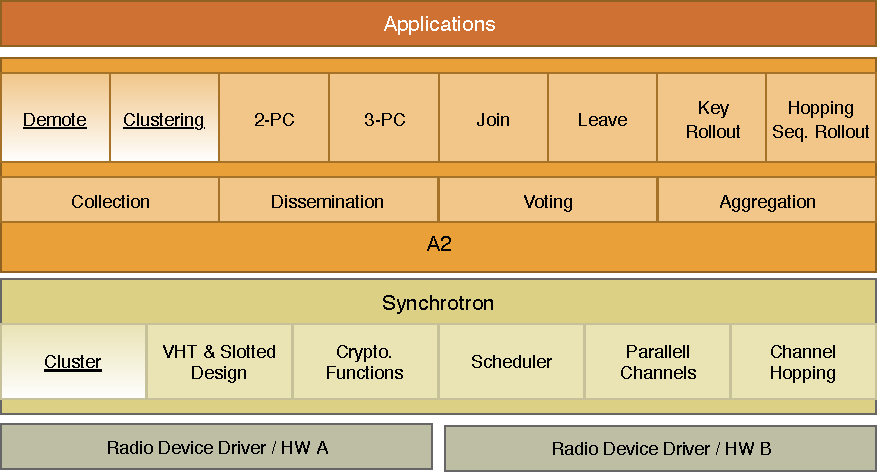
\includegraphics[width=0.7\textwidth]{figure/architecture.pdf}
    \caption{\textbf{Layered system architecture of \atwo{} \cite{a2-introduction-paper}.} Shows the placement of the cluster and demote modules in relation to the other modules. The Cluster module is required in Synchrotron to handle per-cluster channel hopping, association and scheduling modifications. The Clustering and demote services in \atwo{} contains the logic for electing and demoting cluster heads respectively.}
    \label{fig:a2-architecture}
\end{figure}

\subsection{Association}
%Before a node can communicate using the \atwo{} protocol, it has to associate with another node that is already a part of the network. In the beginning, the initiator starts the communication and acts as the source of truth for information regarding current round number, next application to be scheduled, and timing parameters for the communication among other things. When a node is trying to associate with the network, it listens for transmissions while occasionally hopping between random channels to maximise its chances to get a valid packet.

%Usually, all nodes will associate with the network when they start up, however, if a node does not receive a valid packet for some rounds or experiences a failure it will reassociate. The time, until all nodes have associated with the network (in rounds), is $\mathcal{O}(d)$, where $d$ is the diameter of the network. The reason for this time complexity is because a node shuts itself down until the next round as soon as it associates with the network.

With clustering implemented on \atwo{} we have to handle the fact that the network could already be partitioned into clusters when a node tries to associate with the network. If a node receives a packet from another node that is already in a cluster, and we are not currently in the process of clustering the network, the node joins that cluster. 

\subsection{Separating the Cluster Communication}
\label{subsec:separating-the-clusters}
We separate the clusters in two different ways. First, we use a modified version of the channel hopping in \atwo{}. The original \atwo{} implementation hops between radio channels in two different ways as outlined in \cref{subsec-frequency-agility}. Both a network wide predetermined sequence which all nodes follow to different channels and by using parallel channels, randomly selected from a small set. In our implementation, we separate the clusters into different channels. We deactivate the parallel channels functionality since one cluster should not be large enough to generate interference for itself. The nodes still follow the original hopping sequence but offset the channel number by the \textit{cluster-index}. The cluster-index is unique, deterministic and since it is an index the numbers are sequential which makes it ideal to use for this purpose.

Second, each node includes its cluster id in the packet header; if a node receives a packet from another cluster, the node discards that packet. During CH rounds they do not check this condition since all nodes are acting as forwarders. Moreover, during CH rounds, the constructive interference used by \atwo{} in the completion phase does not work. It does not work because CHs include their cluster id in all packets they send, which means that the packets in the completion phase are not equal. A possible solution could be to set the cluster id to 0 during CH rounds. Cluster ids are not used in the inter-cluster communication. However, if a node tries to associate with a packet containing no cluster id, it will not be able to join a cluster and therefore go back to associating. Due to time constraints we have not explored any other possible solutions for this problem.

\subsection{Forwarders During Cluster Head Rounds}
Since the HEED algorithm aims to assign non-overlapping cluster-heads, the communication between the cluster heads requires assistance to function. Therefore, during CH-rounds all non-CH nodes act as forwarders. We implement the forwarders by letting all nodes run the max application as usual but with the modification that nodes suggest 0 as their maximum value which is always overwritten by the CHs actual max value.

A more general implementation is possible since forwarders do not propose any new information by themselves they only require the knowledge of how to merge two packets for an application. We did, however, not implement such a solution since the \atwo{} model does not let the applications provide an operator for combining two payloads. If applications would provide that merge operation through an interface, then a more general implementation in \atwo{} could use the current running applications knowledge of how to merge packets without actually running the application. 


\subsection{flags field for Cluster Heads}
To separate CH rounds from cluster rounds, the nodes switch back and forth between intra- and inter-cluster communication every other round. However, during the join service, no CH rounds are executed. The reason for this is that while the join service's purpose is to build the flags field used for completion during communication within the clusters, the CH has their join process during the cluster service. Therefore, the CH already knows how they perform completion when the join service starts. More specifically, during the clustering service, the CHs builds a list of all CHs. Each CH then uses the index of their entry in this list as their index in the flags field. This both ensures that the CHs has sequential indexing of the flags field, and also know the length of the flags field. During CH rounds the CHs still use the same procedure as during cluster rounds; however, their index in the flags field corresponds to their index in the CH list built during the clustering service.

\subsection{The Initiator}
\label{subsec:implementation_the-initiator}
In our implementation, there are three different phases of the protocol, and the initiator is different in each of them. First, when either the clustering service or the demote service is running, the network is using a single preconfigured node as the initiator. Second, during cluster rounds each CH acts as the initiator in their cluster; since each cluster communicates on separate channels and every initiator runs synchronously with the other CHs, this does not create any conflicts in the network. Third, during CH rounds, to avoid having more than one initiator in the network the first CH in the CH list initiates the network communication.

Switching the initiator between different nodes introduce problems which we did not foresee. Namely, the network can end up in a state where no node consider themselves initiator and the network spends the rest of the time associating. What happens is one of two cases. Either, the preconfigured initiator node loses connection with the network during a round where it does not consider itself initiator and does not regain the connection before the network collectively switches to use that node as initiator again. Alternatively, the CH that is initiator during CH rounds loses connection to the network and demotes itself, the network cannot handle this case, and there will be no initiator during CH rounds until the network executes the clustering service again. 

We can mitigate both of these cases using a number of solutions. We briefly discuss two of them here together with their strengths and weaknesses. First, always using the preconfigured initiator regardless of the state of the network would completely solve this problem. However, this would create an even higher dependency on this node, increasing its energy usage potentially reducing the lifetime of that node and therefore the network. Furthermore, we would have to handle the cluster the preconfigured node joins as a special case to avoid having two initiators in that cluster. Second, we could use a fallback error handling scheme. If the preconfigured initiator is stuck associating it could assign itself as initiator again due to one of two triggers. First, it could use a timeout of some number of rounds; if it does not receive any packet before the timeout triggers, it assumes that the whole network is stuck associating and needs someone to be the initiator. Second, if its estimated time reaches a round in which it should be the initiator, for instance, when the clustering service should be running, it just starts broadcasting as the initiator, assuming the rest of the network will follow. This solution is, however, not very reliable. It assumes that the initiator node can keep correct time synchronisation without any external input, if its clock drifts too much it could wake up at the wrong time and start transmitting erroneous packets to the network. Nevertheless, this could prevent an unrecoverable standstill of the network.



\subsection{Interaction Between Services}
\label{subsec:interaction-between-services}
In this thesis, we implement two different services, the clustering service and the demote service. Furthermore, we use the join service provided by the \atwo{} protocol within the clusters to get consistency in the membership. However, for these applications to work properly, they have to be run in a specific order. First, the clustering service needs to be run and converge on a set of valid CHs. Following that, the network executes the join service within each cluster. Then the demote service is executed, by running the join service before the demote service each CH know how many nodes joined their cluster and can, therefore, make the decision to demote themselves or not. When the demote service is done, the join service needs to be rerun, since the clusters might have changed the network needs to make sure that any node that changed cluster is correctly picked up by that cluster. At this point the clustering process is complete, and operation of the network can resume as normal.




\section{The Clustering Service}
In this section, we explain some implementation specific details that are related to the clustering service. We go into detail about the packet payload, what information we transmit from a node and why; we also talk about issues we face due to not having completion flags. Finally, we talk about the catch-up mechanism we implemented in the clustering service to handle nodes joining the clustering process late.

\subsection{The Cluster Service Packet Payload}
As mentioned in the design chapter, the clustering service exchanges much information to inform the network of how many cluster heads have announced themselves. In this section, we describe the packet's content, why we include that information in the payload and the limitations we encountered when using this structure in the payload.

The cluster service payload contains information both about the cluster heads the transmitting node knows about and information about that node. The content of the cluster service packet payload is summarised in \cref{table:cluster-service-packet}. The cluster head list contains all the cluster heads the transmitting node knows about. The list contains information about the ID; the hop count; and the status of each cluster head, which is either \emph{Tentative} or \emph{Final}. The cluster head list uses three bytes of space per entry in the list with a maximum of 90 bytes allowing 30 entries. The transmitting node also includes its ID in the packet; this information is used in the clustering service to approximate the distance to other nodes as well as how dense the network is. The last entry is consecutive cluster rounds which is a counter that contains information about how many rounds has elapsed since the clustering service started to run; we use this parameter in the catch-up mechanism which we explain in \cref{subsec:catch-up-mechanism}. 

The packet payload size is restricted by the maximum packet size for the IEEE 802.15.4 standard, which is 127 bytes \cite{IEEE-802-15-4}. It is restricted further by the \atwo{} header size and some link layer data, giving us a maximum of 112 bytes for the payload size. As can be seen in \cref{table:cluster-service-packet}. We leave 22 bytes of space in the packet for two reasons. First, some features which we are not using in \atwo{} take up space in the packet header, we do not want the clustering service to break when other unrelated features are used. Second, by leaving some space, we allow more information to be added at a later date if someone should so decide.

\subsection{Clustering Without Completion Flags}
There are two problems introduced by the fact that we cannot run the consistent group membership protocol (the join service) before the clustering service. The problems are both caused by the restriction of the packet size. These two problems impose a hard limit on the number of CHs that can announce themselves in the network as well as increase the amount network of communication that occurs in the clustering service.

The first problem is that the clustering service does not have any flags field it can use to keep track of which nodes have learnt of which clusters. Using such a field would impose a limit on the total number of nodes the protocol can handle, and it would directly contradict one of the primary goals of this thesis, namely scaling. However, without the flags field, we cannot perform completion flooding or early turnoff, two prominent features of the Chaos protocol \cite{chaos-introduction-paper}. However, it is vital that all nodes learn of all CHs since they use this list as a substitute for the join service when running CH rounds. To increase the likelihood of the cluster head list being consistent across all nodes we store the packet payload in two different variables, one that represents the current knowledge of the network and one that represents this specific nodes knowledge. The first variable is reset at the beginning of every round forcing all CHs to transmit their status as CH again while the second variable is stored between rounds so that a node cannot forget anything it has learned so far.  By forcing the network to agree on a set of CH every round we increase the amount of network communication and thus the chance that any particular node will learn of the CHs that have announced themselves.

The size of the CH list in the packet payload causes the second problem. Since we use the list to substitute indices assigned by the join service, it has to be consistent across all nodes, which means that we can never have more CHs in the network than the maximum size of this list. It is not possible to discard CHs that, for example, are outside of a nodes competition radius since then some parts of the network would not consider that CH when calculating their completeness.

These two problems are a limitation on our implementation. It should be entirely possible to modify the consistent group membership protocol so that it can not only run for each cluster but also for the cluster heads eliminating the need for the clustering service to be consistent in that regard. Nodes could then filter out the CHs that are outside of their competition radius since no nodes should join a CH outside that parameter value. However, due to time limitations, we have not explored this implementation any further.




\begin{table}[bt]
\centering
\caption{The parameters and their sizes in the cluster service packet payload.}
\label{table:cluster-service-packet}
\begin{tabular}{|l|l|}
\hline
\textbf{Name}               & \textbf{Size(bytes)} \\ \hline
Cluster head count          & $1$                    \\
Source ID                   & $1$                    \\
Received packets count      & $24$                    \\
Cluster head list           & $3*30=90$              \\
Consecutive cluster rounds  & $1$                    \\ \hline
\textbf{Total}              & \textbf{95}          \\ \hline
\end{tabular}
\end{table}

\subsection{The Catch-up Mechanism}
\label{subsec:catch-up-mechanism}
By the definition of the HEED protocol, every node doubles the probability to announce themselves as tentative cluster heads each round. However, there is a problem if a node associates with the network during the execution of the clustering service. Specifically, its probability to announce itself as CH, $CH_{prob}$, will have fallen behind compared to other nodes; this is most noticeable in the early rounds of the network during the initial association of all nodes. For example, nodes associating with the initiator in round one randomises their initial $CH_{prob}$ in round two. However, in round two the initiator has already doubled its own $CH_{prob}$. As a remedy, we implemented a \textit{catch-up mechanism}. In the cluster service's packet payload, we attach a counter for the number of consecutive cluster rounds which a node saves once received. At the beginning of later rounds, they increment the counter before transmitting it on. The counter describes the number of times each node's initial $CH_{prob}$ should have doubled since the start of the clustering service. An advantage remains for nodes already part of the network or the ones which join earlier in the service, since they have had more chances to announce themselves as CH. However, as \cref{tab:prob-no-catchup} and \cref{tab:prob-catchup} show this advantage is very small.

\begin{table}[bt]
\centering
\caption{Probability that a node has announced itself as CH at a specific round without the catch-up mechanism.}
\label{tab:prob-no-catchup}
\begin{tabular}{|c|c|c|cccccc|}
\hline
\textbf{Round(r)} & \textbf{$CH_{Prob}$} & \multicolumn{7}{c|}{\textbf{Cumulative probability starting at round r}}                                                                                       \\ \hline
1                 & 0.005                & 0.005 &                            &                            &                            &                            &                            &       \\ \cline{1-4}
2                 & 0.010                & 0.015 & \multicolumn{1}{c|}{0.005} &                            &                            &                            &                            &       \\ \cline{1-5}
3                 & 0.020                & 0.035 & \multicolumn{1}{c|}{0.015} & \multicolumn{1}{c|}{0.005} &                            &                            &                            &       \\ \cline{1-6}
4                 & 0.040                & 0.073 & \multicolumn{1}{c|}{0.035} & \multicolumn{1}{c|}{0.015} & \multicolumn{1}{c|}{0.005} &                            &                            &       \\ \cline{1-7}
5                 & 0.080                & 0.147 & \multicolumn{1}{c|}{0.73}  & \multicolumn{1}{c|}{0.035} & \multicolumn{1}{c|}{0.015} & \multicolumn{1}{c|}{0.005} &                            &       \\ \cline{1-8}
6                 & 0.160                & 0.284 & \multicolumn{1}{c|}{0.147} & \multicolumn{1}{c|}{0.073} & \multicolumn{1}{c|}{0.035} & \multicolumn{1}{c|}{0.015} & \multicolumn{1}{c|}{0.005} &       \\ \hline
\textbf{7}                 & \textbf{0.320}                & \textbf{0.513} & \multicolumn{1}{c|}{\textbf{0.284}} & \multicolumn{1}{c|}{\textbf{0.147}} & \multicolumn{1}{c|}{\textbf{0.073}} & \multicolumn{1}{c|}{\textbf{0.035}} & \multicolumn{1}{c|}{\textbf{0.015}} & \textbf{0.005} \\ \hline
\end{tabular}
\end{table}

    
\begin{table}[bt]
\centering
\caption{Probability that a node has announced itself as CH at a specific round with the catch-up mechanism.}
\label{tab:prob-catchup}
\begin{tabular}{|c|c|c|cccccc|}
\hline
\textbf{Round(r)} & \textbf{$CH_{Prob}$} & \multicolumn{7}{c|}{\textbf{Cumulative probability starting at round r}}                                                                                       \\ \hline
1                 & 0.005                & 0.005 &                            &                            &                            &                            &                            &       \\ \cline{1-4}
2                 & 0.010                & 0.015 & \multicolumn{1}{c|}{0.010} &                            &                            &                            &                            &       \\ \cline{1-5}
3                 & 0.020                & 0.035 & \multicolumn{1}{c|}{0.030} & \multicolumn{1}{c|}{0.020} &                            &                            &                            &       \\ \cline{1-6}
4                 & 0.040                & 0.073 & \multicolumn{1}{c|}{0.069} & \multicolumn{1}{c|}{0.060} & \multicolumn{1}{c|}{0.040} &                            &                            &       \\ \cline{1-7}
5                 & 0.080                & 0.147 & \multicolumn{1}{c|}{0.143} & \multicolumn{1}{c|}{0.134} & \multicolumn{1}{c|}{0.117} & \multicolumn{1}{c|}{0.080} &                            &       \\ \cline{1-8}
6                 & 0.160                & 0.284 & \multicolumn{1}{c|}{0.280} & \multicolumn{1}{c|}{0.273} & \multicolumn{1}{c|}{0.258} & \multicolumn{1}{c|}{0.227} & \multicolumn{1}{c|}{0.160} &       \\ \hline
\textbf{7}                 & \textbf{0.320}                & \textbf{0.513} & \multicolumn{1}{c|}{\textbf{0.511}} & \multicolumn{1}{c|}{\textbf{0.506}} & \multicolumn{1}{c|}{\textbf{0.496}} & \multicolumn{1}{c|}{\textbf{0.474}} & \multicolumn{1}{c|}{\textbf{0.429}} & \textbf{0.320} \\ \hline
\end{tabular}
\end{table}


To motivate the advantage of having the catch-up mechanism we present the probability that a node has announced itself as CH after round $r$ without the catch-up mechanism in \cref{tab:prob-no-catchup} and with the catch-up mechanism in \cref{tab:prob-catchup}. The current starting probability of a node with maximum energy in our implementation is $CH_{prob} = 0.005$. Since the probability for a node to announce itself as CH is independent in each round, we can calculate the probability of a node having announced itself in the first $r$ rounds using the formula:

\begin{equation}
1 - \prod_0^r (1 - 2^rCH_{Prob}).   
\end{equation}

Looking at \cref{tab:prob-no-catchup} and \cref{tab:prob-catchup} the most interesting data points are the two bottom rows, emphasised in bold. Without the catch-up mechanism, there is a significant difference in the cumulative probability that a node has announced itself as CH. However, with the catch-up mechanism, the difference is minimal except for in the most extreme case when a node starts at round seven, compared to a node that started at round one. A specific example shows that when we do not use the catch-up mechanism a node that starts the clustering service at round three will at round seven have a $0.513 - 0.147 \approx 38$ percentage points less chance of having announced themselves as CH compared to a node that started at round one. However, with the catch-up mechanism the difference is only $0.513 - 0.506 \approx 0.7$ percentage points. The same pattern can be seen for other starting points as well, giving a clear motivation that the catch-up mechanism is useful. 

Another solution, which on the surface would seem to be fairer, would be to calculate the cumulative probability that a node should have announced itself if they would have been present from the beginning. Try to announce itself once using that probability, and then continue with the usual probabilities. However, consider a node which starts the clustering service together with the initiator, fails a couple of rounds later and then associates with the initiator again continuing with the clustering service. If we implement this solution, then a node that performed this sequence of events would have an advantage compared to nodes that did not fail. The advantage could be taken into consideration and excluded, but we chose the catch-up mechanism for its simplicity compared to the solution just described.





\subsection{The Demote Service}
The demote service is responsible for removing CHs that are considered suboptimal. It demotes all CHs which have fewer nodes in their cluster than the parameter \emph{minimum cluster size}. As we mention in \cref{subsec:interaction-between-services}, the join service is required to run before and after the demote service to ensure both that the demote service knows which CHs to demote and also for the user application to behave correctly.

The demote service behaves similarly to the clustering service; each CH decides to demote itself locally. The service is then run for some number of rounds to ensure that the information spreads to the whole network. At the end of the last demote service round each demoted CH, and all nodes that joined them select a new CH from the list of CHs that remain. Additionally, all nodes update their cluster indices according to the new list after they have removed all demoted CHs from the CH list.


% RESULTS
\chapter{Evaluation}
\label{chap:evaluation}
In this chapter, we evaluate our clustering implementation. We begin by defining the topologies and the metrics we use. We continue with an evaluation of our clustering parameters, where we determine what configurations of the parameters yield the most reliable and stable network, for different topologies. Next, we compare our clustering implementation to the \atwo{} system. We end this chapter with a discussion on the evaluation results, how our limitation on fault tolerance affected our results, and running different applications in a clustered network.


\section{Evaluation Setup}
We run several different tests to evaluate our clustering implementation. In this section, we describe our test setup, the network topologies we run our tests on, and the metrics we use. 

\subsection{The Cooja Simulator}
\label{subsec:cooja-setup}
Cooja \cite{Osterlind2006-cooja-introduction} is a simulator for ContikiOS \cite{Dunkels2004-contiki-introduction}, the operating system that Chaos and \atwo{} are implemented on \cite{chaos-introduction-paper, a2-introduction-paper}. In Cooja, we create networks with 50 and 200 nodes placed randomly in topologies of different sizes, to get both dense and sparse networks. We start with 50 nodes in a 100x100 $m^2$ area and increase the side of the square in steps of 300 meters up to 2500x2500 $m^2$. We do the same for 200 nodes but only up to 1300x1300 $m^2$. We only have one network topology per area and number of nodes. We simulate each test for 30 minutes, which gives us 600 rounds of data. 

We run most of our tests using 50 nodes for two reasons. First, 50 nodes are enough to see that the Clustering service creates several clusters. Second, running these simulations takes a significant amount of time, and it does not scale well when increasing the number of nodes. Simulating 30 minutes with 50 nodes takes 2-3 hours, and 200 nodes takes 30-50 hours on our hardware. However, when comparing our clustering process to the \atwo{} system, we also simulate 200 nodes to see the effects of scaling up the network. Moreover, we chose the different sizes from the fact that in Cooja, a network with an area of 100x100 $m^2$ ensures that is is a 1-hop network and at 2500x2500 $m^2$ the network is at least a 7-hop network.

\subsection{The Flocklab Testbed}
The Flocklab testbed \cite{Lim2013-flocklab-introduction} consists of 27 nodes deployed both indoors and outdoors at ETH Zurich. Flocklab provides several services that make it easy to measure and evaluate the code that is running on the nodes. Our tests log data to the serial port of an observer node, Flocklab aggregates the data and sends it to us at the end of each test. 


\subsection{Metrics}
\begin{newtext}
To define the metrics we use, we make a distinction between rounds which execute coordination and rounds which execute applications. Coordination is rounds in which the network is set up to enable applications to run; coordination includes the Cluster, Join, and Demote services. We also differentiate between static and dynamic coordination. Static coordination is scheduled at fixed round intervals to, for example, cluster the network. Dynamic coordination, on the other hand, is scheduled by nodes as needed during the application phase, to handle faults in the network or new nodes. Applications are programs that run with the goal of providing some value or perform some calculation; Some examples of applications are finding the maximum or mean of all values proposed by nodes in the network, or performing a two-phase commit.

We consider four metrics when evaluating clustering on \atwo{}: stability, reliability, latency, and energy usage. We define the metrics for one execution of a network, that is, one simulation in Cooja or one run on the Flocklab testbed.


\paragraph*{Stability} is a measurement of how often topology changes occur. We say that a node is stable if it is executing an application and unstable if it is executing dynamic coordination. Stability during one round is the proportion of nodes that are stable. We give the following definition for the stability for one test. 


\begin{Definitions}{}{}
Let $s_i$ be the set of stable nodes in round $i$, $n$ the set of all nodes, and $R$ the set of all rounds which do not execute static coordination.

\begin{equation*}
    Stability = \frac{\sum\limits_{i \in R}{|s_i|}}{|n|*|R|}
\end{equation*}

\end{Definitions}

\paragraph*{Reliability} is a measurement of how well an application runs on the network; thus, it is only measured during application rounds. Reliability during one round is the proportion of stable nodes that successfully execute an application. We give the following definition for the reliability for one test.

\begin{Definitions}{}{}
Let $a_i$, $a_i \subset s_i$, be the set of stable nodes that succeeds with an application in round $i$, and $R_a$ the set of all rounds in which an application is executed.


\begin{equation*}
    Reliability = \frac{\sum\limits_{i \in R_a}{|a_i|}}{\sum\limits_{i \in R_a}{|s_i|}}
\end{equation*}

\end{Definitions}


\paragraph*{Latency} is a measurement of how long it takes for an application to terminate. For a stable node in one round, latency is the number of slots from the start of the round until the node powers down. We give the following definition for the latency for one test.

\begin{Definitions}{}{}
Let $l_{ij}$ be the latency for node $j$ in round $i$.

\begin{equation*}
    Latency = \frac{\sum\limits_{i \in R_a}{ \sum\limits_{j \in s_i}{l_{ij} } }}{\sum\limits_{i \in R_a}|s_i|}
\end{equation*}
\end{Definitions}


\paragraph*{Energy usage} is a measurement of the average amount of energy used by a node per Energest time unit. Energest is the built-in energy estimation module in Contiki and we measure energy usage in all rounds, both during coordination and applications. We give the following definition for the energy usage for one test.


\begin{Definitions}{}{}
Let $e_{i}$ be the energy used by node $i$ in one test, and let $T$ be the running time of the test in Energest time units.

\begin{equation*}
    Energy\ usage = \frac{\sum\limits_{i \in n}{e_{i}}}{T*n}
\end{equation*}
\end{Definitions}

\end{newtext}

\subsection{Limitations}
We impose several limitations on the evaluation of our clustering implementation. We only run tests in the Cooja simulator and on the Flocklab testbed. Running simulations gives us the freedom to choose topologies, but the simulations do not model the network perfectly. Flocklab, on the other hand, contains real nodes but is relatively small with only 27 nodes in a static configuration. We only compare our implementation to \atwo{}, and do not consider any other WSN protocols.

Furthermore, we only simulate two different network sizes, 50 nodes and 200 nodes. We only simulate 50 nodes when searching for parameter values, and include networks with 200 nodes when we compare our clustering process to \atwo{}.

To limit the scope of our parameter evaluation, we use the values listed in \cref{tab:parameter-default-values} for the parameters that we are not currently evaluating.

\begin{table}[bt]
\centering
\caption{The parameters we evaluate and their default values}
\label{tab:parameter-default-values}
\begin{tabular}{r|l}
\textbf{Parameter}                 & \textbf{Value} \\ \hline
Competition Radius                 & 1              \\
Minimum cluster size                 & 4              \\
Nodes per cluster ratio            & 10             \\
Round re-synchronisation threshold & 3             
\end{tabular}
\end{table}

Lastly, we only evaluate clustering using the Max application. The Max application is the most straightforward application currently implemented in the \atwo{} system. We discuss how to apply different applications and the implications of doing so in \cref{subsec:discuss-other-apps}.


\section{Clustering Parameters}
\label{sec:clustering-parameters}
In this section, we experimentally search for optimal values to the parameters in our clustering algorithm. The parameters are \emph{round re-synchronisation threshold}, \emph{competition radius}, \emph{minimum cluster size}, and \emph{nodes per cluster ratio}. We run each parameter configuration three or six times and plot the reliability and stability of each test for each network topology.

We only look at the reliability and stability of these tests since the purpose is to find which parameters yield the best results, in terms of running the application. However, we include the latency results in \cref{app:a} for completeness; we note that there are no significant differences in latency for different values of these parameters, and will not comment on these results any further.

We use a different number of topologies depending on which parameter we evaluate. When evaluating competition radius, we test on all network topologies we describe in \cref{subsec:cooja-setup} since this parameter is dependent on the density of the network. However, when we test the parameters minimum cluster size and nodes per cluster ratio, we use topologies from 100x100 $m^2$ to 1300x1300 $m^2$, using competition radius 1. We argue that increasing the competition radius while simultaneously increasing the area of the networks will not give any new results. By excluding the network topologies with a larger area, we could repeat each configuration for these tests a total of six times, instead of three.

\subsection{Round Re-synchronisation Threshold}
\label{subsec-resync-threshold}
The \emph{round re-sync threshold} parameter is not directly related to the clustering process. Rather, it is a setting that controls a fundamental part of the \atwo{} system. Round re-sync threshold is a numeric parameter that determines how many rounds a node will spend receiving no packets before associating with the network again. 

We evaluate three different values of the round re-sync threshold (1, 2, and 3), for each value of re-sync threshold we evaluate three different values of competition radius (1, 2, and 3), which gives us a total of 9 test configurations. We use different values of competition radius for these tests because we do not want a suboptimal competition radius to affect the results regarding the re-sync threshold, especially for sparser networks.

\begin{newtext}
We make two observations from the round re-sync threshold results, shown in \cref{fig:resync-treshold-tests}. First, the reliability is drastically increased when the re-sync threshold is greater than 1. Second, the stability increases as the re-sync threshold increases. 

The reason reliability is low when the re-sync threshold is 1 (\cref{subfig:resync-treshold-1}), is that a clustered network is not compatible with such a low threshold. The cause of this problem is that the network has a single initiator during CH rounds, which is the CH with the lowest ID. Furthermore, we allow clusters to schedule and run the Join service during CH rounds, meaning those clusters will not participate with their value, neither will they forward packets during CH rounds. 

The problem, which often occurs, is that the cluster with the lowest ID runs the Join service during a CH round, in that case, there is no initiator present for the CH round. Without an initiator, all other clusters that participate in the CH round, will increase their resynchronisation counter by one, reach the resynchronisation threshold, and start associating. Furthermore, as we discuss in \cref{section:evaluation-discussion}, our limitation regarding fault tolerance further exacerbates this problem.

Usually, these scenarios only affect the stability of the network. However, in this case, the reliability is also affected since the network never has a chance to continue normal execution. Since the re-sync threshold is set too low, there is a high probability that every round has some portion of nodes associating, and some portion of nodes running the max application but failing since the only initiator is running the Join service.

\end{newtext}

\begin{newtext}
Furthermore, the stability increases with the re-sync threshold. The increase in stability when increasing the parameter from 1 to 2 follows from the same reasoning as for the reliability. However, the stability continues to increase when going from 2 to 3 as well. With an increase in the re-sync threshold, there is a lower chance that a node will associate with the network since it has a higher chance of receiving at least one valid packet before it reaches the threshold. Thus we see an increase in stability since in a network with a higher re-sync threshold nodes will wait longer before recognising a bad connection and try to re-associate.
\end{newtext}

From this evaluation, we conclude that out of the values we tested, using a re-sync threshold of 3 gives the best results. Even though \cref{fig:resync-treshold-tests} imply a trend of higher stability with an increasing re-sync threshold. However, we did not test greater values of this parameter due to time constraints, we discuss implications of increasing it more in \cref{discussion:clustering-parameters}. All further evaluation of our clustering implementation uses a re-synchronisation threshold of 3.

\begin{figure}[H]
\centering
\begin{subfigure}{\textwidth}
    \centering
    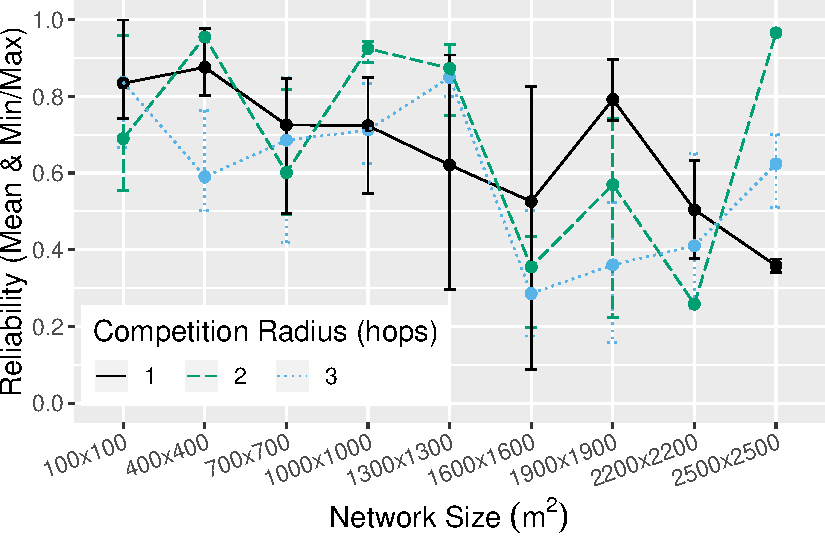
\includegraphics[width=0.49\textwidth, keepaspectratio]{figure/Results/ParameterEvaluation/ResyncThreshold1_Reliability.pdf}
    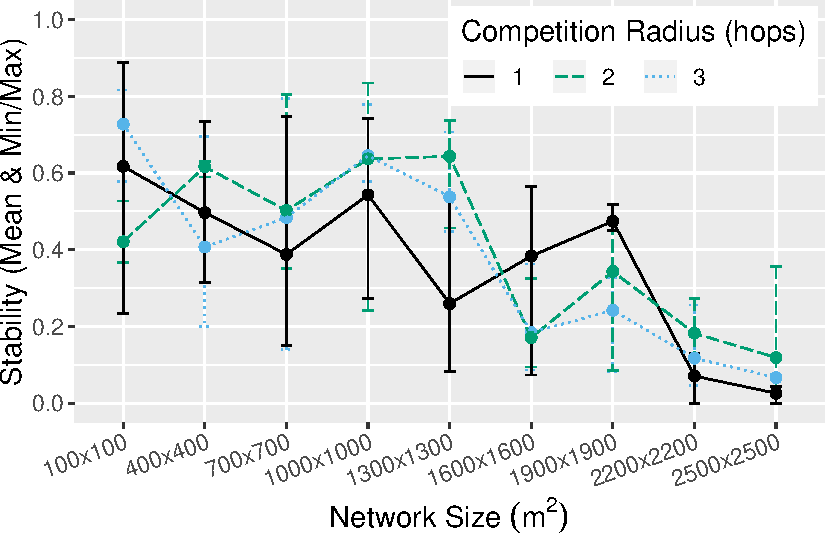
\includegraphics[width=0.49\textwidth, keepaspectratio]{figure/Results/ParameterEvaluation/ResyncThreshold1_Stability.pdf}
    \caption{Re-synchronisation threshold 1.}
    \label{subfig:resync-treshold-1}
\end{subfigure}
\begin{subfigure}{\textwidth}
    \centering
    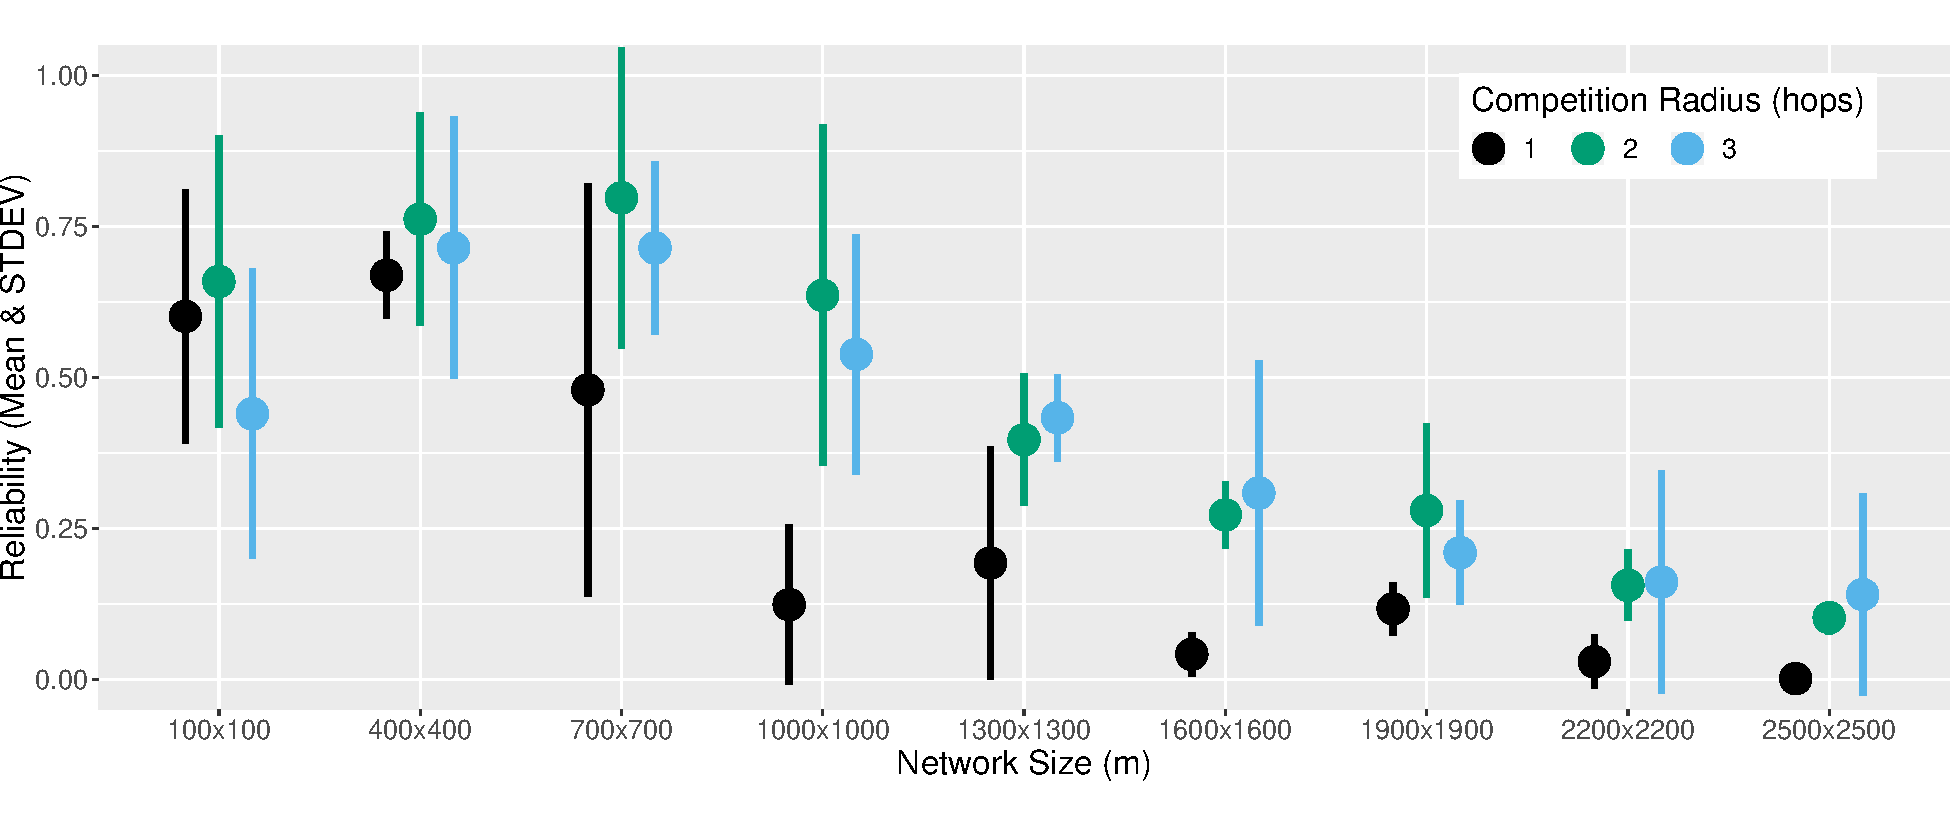
\includegraphics[width=0.49\textwidth, keepaspectratio]{figure/Results/ParameterEvaluation/ResyncThreshold2_Reliability.pdf}
    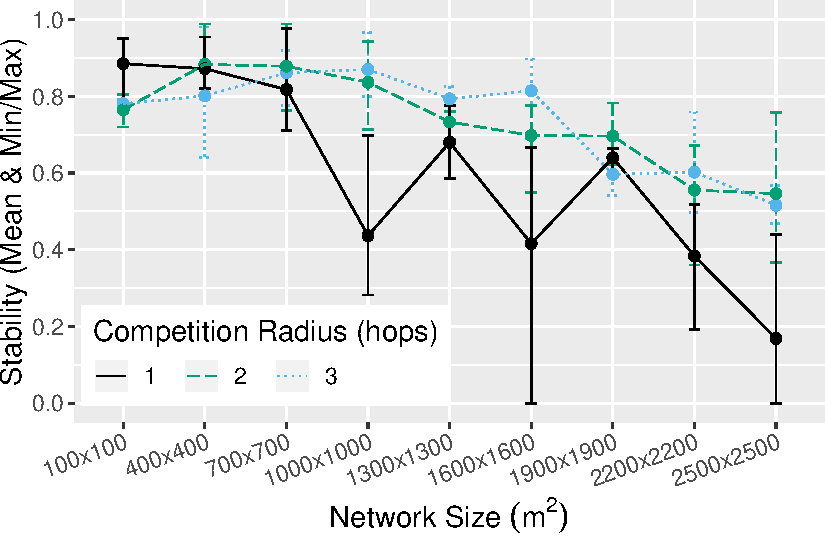
\includegraphics[width=0.49\textwidth, keepaspectratio]{figure/Results/ParameterEvaluation/ResyncThreshold2_Stability.pdf}
    \caption{Re-synchronisation threshold 2.}
    \label{subfig:resync-treshold-2}
\end{subfigure}
\begin{subfigure}{\textwidth}
    \centering
    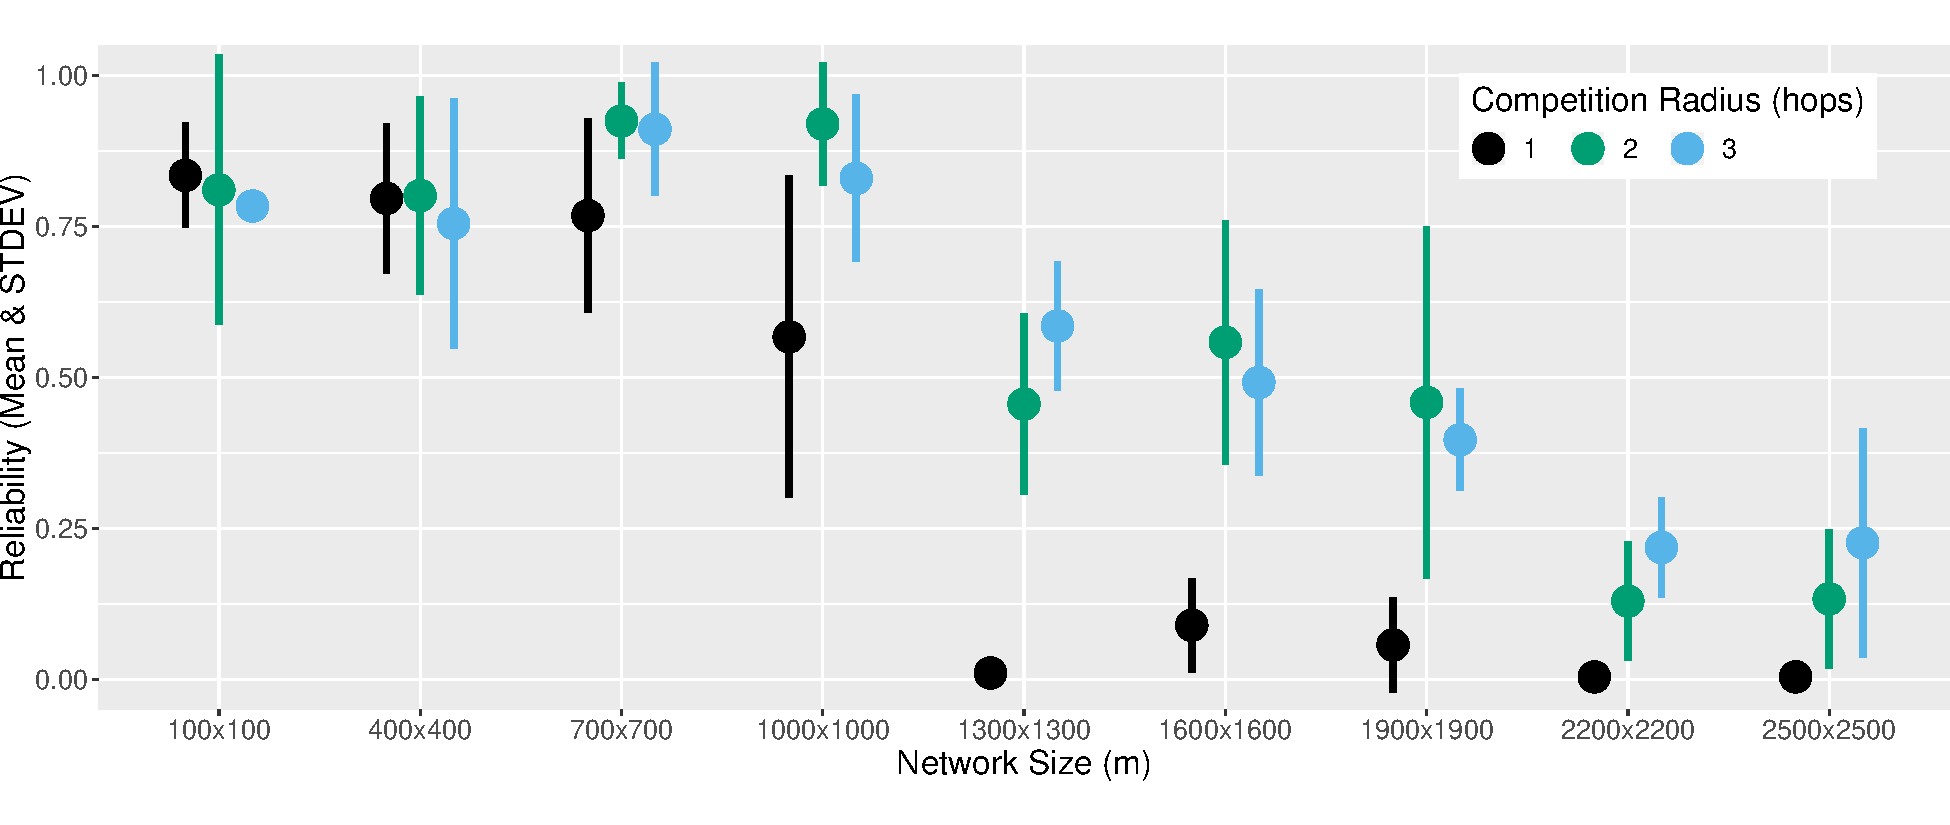
\includegraphics[width=0.49\textwidth, keepaspectratio]{figure/Results/ParameterEvaluation/ResyncThreshold3_Reliability.pdf}
    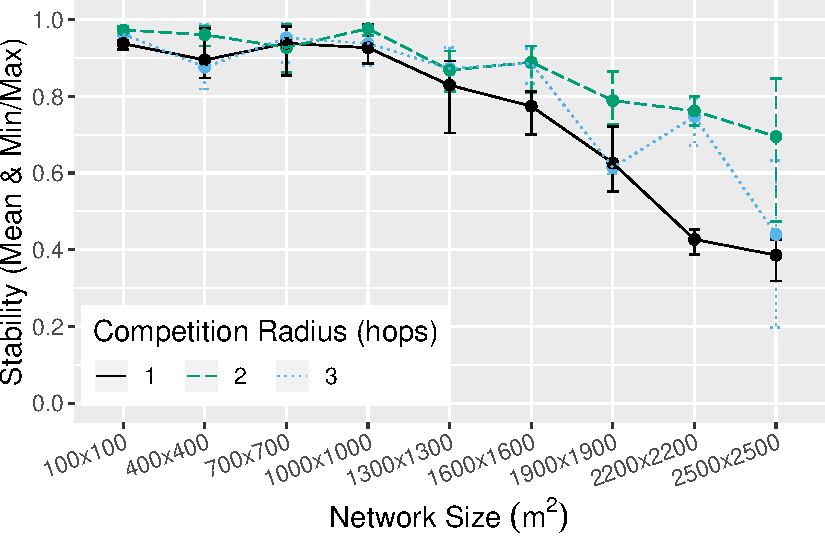
\includegraphics[width=0.49\textwidth, keepaspectratio]{figure/Results/ParameterEvaluation/ResyncThreshold3_Stability.pdf}
    \caption{Re-synchronisation threshold 3.}
    \label{subfig:resync-treshold-3}
\end{subfigure}

    \caption{Resynchronisation threshold tests for different values of Competition radius. Both reliability and stability increases as the re-sync threshold increases.}
    \label{fig:resync-treshold-tests}
\end{figure}


\begin{figure}[bt]
    \centering
    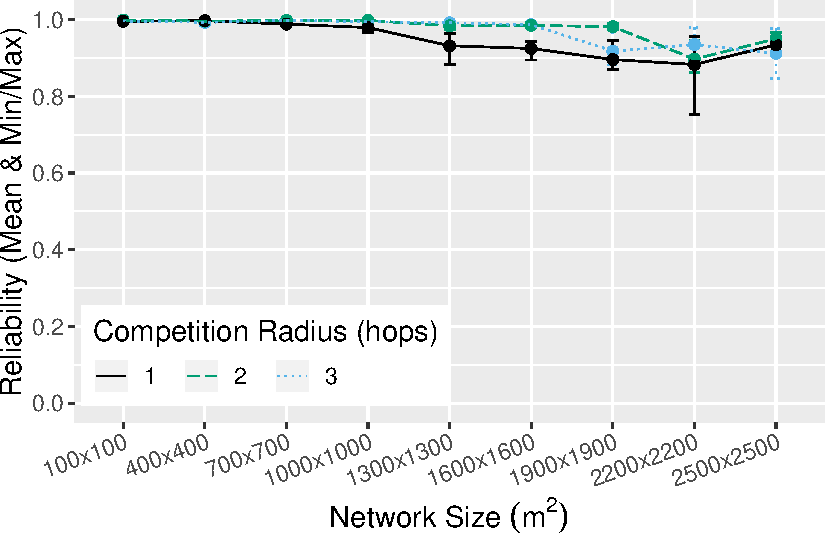
\includegraphics[width=0.49\textwidth, keepaspectratio]{figure/Results/ParameterEvaluation/CompetitionRadius_Reliability.pdf}
    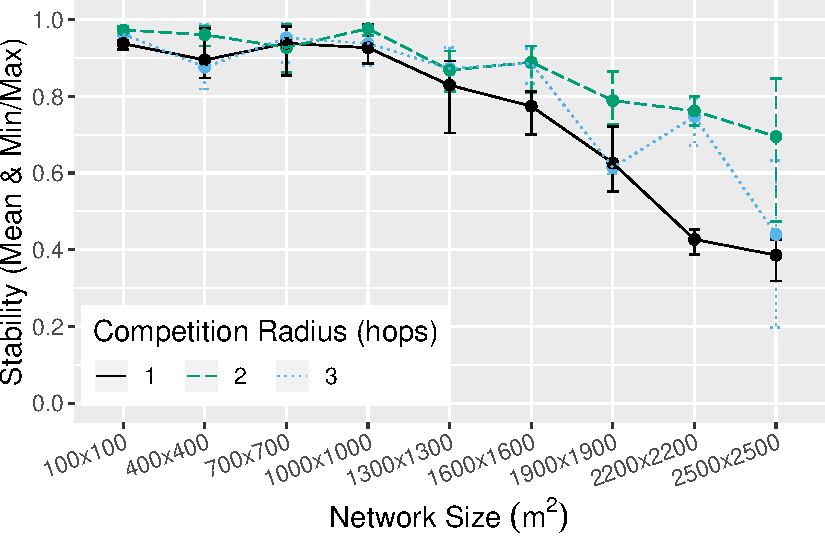
\includegraphics[width=0.49\textwidth, keepaspectratio]{figure/Results/ParameterEvaluation/CompetitionRadius_Stability.pdf}
    \caption{The reliability and stability for different network sizes. Each network size has been tested with competition radius 1, 2, and 3.}
    \label{fig:comp-radius-reliability}
\end{figure}

\subsection{Competition Radius}
\label{subsec:competition-radius}


\begin{newtext}
Competition radius determines the distance, in hops, from which a node can choose a CH. For this parameter, we evaluate the values 1, 2 and 3, which ensures that we test the minimum value of 1 but also not get too sparse clusters. We show the average, minimum, and maximum reliability and stability for each network size and each competition radius in \cref{fig:comp-radius-reliability}. Note that this figure is the same as \cref{subfig:resync-treshold-3} because we set the re-synchronisation threshold to 3 for all tests. Consequently, both of these tests use the same parameter values, so we did not rerun the test.

We see that both reliability and stability decreases as the size of the networks increase. We expect to see this decrease since clustering sparse networks will make them even sparser, which hinders communication. However, we see that higher values of competition radius are better for these networks since larger clusters are created, which does not impact communication as much as small clusters. Furthermore, the differences in stability and reliability for the denser networks (100x100, 400x400, and 700x700) is noise. These networks are 1-hop networks, and thus the competition radius value does not affect the clustering.
\end{newtext}

 
\subsection{Minimum Cluster Size}
Minimum cluster size determines the smallest cluster that is allowed to exist after the clustering process has converged on a set of clusters. All clusters with fewer nodes are removed, and the affected nodes join other clusters. We evaluate this parameter using three different values, 2, 4, and off; off means that no clusters are considered too small. We did not test any larger values for this parameter since we only use 50 nodes for the parameter tests, and a value larger than 4 would mean that more than 10\% of the nodes in the network could be in a cluster and it would be removed, which we consider too aggressive. We show the reliability and stability for these tests in \cref{fig:min-node-count-reliability}.

\begin{newtext}
When we look at the reliability for this parameter, we see that there is no significant difference for any topology or parameter value. However, we see a small variance in stability for larger networks. Looking at the data on how many cluster heads were created and demoted for these tests, which we can see in \cref{fig:minnodecount-chsafterdemotion}, we see two interesting results. First, using higher values of this parameter show no significant difference in the number of CHs created by the clustering process. Second, there was one test which demoted many more CHs than the others, the value 2 for the 100x100 $m^2$ topology. The high number of demoted CHs resulted in the CH count being close to the average. In that test, 32 CHs were demoted while normally 1-2 CHs are demoted. This recovery demonstrates that using this parameter can help the clustering process handle faults in the Clustering service. 
\end{newtext}



\begin{figure}[bt]
    \centering
    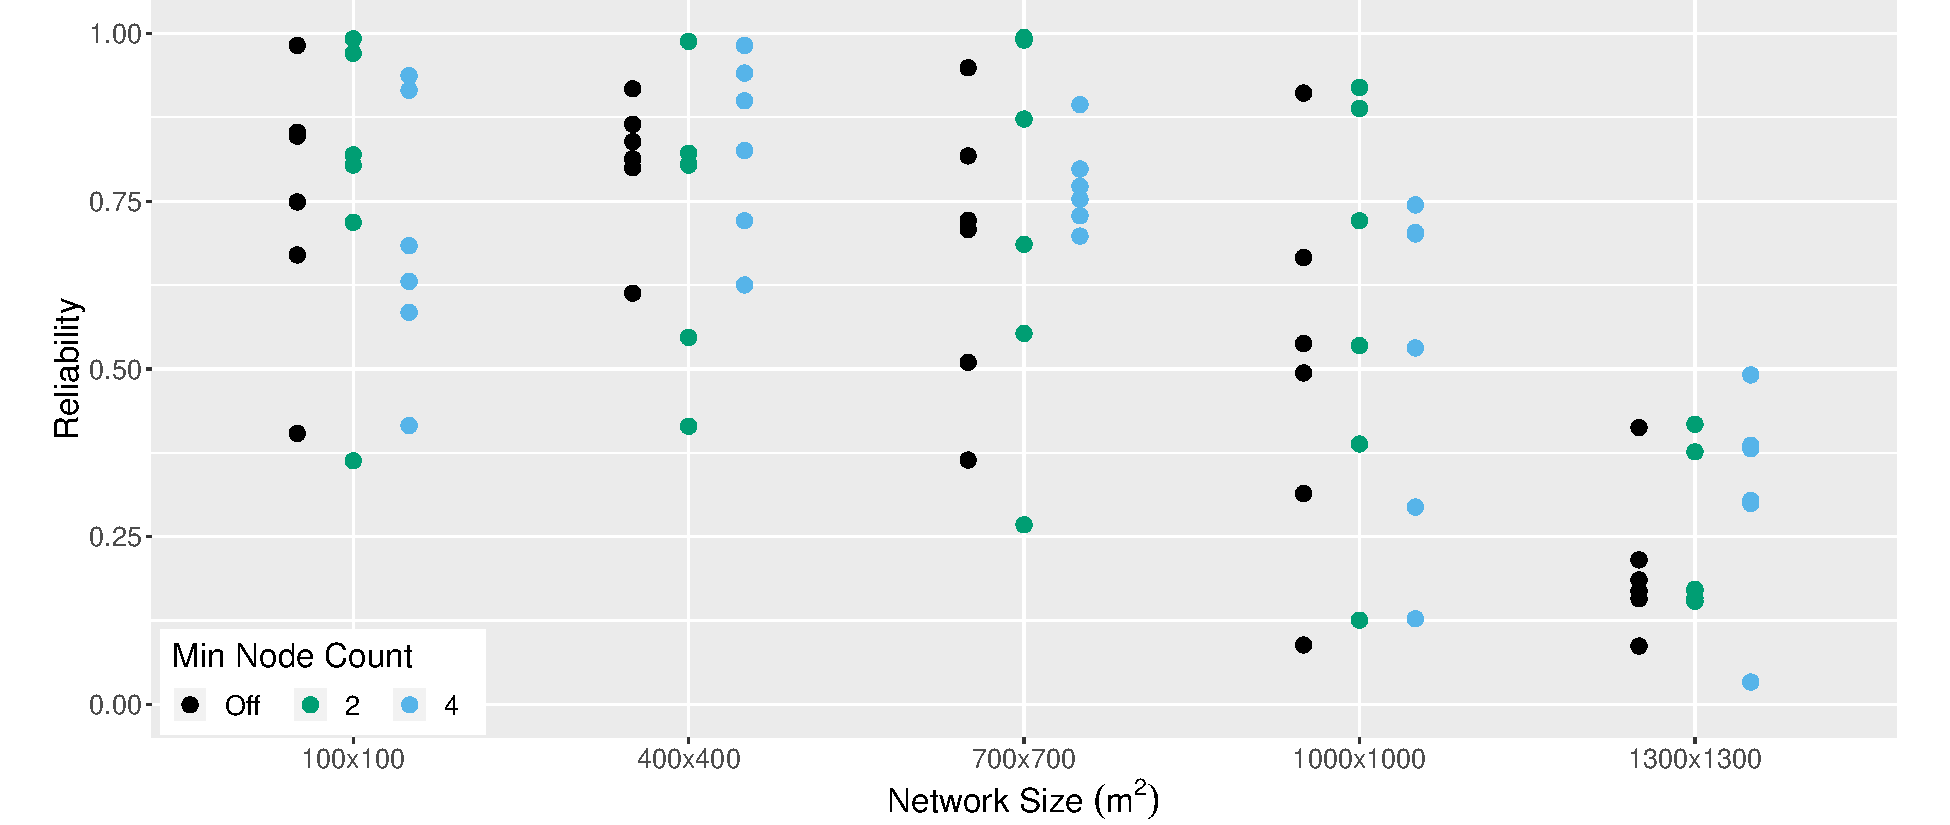
\includegraphics[width=0.49\textwidth, keepaspectratio]{figure/Results/ParameterEvaluation/MinNodeCount_Reliability.pdf}
    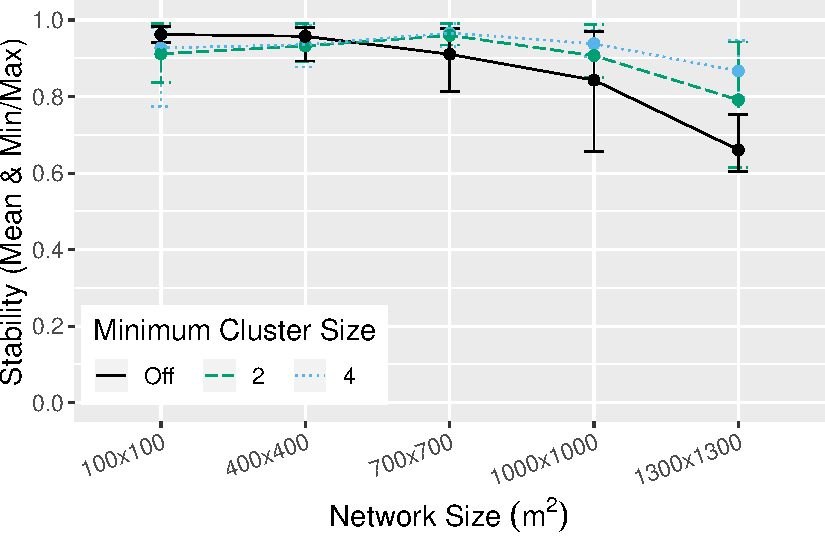
\includegraphics[width=0.49\textwidth, keepaspectratio]{figure/Results/ParameterEvaluation/MinNodeCount_Stability.pdf}
    \caption{The reliability and stability for different network sizes. Each network has been tested with minimum cluster size values off, 2, and 4.}
    \label{fig:min-node-count-reliability}
\end{figure}

\begin{figure}[bt]
    \centering
    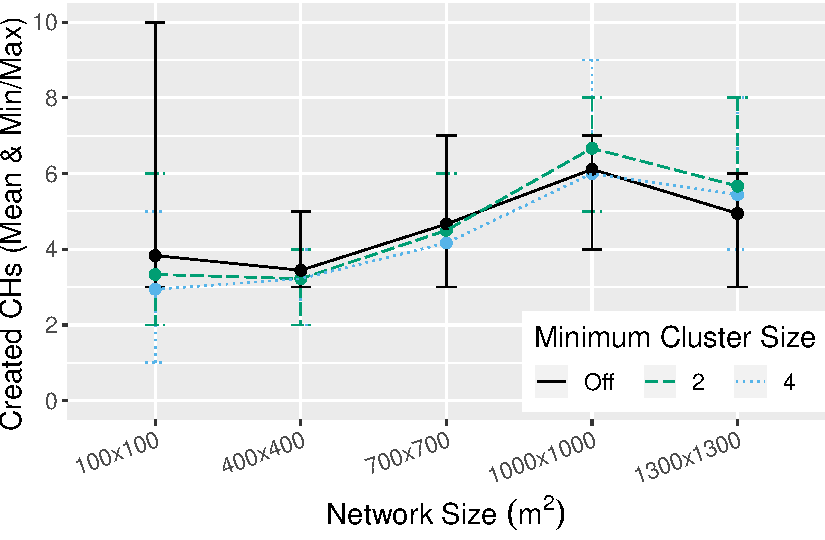
\includegraphics[width=0.49\textwidth, keepaspectratio]{figure/Results/ParameterEvaluation/MinNodeCount_CHsAfterDemotion.pdf}
    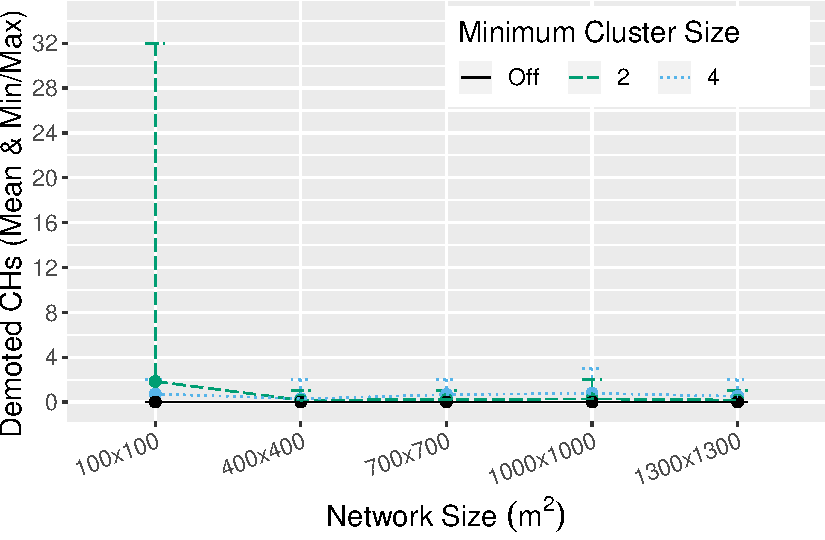
\includegraphics[width=0.49\textwidth, keepaspectratio]{figure/Results/ParameterEvaluation/MinNodeCount_DemotedCHs.pdf}
    \caption{Shows the number of CHs after the clustering process has finished, and the number of demoted CHs.}
    \label{fig:minnodecount-chsafterdemotion}
\end{figure}

\subsection{Nodes per Cluster Ratio}
\label{subsec:nodes-per-cluster-ratio}
The \emph{nodes per cluster ratio} parameter determines if nodes may become CHs even if they have heard from another CH within the competition radius. The parameter describes a ratio of how many neighbours a node needs to have relative to the number of CHs the node has heard. We test the values 5, 10, 15, and off for this parameter. The value off means a CH will never announce itself if it has heard from another CH within the network's competition radius. The results can be seen in \cref{fig:nodes-per-cluster-ratio-reliability}.

\begin{newtext}
The most significant results for the nodes per cluster ratio parameter is the decrease in stability and reliability in the 1000x1000 and 1300x1300 $m^2$ networks. With more clusters in networks with a larger area, we see more clusters failing with communication, causing nodes to try and re-synchronise, which is worsened by our limitation on fault tolerance. Furthermore, the two deviations in stability for 100x100 $m^2$ in the case of 10 and 15 nodes per cluster ratio are both due to noise.

Additionally, we see a small but constant decrease in reliability for the parameter value 5. This decrease is because the Clustering service creates too many clusters which are only demoted or otherwise removed, as can be seen in \cref{fig:nodes-per-cluster-ratio-promoted-ch-count}. Since demoting a CH may cause a fault, increasing the number of demotions will increase the probability of a fault to occur. Usually, these scenarios only affect the stability of the network, but in this case, the reliability is also affected since the CHs could not agree on which CHs was demoted and thus never agree on the correct maximum value in the CH rounds.

Nonetheless, we noticed that more nodes announced themselves as CH with a smaller nodes per cluster ratio value as seen in \cref{fig:nodes-per-cluster-ratio-promoted-ch-count}; this shows that the parameter works as intended but requires careful consideration when configured, and needs to be adapted to the network topology.

\end{newtext}

\begin{figure}[bt]
    \centering
    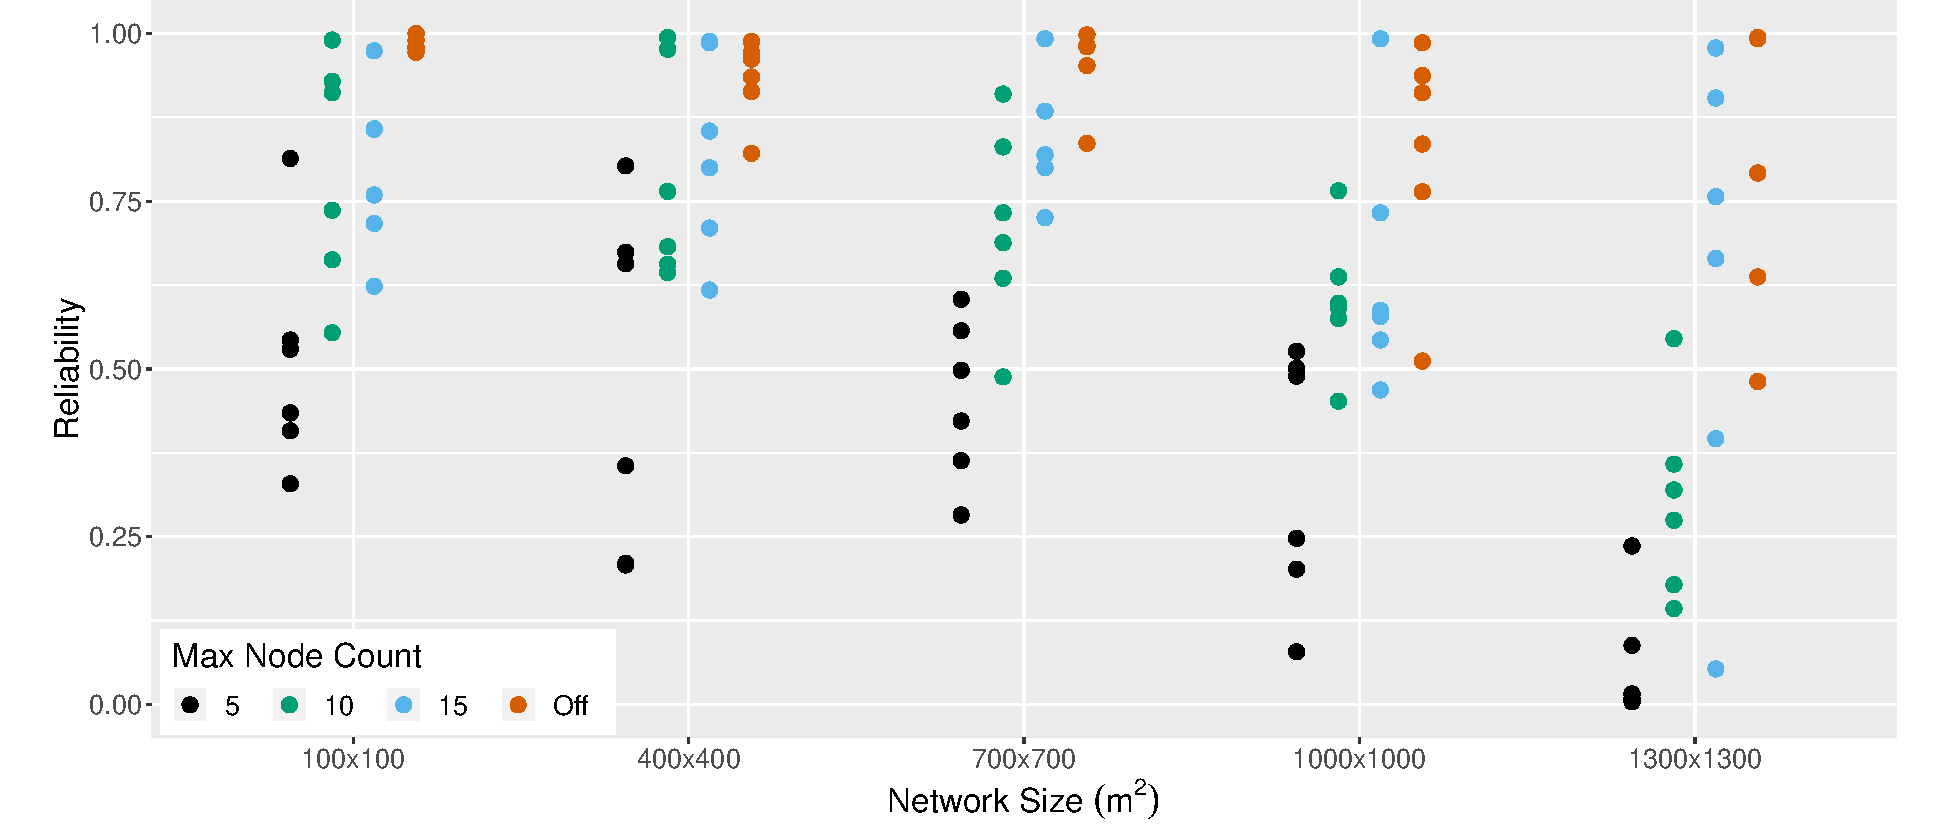
\includegraphics[width=0.49\textwidth, keepaspectratio]{figure/Results/ParameterEvaluation/MaxNodeCount_Reliability.pdf}
    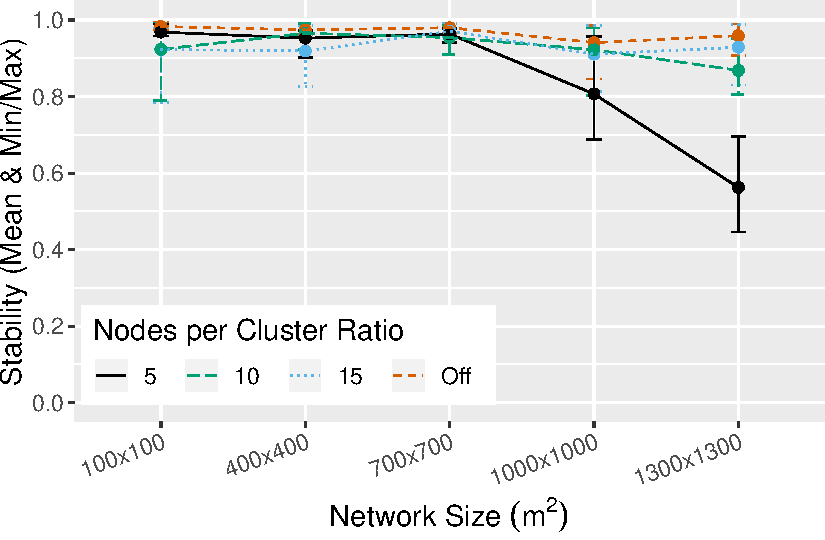
\includegraphics[width=0.49\textwidth, keepaspectratio]{figure/Results/ParameterEvaluation/MaxNodeCount_Stability.pdf}
    \caption{The reliability and stability for different network sizes. Each network size has been tested with max node count off, 5, 10, and 15.}
    \label{fig:nodes-per-cluster-ratio-reliability}

    \centering
    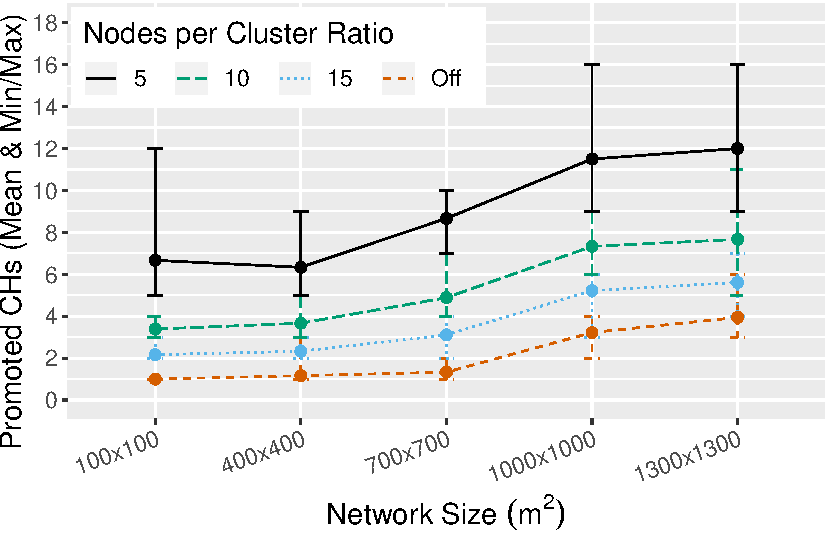
\includegraphics[width=0.49\textwidth, keepaspectratio]{figure/Results/ParameterEvaluation/MaxNodeCount_PromotedCHCount.pdf}
    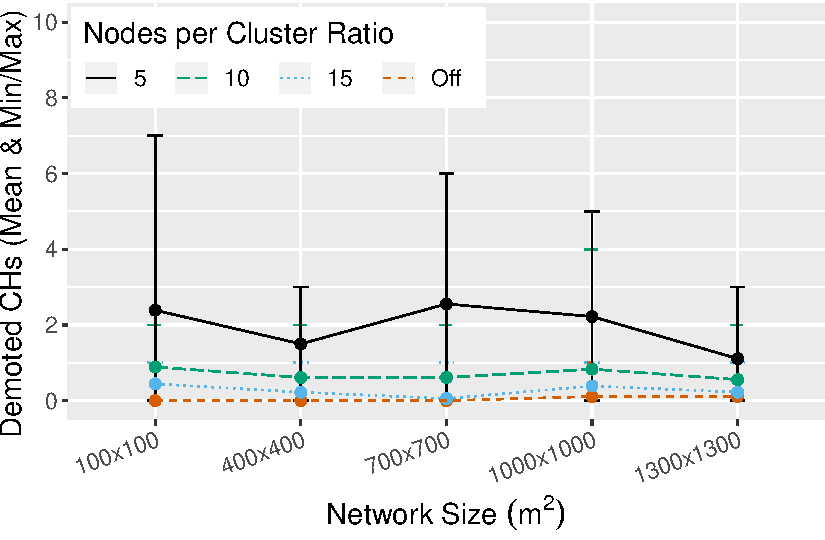
\includegraphics[width=0.49\textwidth, keepaspectratio]{figure/Results/ParameterEvaluation/MaxNodeCount_DemotedCHCount.pdf}
    \caption{The number of elected CHs before the Demote service runs, and the number of demoted CHs.}
    \label{fig:nodes-per-cluster-ratio-promoted-ch-count}
\end{figure}

\section{Comparing \atwo{} with Clustering}
\label{sec:comparing-a2-and-clustering}
In this section, we show the results of evaluating our clustering implementation and compare with the results from our evaluation of the original \atwo{} system. We show results for stability, reliability, latency, and estimated energy usage for all tests we run. We use different parameter values for some network topologies during this comparison. The most significant change is that we increase the competition radius as the network sizes increases. We list all parameter values for these tests in \cref{app:parameter-values-for-the-atwo-comparison}.


\subsection{Reliability and Stability}
\label{subsec:evaluation-reliability}
\begin{newtext}
We show reliability and stability for the evaluations with 50 nodes in \cref{subfig:reliability-50-nodes} and for 200 nodes in \cref{subfig:reliabilty-200-nodes}. Looking at the reliability for both of these, we see almost no difference for most network topologies, except with 50 nodes for 2200x2200 and 2500x2500 $m^2$, where the reliability drops when using clustering. The reason it drops is presented in detail \cref{subsec:competition-radius}, but essentially, too small clusters are created for these sparse networks.

However, the stability results have a higher variance. In the networks with 50 nodes, the clustered networks have lower stability, there are some tests which achieve similar levels of stability, but on average it is lower or much lower. In networks with 200 nodes, on the other hand, clustering achieves better results, the average stability is still lower than for the \atwo{} system, but there are some tests where clustering outperforms \atwo{} slightly. 

The reason \atwo{} drops in stability for 200 nodes, is that when one node loses connection with the network, the whole network has to spend on average, two or three rounds running the Join service. The clustering implementation, on the other hand, should only have to run the Join service locally in the affected cluster, which impacts stability less. However, since the clustering implementation lacks fault tolerance (discussed in \cref{section:evaluation-discussion}), the stability results for clustering are worse than they could be.

Furthermore, the stability has a decreasing trend in the 50 node networks while it is increasing in the 200 node networks. The reason the stability has an increasing trend in 200 node networks is that the small networks are dense and therefore generate more interference, which increases the number of faults that occur. However, we have not tested larger networks than 1300x1300 $m^2$ using 200 nodes, and it is possible that the stability will show a similar trend as the 50 nodes network when the area of the networks is increased further.

\end{newtext}
\begin{figure}[bt]
    \centering
    \begin{subfigure}{\textwidth}
            \centering
            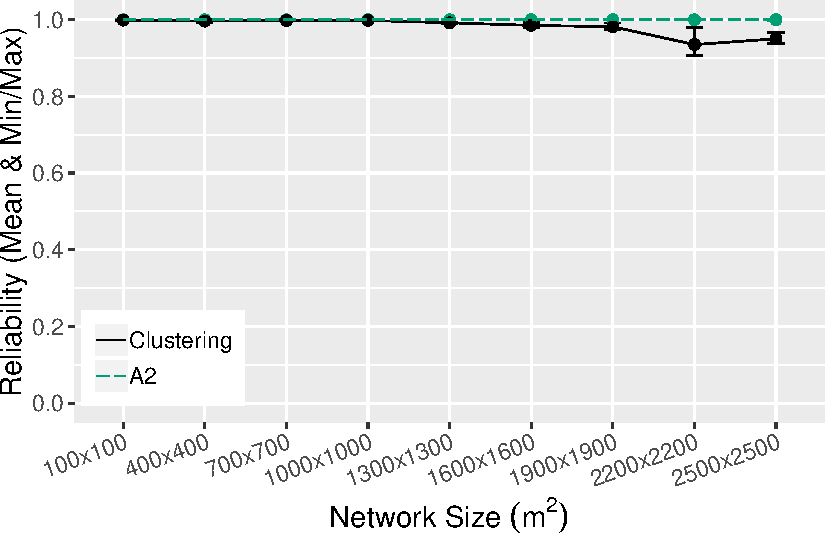
\includegraphics[width=0.45\textwidth]{figure/Results/ChaosComparison/ChaosComparison_50_Reliability.pdf}
            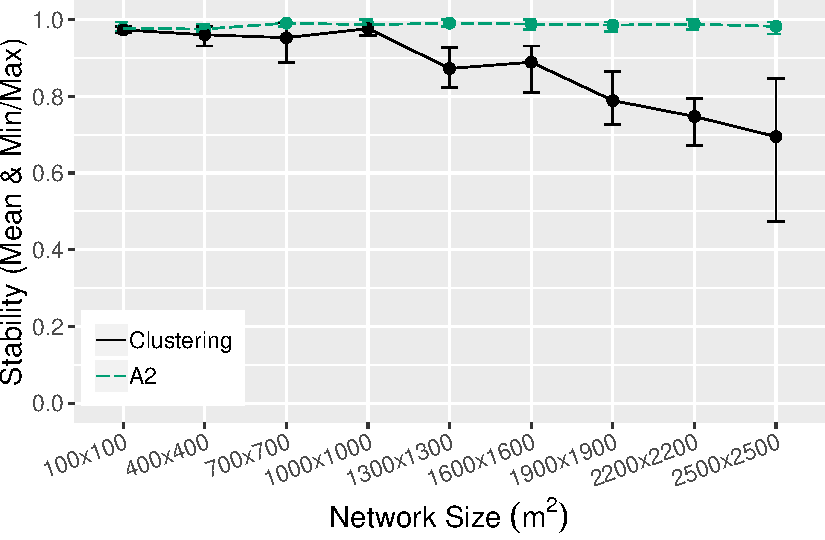
\includegraphics[width=0.45\textwidth]{figure/Results/ChaosComparison/ChaosComparison_50_Stability.pdf}
            \caption{Networks with 50 nodes.}
            \label{subfig:reliability-50-nodes}
    \end{subfigure}
    \hfill
    \begin{subfigure}{\textwidth}
        \centering
        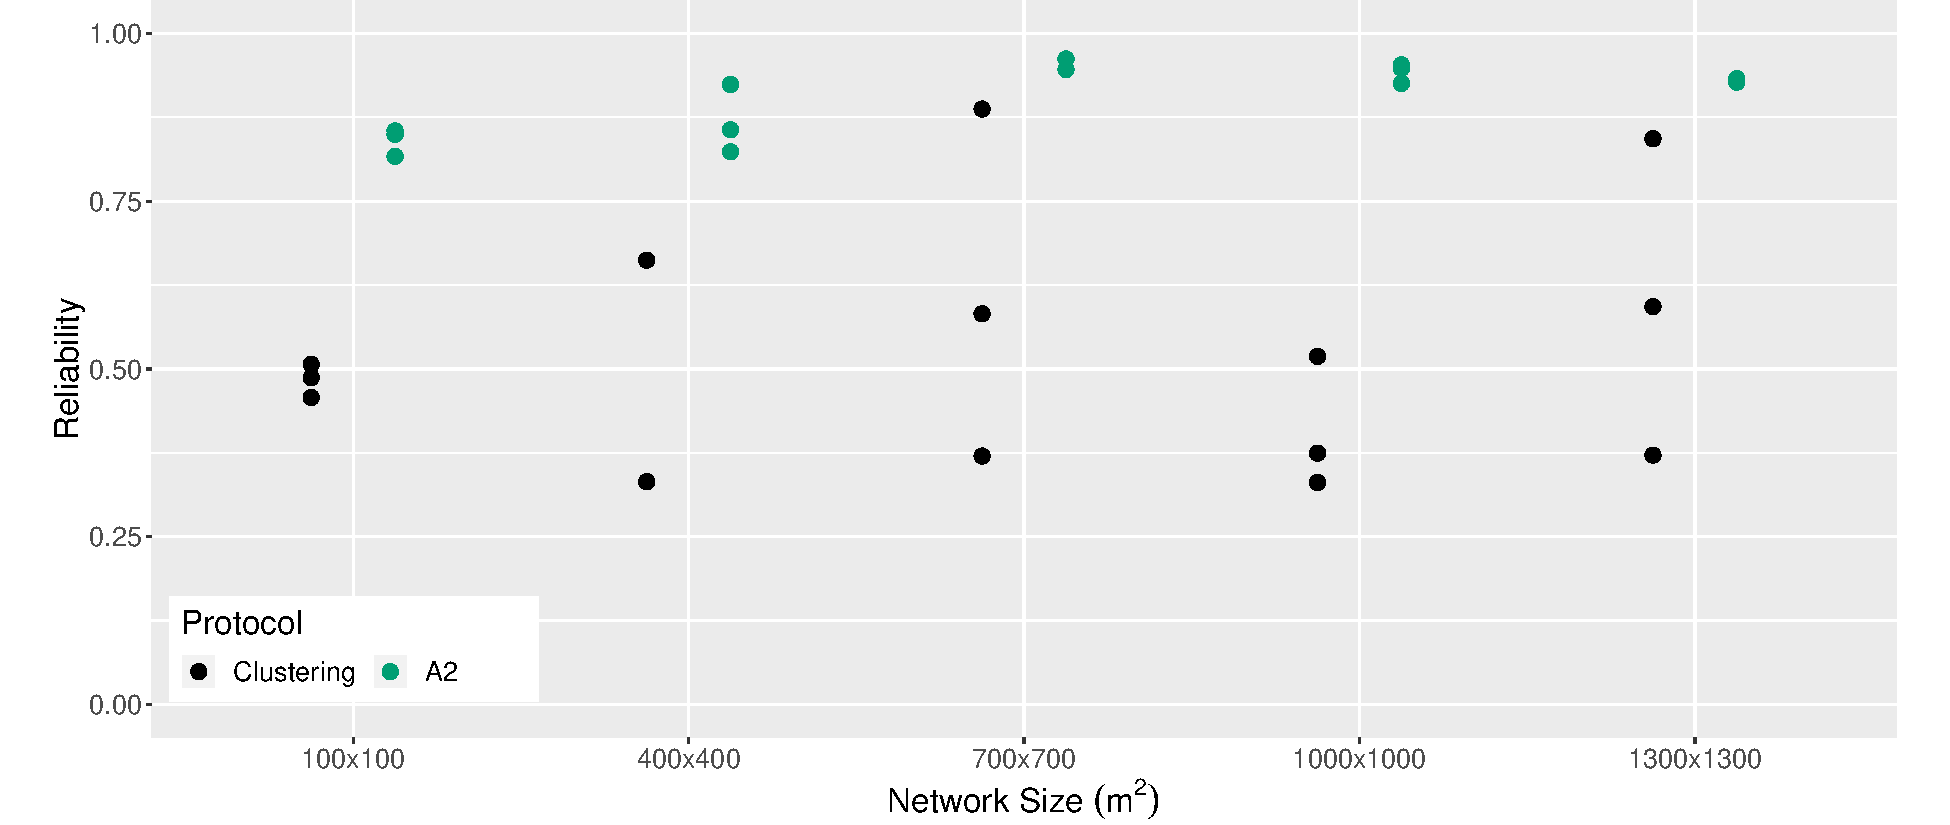
\includegraphics[width=0.45\textwidth]{figure/Results/ChaosComparison/ChaosComparison_200_Reliability.pdf}
        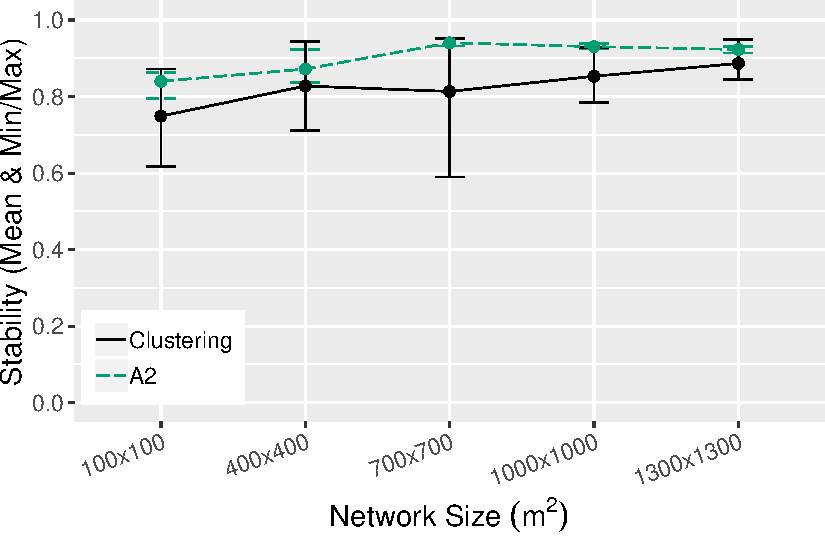
\includegraphics[width=0.45\textwidth]{figure/Results/ChaosComparison/ChaosComparison_200_Stability.pdf}
        \caption{Networks with 200 nodes.}
        \label{subfig:reliabilty-200-nodes}
    \end{subfigure}
    \caption{Reliability and stability comparison between \atwo{} with clustering and original \atwo{}.}
    \label{fig:reliability-result}
\end{figure}



\begin{figure}[bt]
    \centering
    \begin{subfigure}{0.45\textwidth}
        \centering
        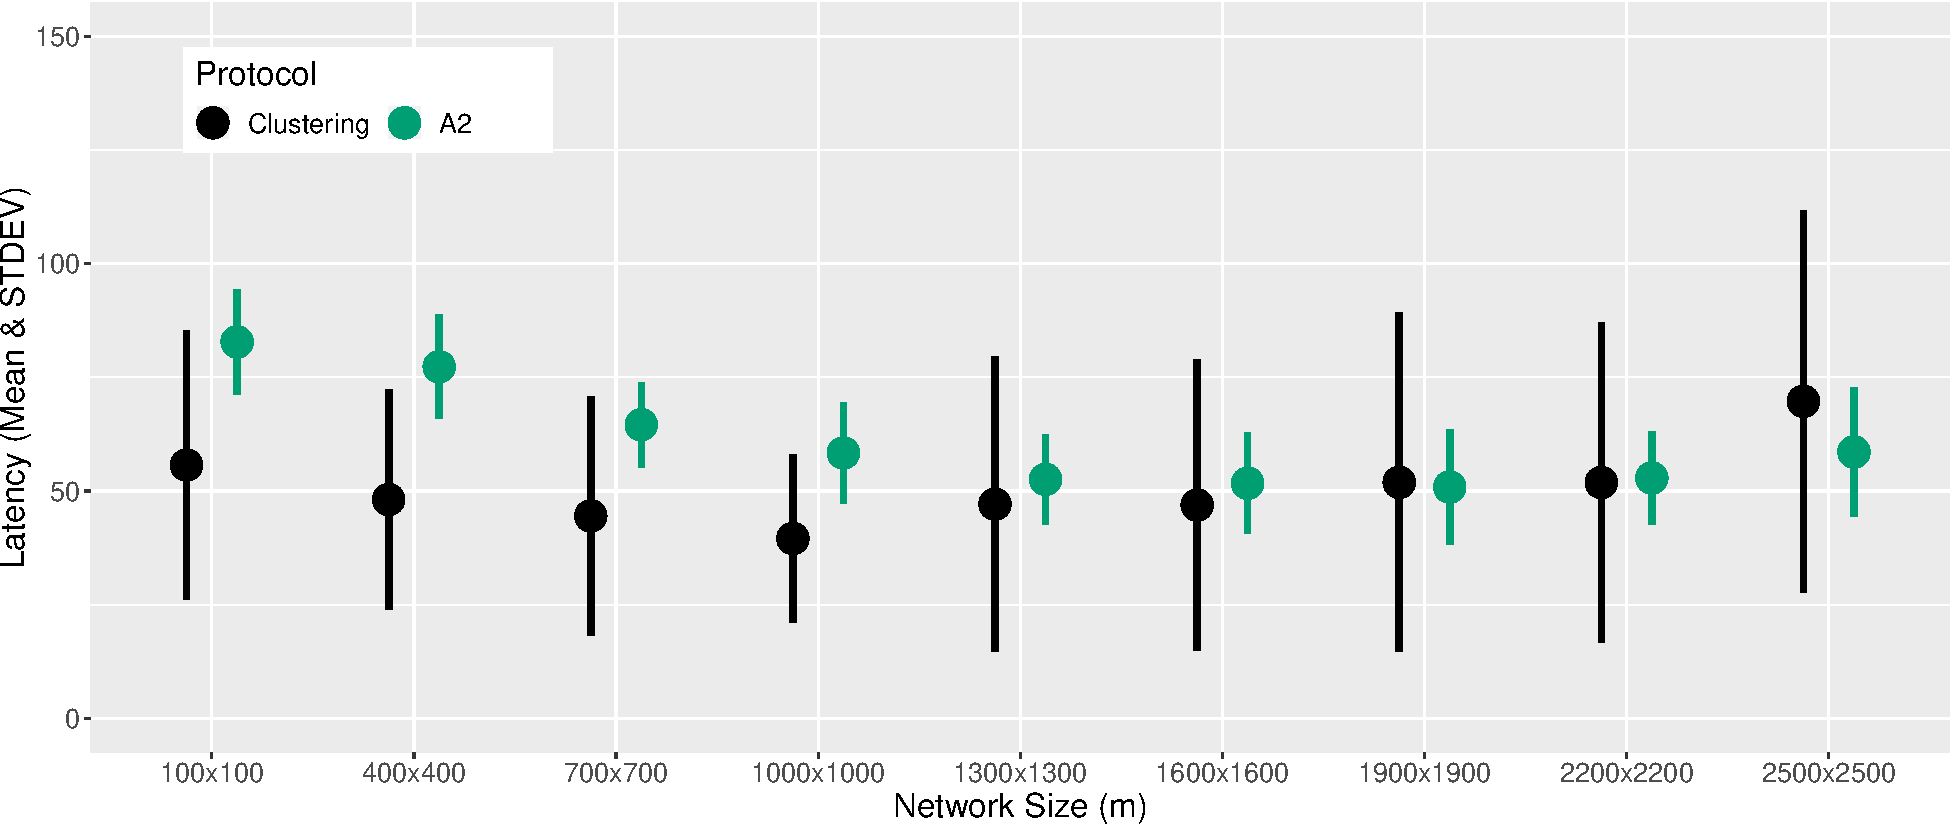
\includegraphics[width=\textwidth]{figure/Results/ChaosComparison/ChaosComparison_50_Latency.pdf}
        \caption{Networks with 50 nodes.}
        \label{subfig:latency-50-nodes}
    \end{subfigure}
    %\hfill
    \begin{subfigure}{0.45\textwidth}
        \centering
        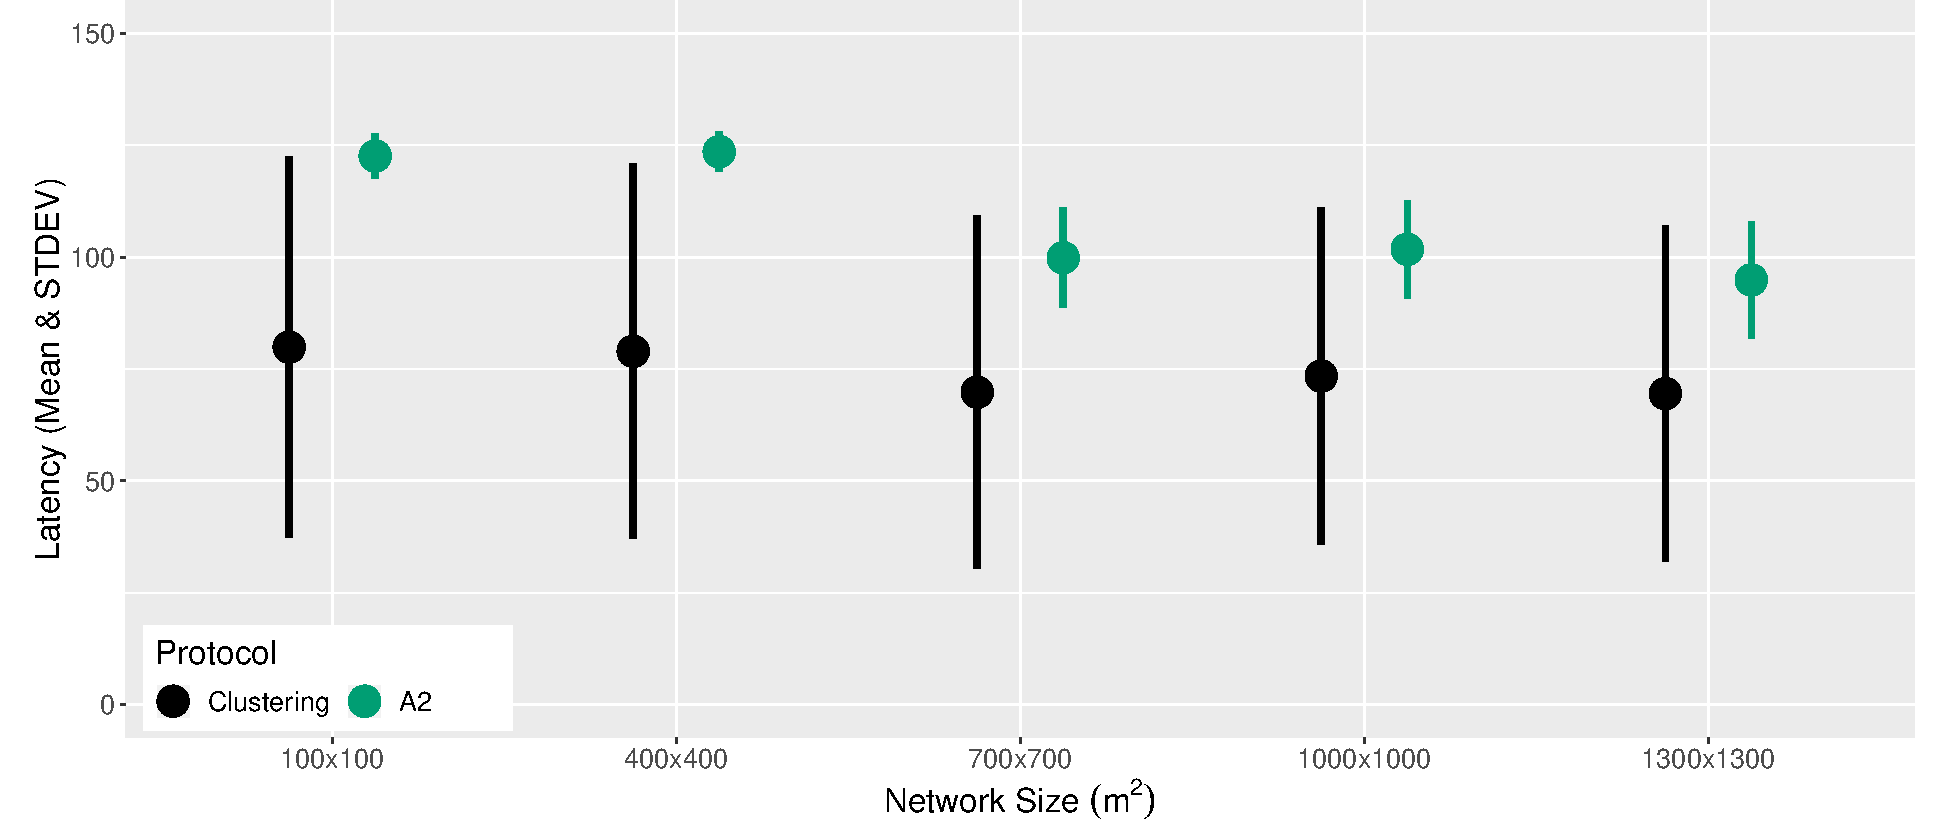
\includegraphics[width=\textwidth]{figure/Results/ChaosComparison/ChaosComparison_200_Latency.pdf}
        \caption{Networks with 200 nodes.}
        \label{subfig:latency-200-nodes}
    \end{subfigure}
    \caption{Latency comparison between \atwo{} with clustering and original \atwo{}.}
    \label{fig:latency-results}
\end{figure}


\subsection{Latency}
We show the mean latency and standard deviation for each test we run in \cref{fig:latency-results}. Looking at the tests using 50 nodes (\cref{subfig:latency-50-nodes}) the latency for the clustering implementation is on average a little lower for network topologies smaller than $2200x2200m^2$, after that the \atwo{} system outperforms our implementation. However, for all network topologies our clustering implementation has a higher standard deviation. We see a similar trend for 200 nodes (\cref{subfig:latency-200-nodes}), the standard deviation is still high; however, our clustering implementation consistently has a lower mean latency for all topologies tested. 

If we compare the latency between 50 nodes and 200 nodes, we see that it increases as the number of nodes increases. Consequently, we get lower latency when applying clustering since each cluster only contains a proportion of all nodes in the network.



\begin{figure}[bt]
    \centering
    \begin{subfigure}{0.45\textwidth}
        \centering
        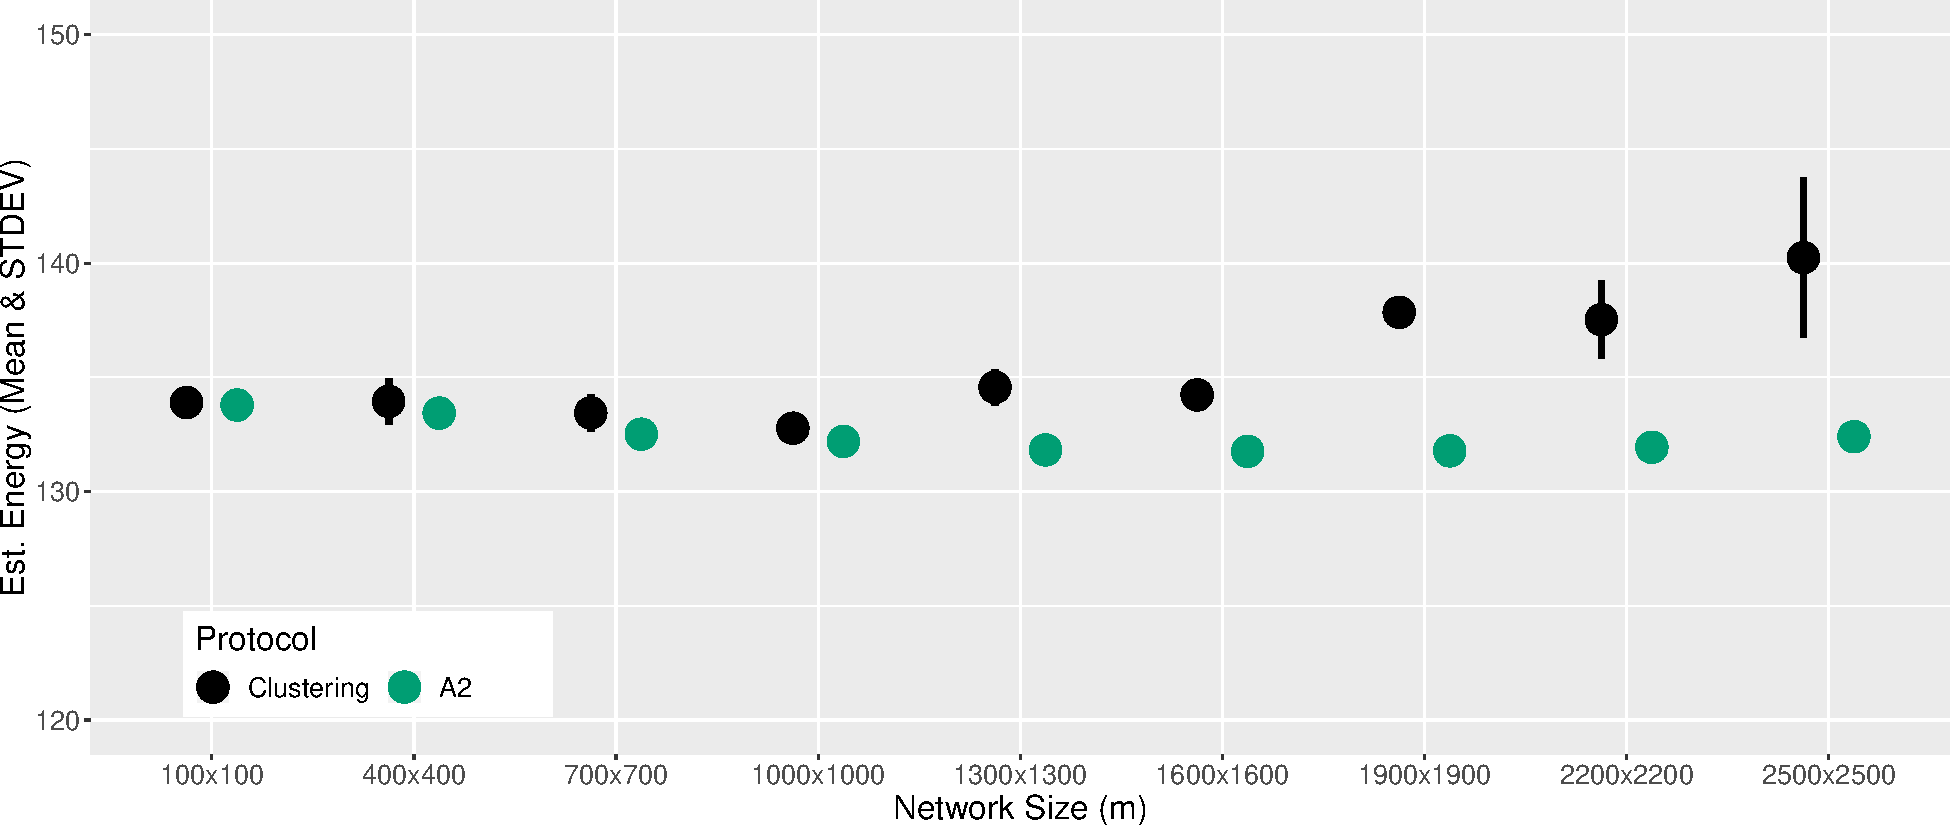
\includegraphics[width=\textwidth]{figure/Results/ChaosComparison/ChaosComparison_50_Energy.pdf}
        \caption{Networks with 50 nodes.}
        \label{subfig:energy-50-nodes}
    \end{subfigure}
    \begin{subfigure}{0.45\textwidth}
        \centering
        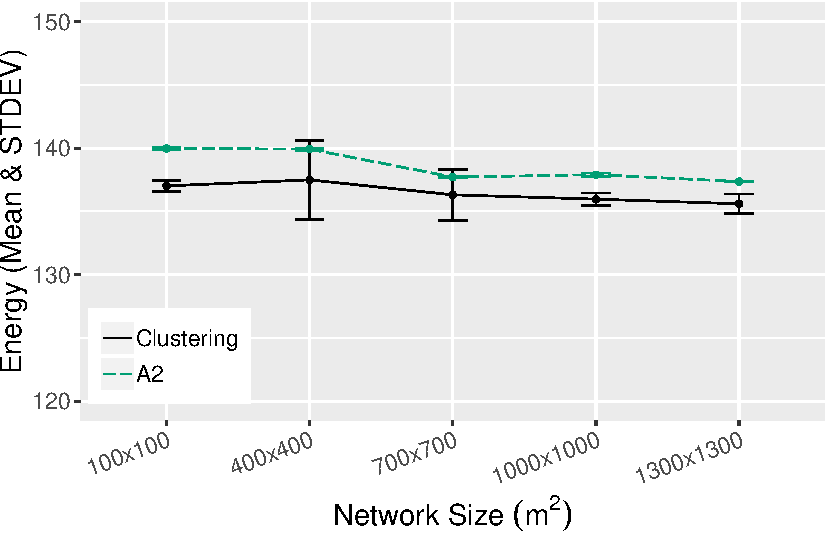
\includegraphics[width=\textwidth]{figure/Results/ChaosComparison/ChaosComparison_200_Energy.pdf}
        \caption{Networks with 200 nodes.}
        \label{subfig:energy-200-nodes}
    \end{subfigure}
    \caption{Energy comparison between \atwo{} with clustering and original \atwo{}.}
    \label{fig:energy-results}
\end{figure}


\subsection{Energy}
In \cref{fig:energy-results}, we show the mean energy usage per node per Energest time unit. We observe in \cref{subfig:energy-50-nodes} that energy usage for clustering increases with network area. We also observe that stability (\cref{subfig:reliabilty-200-nodes}) has an inverse relationship to energy usage, because an unstable node consumes more energy than a stable node. Both associating with the network and running the Join service requires more energy than the max application. They take more energy since the Join service takes longer time than the max application, and when a node associates it does not sleep.

Comparing 50 to 200 nodes we notice a higher energy usage on average for 200 nodes, which we expect to see since more nodes require more communication and longer rounds, which leads to higher energy consumption. Clustering shows a small advantage with 200 nodes \cref{subfig:energy-200-nodes}, compared to \atwo{}; each cluster can reach consensus in fewer slots than the whole network can, which is why the average energy usage is lower on all topologies.

Finally, the energy usage differs from the other metrics in that it is measured during both the coordination and application phase.  It is measured in all rounds because the energy results for only the applications could be misleading since the energy usage by the clustering process could outweigh the benefit of clustering the network.

\begin{figure}[bt]
    \centering
    \begin{subfigure}{0.24\textwidth}
        \centering
        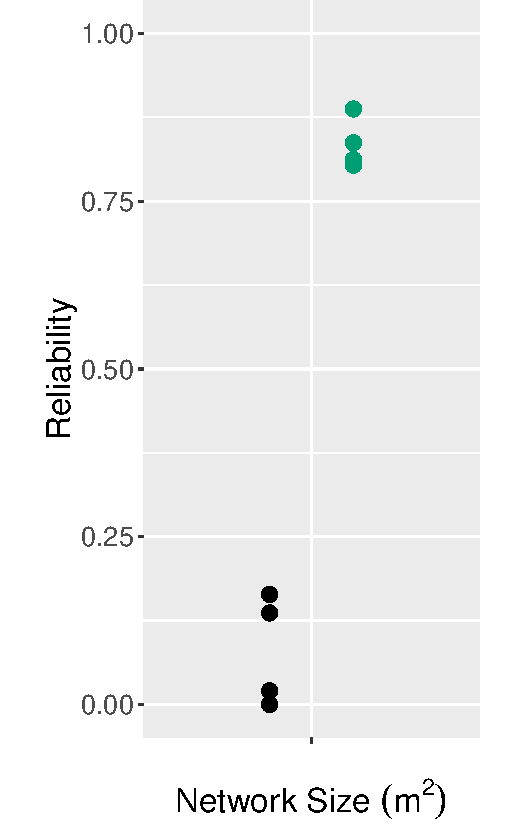
\includegraphics[width=\textwidth, keepaspectratio]{figure/Results/ChaosComparison/Flocklab/FlocklabComparison_Reliability.pdf}
        \caption{Reliability.}
        \label{subfig:flocklab-reliability}
    \end{subfigure}
    \begin{subfigure}{0.24\textwidth}
        \centering
        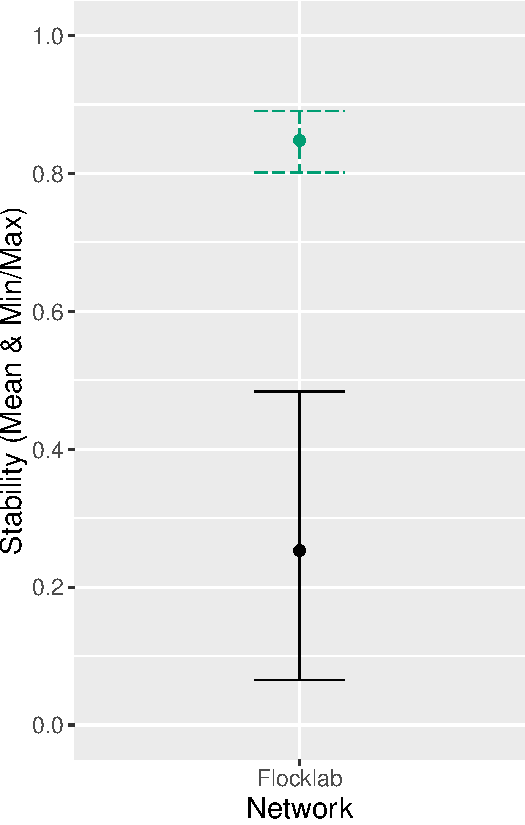
\includegraphics[width=\textwidth, keepaspectratio]{figure/Results/ChaosComparison/Flocklab/FlocklabComparison_Stability.pdf}
        \caption{Stability.}
        \label{subfig:flocklab-stability}
    \end{subfigure}
    \begin{subfigure}{0.24\textwidth}
        \centering
        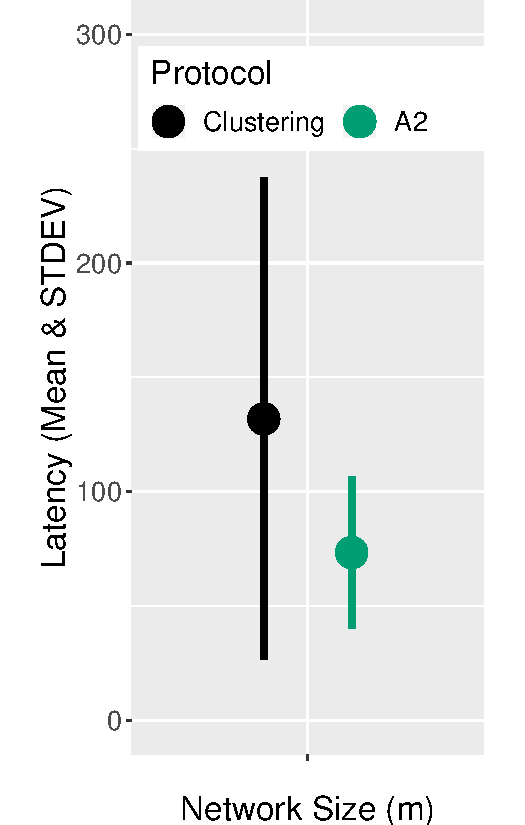
\includegraphics[width=\textwidth, keepaspectratio]{figure/Results/ChaosComparison/Flocklab/FlocklabComparison_Latency.pdf}
        \caption{Latency.}
        \label{subfig:flocklab-latency}
    \end{subfigure}
    \begin{subfigure}{0.24\textwidth}
        \centering
        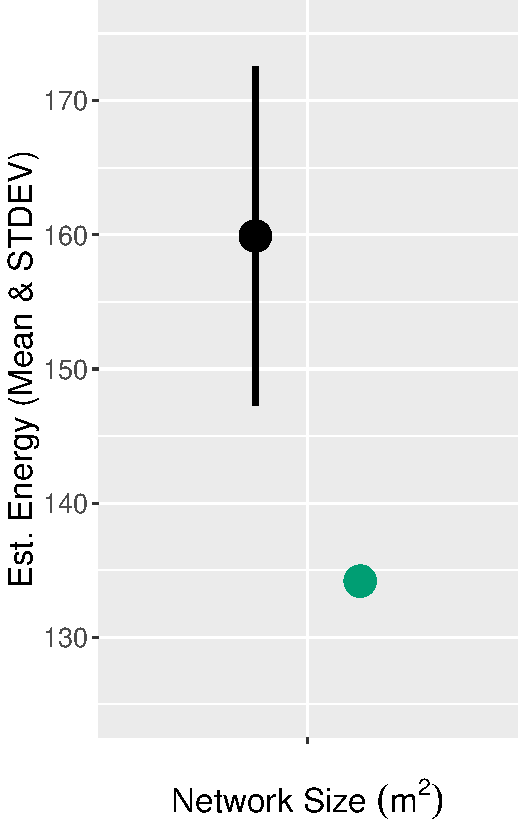
\includegraphics[width=\textwidth, keepaspectratio]{figure/Results/ChaosComparison/Flocklab/FlocklabComparison_Energy.pdf}
        \caption{Energy.}
        \label{subfig:flocklab-energy}
    \end{subfigure}
    \caption{The results of running \atwo{} and our clustering implementation on the Flocklab testbed. We show the mean and min/max for stability and reliability, and the mean and standard deviation for latency and energy consumption.}
    \label{fig:flocklab-results}
\end{figure}



\subsection{Flocklab}
We present the results from our tests on the Flocklab testbed in \cref{fig:flocklab-results}, which we get by running our clustering implementation and the \atwo{} system four times each. We see that \atwo{} outperforms our implementation in all metrics, achieving higher reliability and stability, lower latency, and lower energy consumption.

\begin{newtext}
Flocklab is a small and relatively sparse network with only 27 nodes, and it is also affected by external interference, which the simulations do not model. All of these factors contribute to lower stability, for both \atwo{} and the clustering implementation. 

When clustering the Flocklab network what often happens is that some node loses connection and need to associate with the network, to handle this the Join service is scheduled. Because no test run created more than two CHs, approximately half of the nodes begins to run the Join service, this makes it even harder for the other nodes to communicate, forcing more nodes to associate, creating a compounding effect of more and more nodes associating with the network. Nonetheless, running the clustering implementation on the Flocklab testbed demonstrates that the clustering process works when running on real nodes.
\end{newtext}


\section{Discussion}
\label{section:evaluation-discussion}
In this section, we discuss insights from our results. Furthermore, we discuss how our limitation on fault tolerance affected the stability of the networks. We also discuss running other applications in a clustered network, and end with some comments regarding the scalability and energy efficiency of a clustered network.


\subsection{Stability and Fault Tolerance}
\label{subsec:discussion-stability-and-fault-tolerance}
\begin{newtext}
From the results we get from comparing \atwo{} to our implementation, we see that our clustering implementation achieves similar reliability in almost all cases. However, the stability has high variance and is, in some cases, much lower. The primary reason for these stability results is that we did not consider fault tolerance for our clustering implementation. In this section, we will describe and discuss what scenarios lead to lower stability and how they relate to fault tolerance.



One of the most common fault tolerance issues is that a node loses connection to the network and has to re-associate with it. For a node, this process should look as follows.
    
\begin{enumerate}
    \item A node does not receive any packet for some rounds equal to \emph{round re-synchronisation threshold}.
    \item The node switches to association, listening for a packet with which it can synchronise.
    \item The node sets the join flag in outgoing packet headers, requesting that the initiator schedule the Join service.
    \item The current initiator schedules the Join service for its cluster.
\end{enumerate}

By analysing the tests from the comparison of our implementation to the \atwo{} system, we see that stability issues always occur in step 4 of this process. We performed this analysis by looking at the outcomes of tests in the simulator; we do not attach any details of this here since it is too extensive.

Properly scheduling the Join service is complicated since we change both which node is the initiator and which nodes communicate while switching between cluster and cluster head rounds. The most common scenario, exemplified in \cref{fig:scenario-one-bug-example}, is that a node, in this case node 17, sets its join flag during a CH round, this happens first in round 270 in the example, and forces the first CH to schedule the Join service. The problem is that it does not matter which cluster node 17 has joined, it is always the first cluster that schedules the Join service. Consequently, since node 17 never gets the chance to join, because the wrong cluster is running the Join service, this scenario continues until a reclustering is scheduled.

\end{newtext}
\begin{figure}[bt]
    \centering
    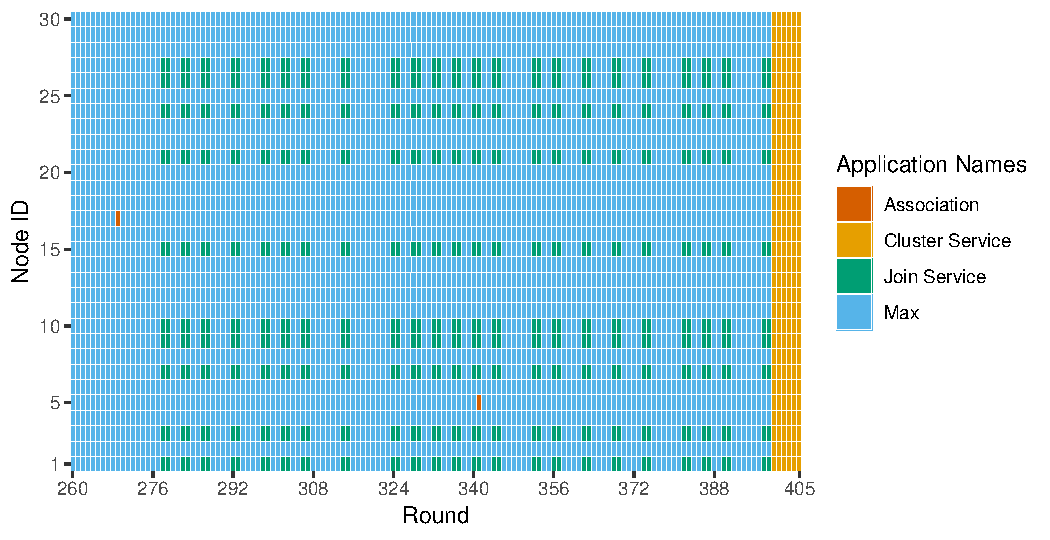
\includegraphics[width=0.75\textwidth] {figure/Results/Discussion/50NodesRun21000x1000Scenario1Example.pdf}
    \caption{Example of what happens when a node requests the Join service to be scheduled, blue is the correct application, green is the Join service, and yellow is the Clustering service. The first cluster repeatedly schedules the Join service without any effect.}
    \label{fig:scenario-one-bug-example}
\end{figure}


\begin{newtext}
Furthermore, if a CH loses connection to the network and has to associate, additional problems can occur. What happens depends on which CH associates. First, if the CH with the lowest ID associates, the network cannot continue normal execution, since that CH is the initiator during CH rounds. Causes and solutions to this problem are discussed more thoroughly in \cref{subsec:implementation_discussion-the-initiator}. Second, if another CH associates, the network will continue to execute the application. However, that node neither contributes its value nor sets its flag during CH rounds, which means the other nodes will never know that they have reached completion and cannot shut down early during CH rounds. This scenario does not impact the stability of the application, but it increases the latency and energy usage.

Finally, that our clustering implementation works in the absence of faults is supported by the reliability and stability results in \cref{fig:reliability-result}. Since the reliability metric does not include scenarios which require fault tolerance, it expresses the fact that clustering achieves good results during normal operation of the network. Additionally, from the stability results for 200 nodes, \cref{subfig:reliabilty-200-nodes}, we see that there are some tests which achieve better stability than \atwo{}, demonstrating that our clustering implementation has the potential to achieve better stability than the \atwo{} system in larger networks.
\end{newtext}


\subsection{Clustering Parameters}
\label{discussion:clustering-parameters}
The results we see in the parameter evaluation varies greatly, both when looking at a single test but also when looking at the different evaluations of the parameters combined. From the parameter evaluation, we can give some general remarks about each of the parameters.

\begin{newtext}
%Resync threshold discussion.
As we see in the resynchronisation threshold evaluation (\cref{subsec-resync-threshold}), both the stability and reliability increase significantly as the re-sync threshold increases. These results suggest that we should increase the re-sync threshold indefinitely. We did not evaluate this parameter further due to time constraints.


However, there are other reasons why indefinitely increasing this parameter will not yield the desired results. Re-sync threshold controls the number of rounds a node will wait while receiving no packets until it re-synchronises with the network again. Thus this parameter only fixes the symptom and not the cause of the problem, which is that a node has a bad connection to its cluster. For example, with a high re-sync threshold a node might stay in a suboptimal cluster since it receives enough packets to reset the re-sync threshold but not enough packets to complete the application running in the cluster, which will affect reliability.
\end{newtext}


For competition radius, we see that it is a parameter useful for creating reliable clusters since it had the most significant impact on the stability of a test for larger network areas.

For minimum cluster size, the results we got suggest that this parameter has a small impact on the overall stability. However, we see no correlation between the overall number of CHs and the stability, suggesting that these results either have some other underlying cause or the difference is due to noise. However, this parameter should be used, since it prevents clusters with only one node to form.

Last, the nodes per cluster ratio parameter worked as we expected. With a lower value of this parameter, we saw that the clustering process created more CHs. However, this parameter requires careful consideration since it can cause too many CHs to be created for sparse networks, as we see in \cref{subsec:nodes-per-cluster-ratio}.

\subsection{Running Other Applications in a Clustered Network}
\label{subsec:discuss-other-apps}
\begin{newtext}
Throughout this thesis, we limit our evaluation to the Max application. This limitation is because our focus was to implement clustering on top of the \atwo{} system, and not to see how different applications perform in a clustered network. However, we discuss how other applications may benefit from a hierarchical network to show that clustering is not limited to the Max application. Some common applications for a WSN include calculating a sum, mean, median, or performing a 2 or 3 phase commit. However, running applications in a clustered network require some adaptations, compared to a normal network.

Calculating a sum in a clustered network requires few adaptations from an implementation for a non-clustered network, however, it can take advantage of the hierarchical communication. Each CH would be able to calculate its cluster's sum of proposed values. CHs then repeat the same process during the CH round where they share their intermediary sum with all other CHs. However, one difference when calculating a sum compared to a maximal value is that a CH needs to maintain a list of all contributed values and which node contributed with what value. If the nodes were to add values together, then the same value could be added to the sum multiple times. Since \atwo{} has a restriction on the packet size, the number of nodes that can propose values is restricted. Clustering the network would directly help with this since smaller parts of the network calculate separate sums, which means the list of proposed values is smaller.

Furthermore, calculating the median in a clustered network require more resources than calculating a sum, since all values have to be known to at least one node. Clustering affects the size of the required list in each cluster in the same way as when calculating the sum. However, the CH cannot perform an intermediary calculation as in the sum application. The CHs will instead share the lists between each other, merging all lists from all clusters, which would result in a list with a length equal to the number of nodes in the network. Therefore, calculating the median in a clustered network compared to a non-clustered network does not scale better with regards to packet size.

However, calculating the mean can make efficient use of a clustered network. A mean calculation requires two things: the sum of all proposed values, and the number of proposed values. Because a CH already knows the size of its cluster, they can perform a mean calculation in the same way as the sum calculation, with the extension that the CHs calculate the sum of the cluster sizes. At the end of the CH round, all CHs know the sum of all proposed values and the sum of all cluster sizes and can, therefore, calculate the mean.

Two other applications, which are more complicated than mean, sum and median, are two and three phase commit. Adapting these to run on a clustered network is not as straightforward. These applications can take advantage of clustering in all phases, running some of the collection and dissemination in parallel in every cluster. However, coordination is required between the CHs when switching between phases. The complexity lies in switching which node is the initiator when switching between inter- and intra-cluster communication. Especially if we were to implement a solution which executes the whole commit protocol in one round. We discuss the problems with switching between initiators in a round in \cref{subsec:implementation_discussion-the-initiator}.

In conclusion, clustering should increase the performance and scalability for many applications running on a WSN. Even applications which require a global view of the network can benefit from hierarchical communication. However, further work is required to implement these applications to evaluate the effectiveness of the clustering implementation.

\end{newtext}

\subsection{Achieving Better Scalability}
\begin{newtext}
One of the primary goals of this thesis is to increase the scalability of the \atwo{} system. We do not have a metric for measuring scalability directly, however, using the combined information from all metrics we argue that we achieved our goal. From the latency and energy usage results, we saw that our solution achieved a lower latency and energy usage for networks with 200 nodes. Additionally, since we cluster the network before running the Join service, the restriction caused by the flags field is not applied until after the clusters are created. Thus,  we increase the theoretical maximum number of nodes in the network, and the restriction is now local to every cluster.

However, there are some caveats to achieving better scalability. First, we measure the latency results per round. We do not take into account that a clustered network requires two complete rounds to agree on a global maximum value, while \atwo{} only requires one round. A clustered network requires two rounds because we schedule the inter- and intra-cluster communication in separate rounds. Second, even though our implementation has lower stability than \atwo{} in almost all cases, we achieve better latency and lower energy usage; this is good since we achieve those results even in the presence of more faults.

Furthermore, low stability could imply less scalability as well. Our results suggest that the stability decreases as the number of nodes increase, however, we have shown that this is caused by our limitation on fault tolerance and is not inherent to clustering the network.

Despite these caveats, we argue that the results are promising. From the discussion on fault tolerance we conclude that we could attribute the drops in stability to our limitation on fault tolerance. If future work research and implement fault tolerance, our clustering implementation has a high probability of achieving equal or better stability while running more scalable and energy efficient networks.
\end{newtext}


% CONCLUSION
\chapter{Conclusion}
\label{chap:conclusion}

In this thesis we introduced clustering to the \atwo{} protocol. The clustering algorithm is based on the HEED algorithm and uses a nodes residual energy to weigh its probability to announce itself as cluster head. We implemented clustering as a service in the \atwo{} Synchrotron, and evaluated our implementation in the Cooja simulator and on the Flocklab testbed looking at the metrics, reliability, latency, and energy consumption. Our results show that, on average, our clustering implementation performs significantly worse than \atwo{} when measuring the reliability. The energy consumption is similar and, for some tests, we achieve a lower latency than \atwo{}.



\section{Future Work}
\label{sec:future-work}
In this section, we list and discuss possible focuses of future work.


\subsection{Sleep Schemes}
Since forwarders do not contribute to the completion of the protocol, i.e., they do not set contribution flags. Sleep schemes are applicable to our clustering implementation since we showed in \cref{chap:evaluation} that using clustering does not increase the energy usage of the node in the network. Therefore, applying sleep schemes will directly improve energy preservation proportionally to the percentage of nodes put to sleep; this, however, could be in exchange for reliability. Sleep schemes are very applicable when using clustering and further work can research which nodes can be put to sleep, and how to determine which are crucial for keeping a network connected.

\subsection{Transmission Power}
In this thesis, all nodes have always used the same transmission power. It is conceivable to use a stronger transmission power for CHs that scales with competition radius, enabling all non CHs to sleep during CH rounds. If the few elected CHs use more power all other nodes, currently acting as forwarders, can all sleep and save energy. However, it would put a high requirement on dynamic clustering since CHs would need to be able to demote themselves. 


\subsection{Evaluating Stability}
In our evaluation we redefined the reliability metric slightly compared to Landsiedel et al.~\cite{chaos-introduction-paper}. We only consider reliability for the max application, and count other applications as an automatic failure, if they are run when not expected. In future evaluations, we could define reliability like Landsiedel et al.~does, the number of rounds in which the network reaches completion regardless of which application is running. Furthermore, we could also introduce a new metric called stability.

Stability could be a metric for how often a node requires resynchronisation. The measurement would describe, in the case of \atwo{}, how connected the network is; and in the case of clustering, how many times nodes switch between clusters. Comparing the stability metric between between these two could provide a better picture of the overall effectiveness of clustering a network.

\iffalse
%RE-SET CHAPTER COMMAND. OTHERWISE BIBLIOGRAPHY WILL BREAK.
\renewcommand{\chapter}{\svchapter}
\fi

% REFERENCES / BIBLIOGRAPHY
\cleardoublepage
\addcontentsline{toc}{chapter}{Bibliography}
% CREATED BY DAVID FRISK, 2016

\bibliographystyle{ieeetr}
\bibliography{include/backmatter/refs}

%\begin{thebibliography}{69}

%\bibitem{Reference} Frisk, D. (2016) A Chalmers University of Technology Master's thesis template for \LaTeX . Unpublished.

%\end{thebibliography}


% APPENDICES
\cleardoublepage
\appendix
\setcounter{page}{1}
\pagenumbering{Roman}			% Capitalized roman numbering starting from I (one)

% CREATED BY DAVID FRISK, 2016
\chapter{Appendix 1}
\label{app:a}
\section{Re-synchronization Latency Results}
\begin{figure}[H]
    
\centering
\begin{subfigure}{0.80\textwidth}
    \centering
    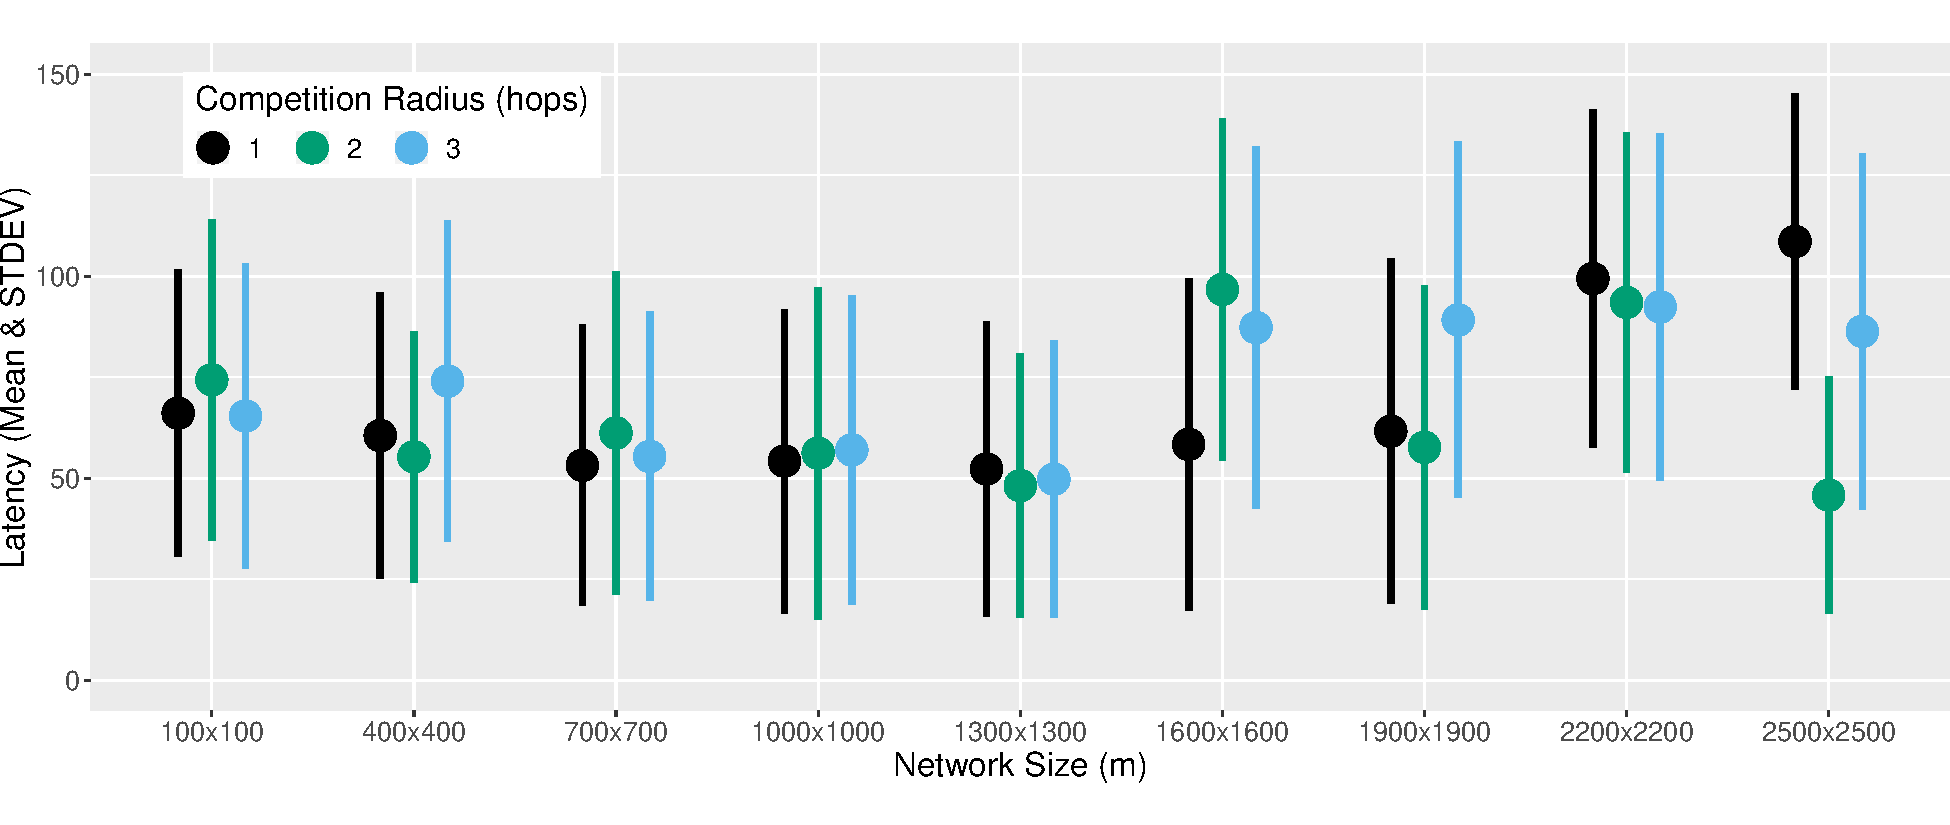
\includegraphics[width=\textwidth, keepaspectratio]{figure/Results/ParameterEvaluation/Latency/ResyncTreshold1_Latency.pdf}
    \caption{Re-synchronisation threshold 1.}
    \label{subfig:resync-treshold-1-latency}
\end{subfigure}
\begin{subfigure}{0.80\textwidth}
    \centering
    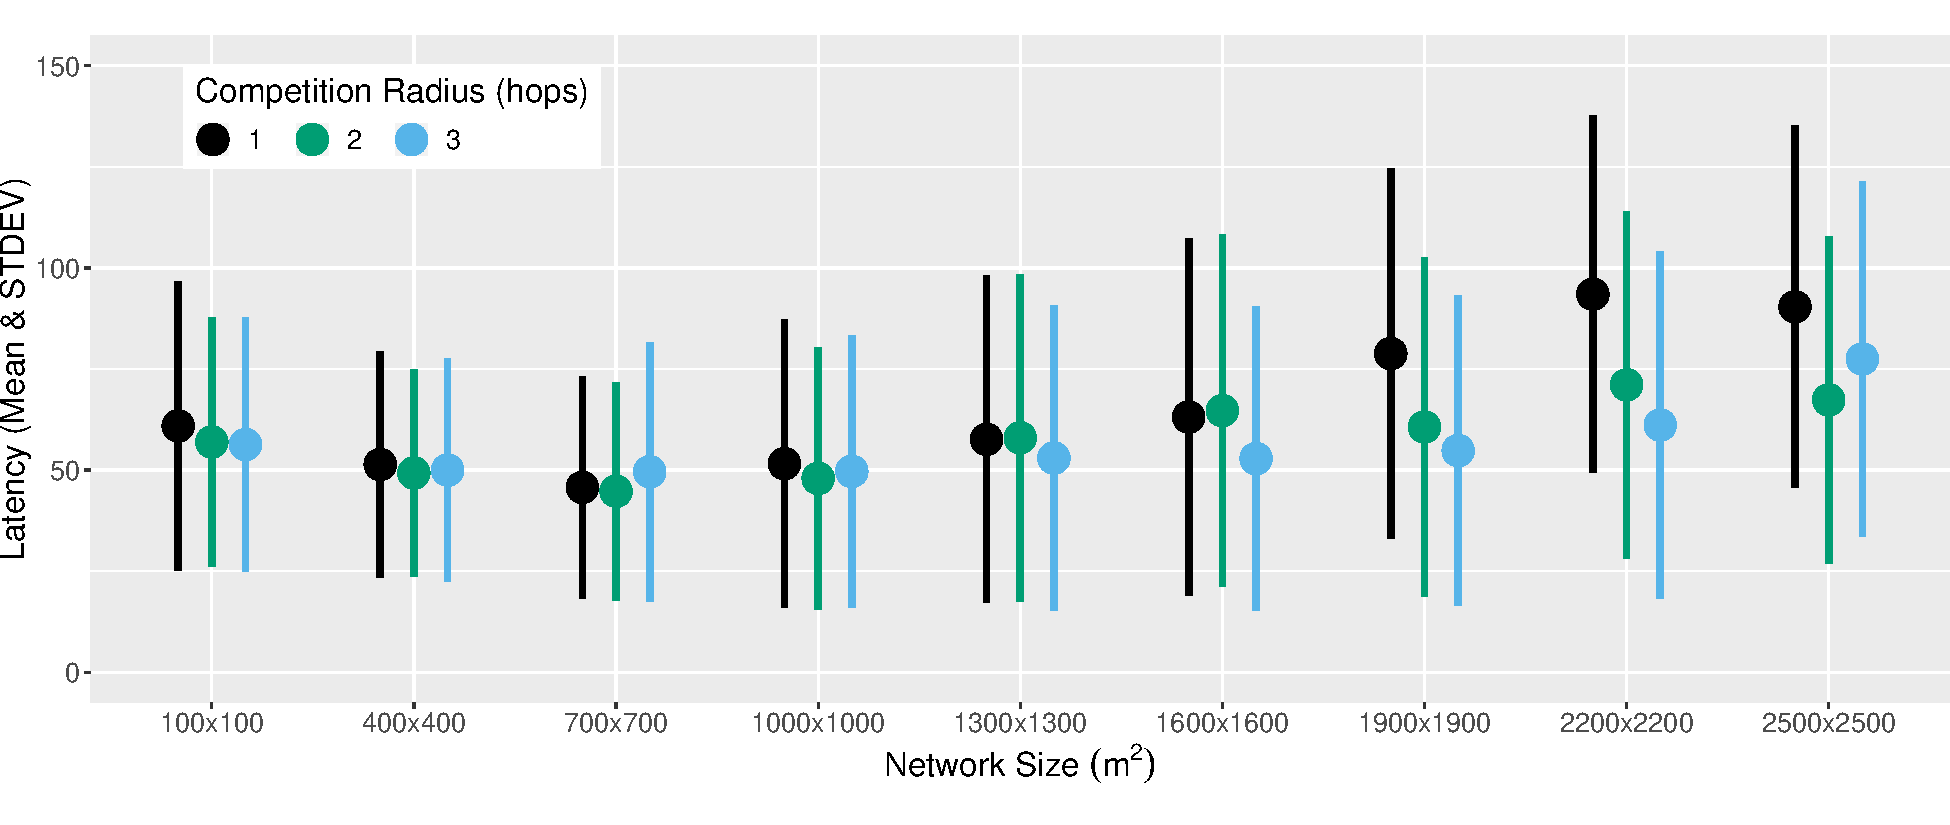
\includegraphics[width=\textwidth, keepaspectratio]{figure/Results/ParameterEvaluation/Latency/ResyncTreshold2_Latency.pdf}
    \caption{Re-synchronisation threshold 2.}
    \label{subfig:resync-treshold-2-latency}
\end{subfigure}
\begin{subfigure}{0.80\textwidth}
    \centering
    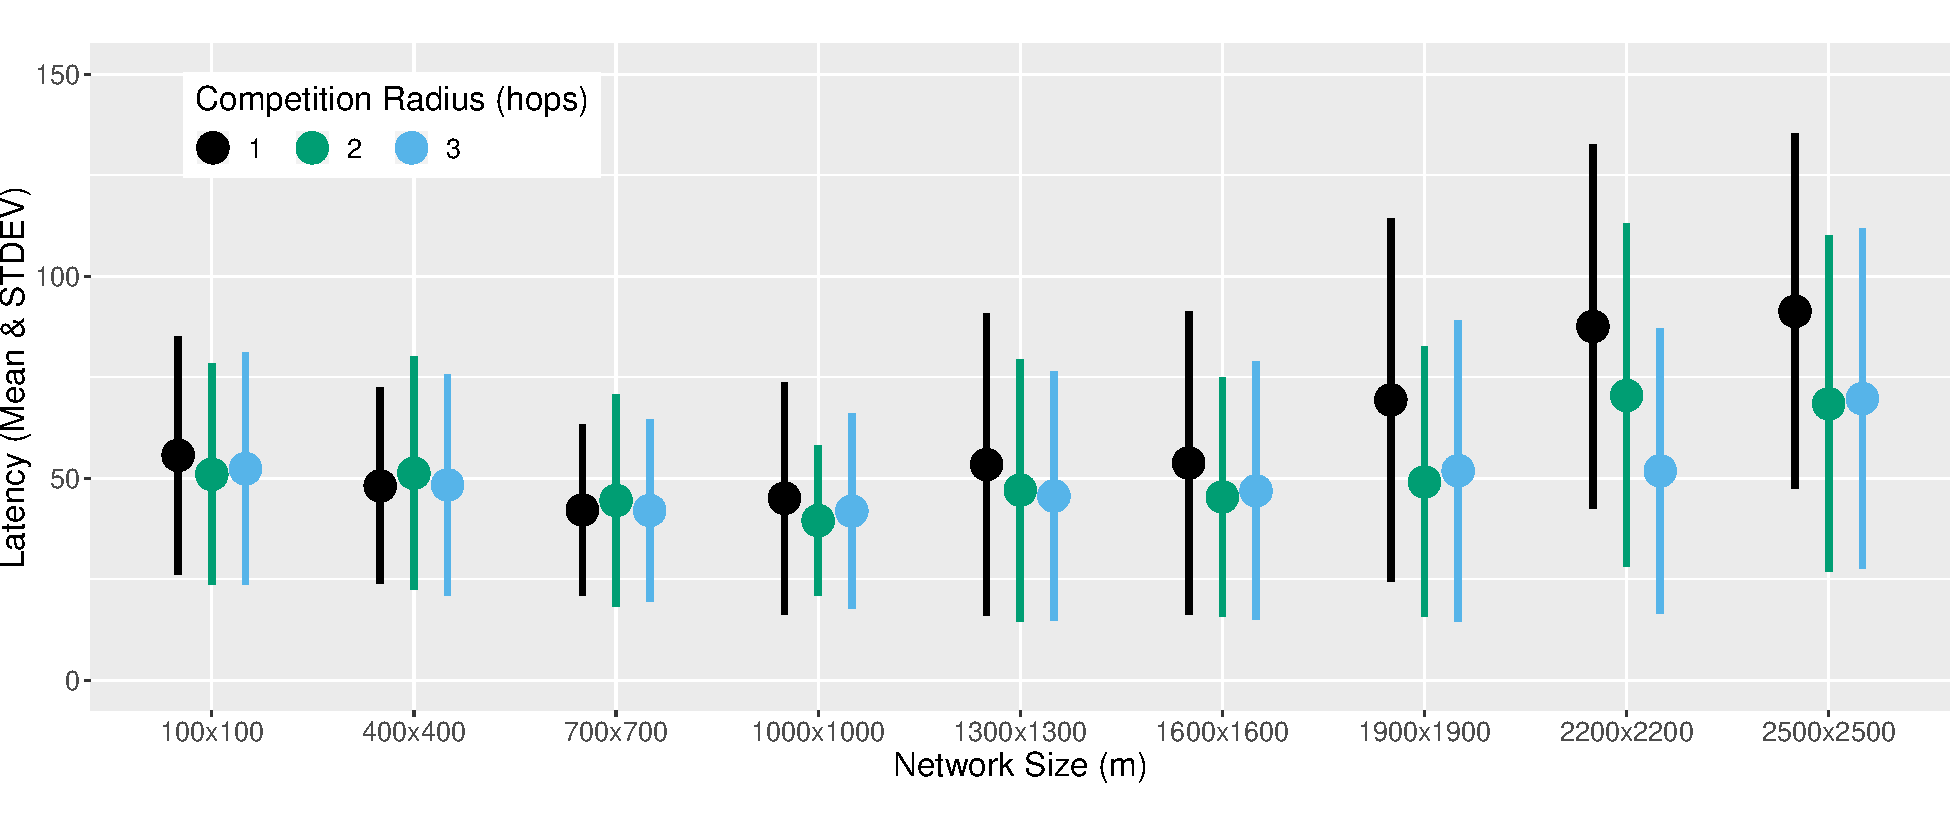
\includegraphics[width=\textwidth, keepaspectratio]{figure/Results/ParameterEvaluation/Latency/ResyncTreshold3_Latency.pdf}
    \caption{Re-synchronisation threshold 3.}
    \label{subfig:resync-treshold-3-latency}
\end{subfigure}

    \caption{Competition radii tests for different values of resynchronisation threshold.}
    \label{fig:resync-treshold-tests-latency}
\end{figure}

\section{Parameter Latency Plots}
\begin{figure}[H]
    
\centering
\begin{subfigure}{\textwidth}
    \centering
    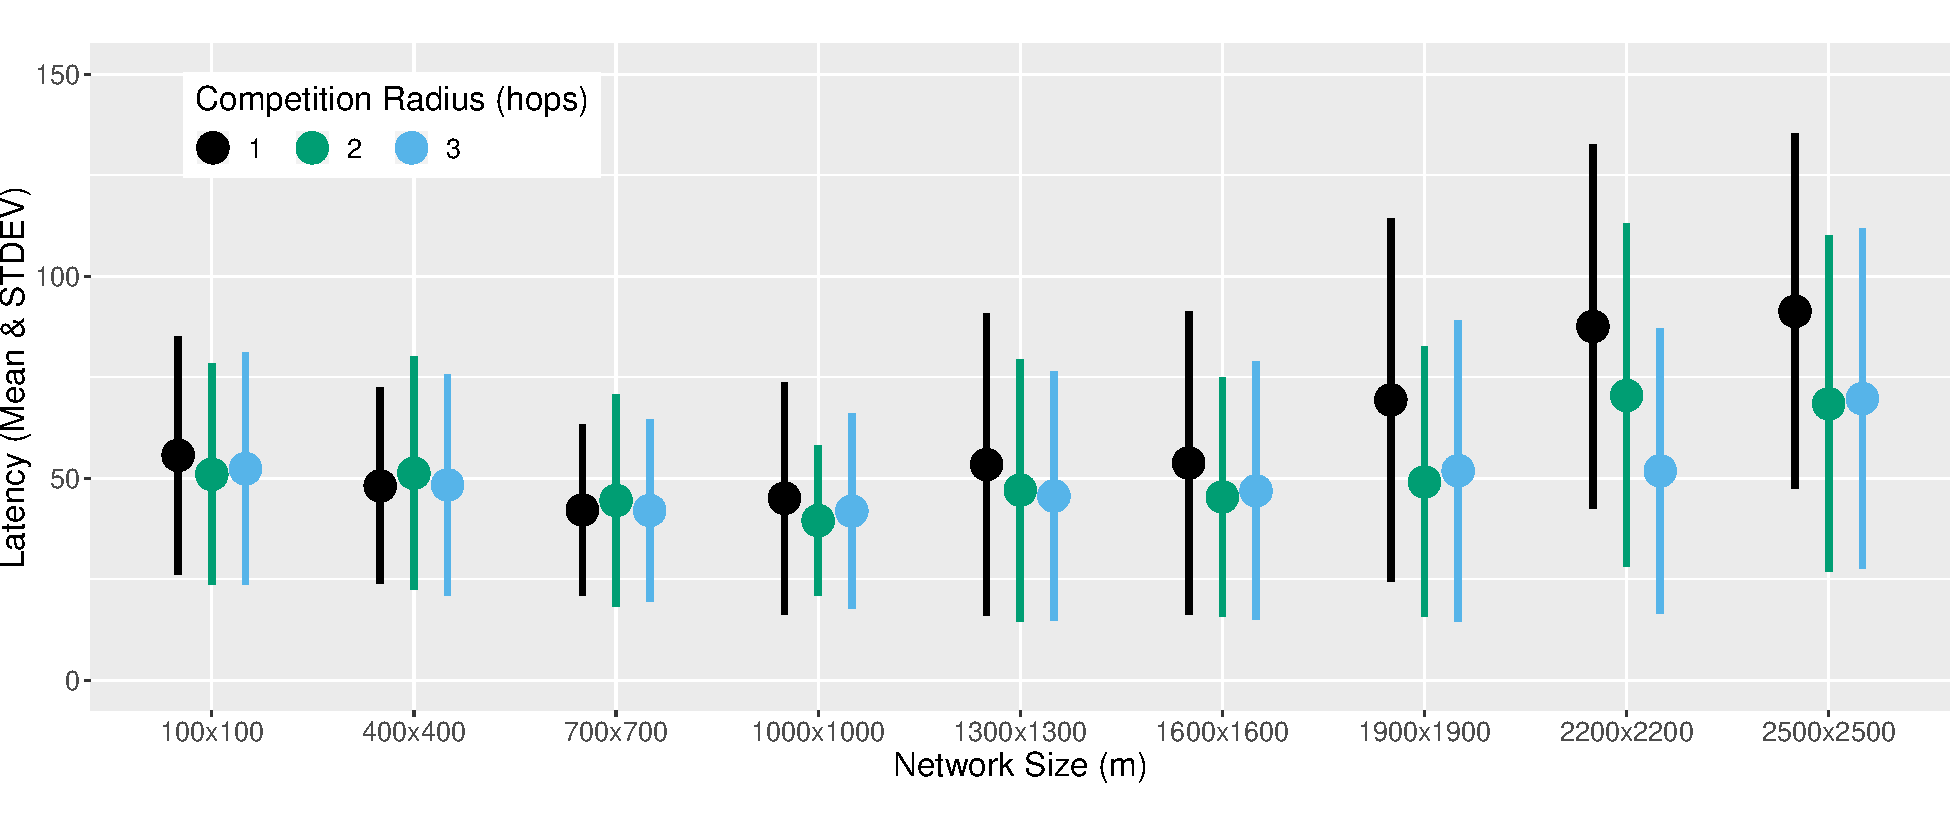
\includegraphics[width=\textwidth, keepaspectratio]{figure/Results/ParameterEvaluation/Latency/CompetitionRadius_Latency.pdf}
    \caption{Competition radius.}
    \label{subfig:competition-radius-latency}
\end{subfigure}
\begin{subfigure}{\textwidth}
    \centering
    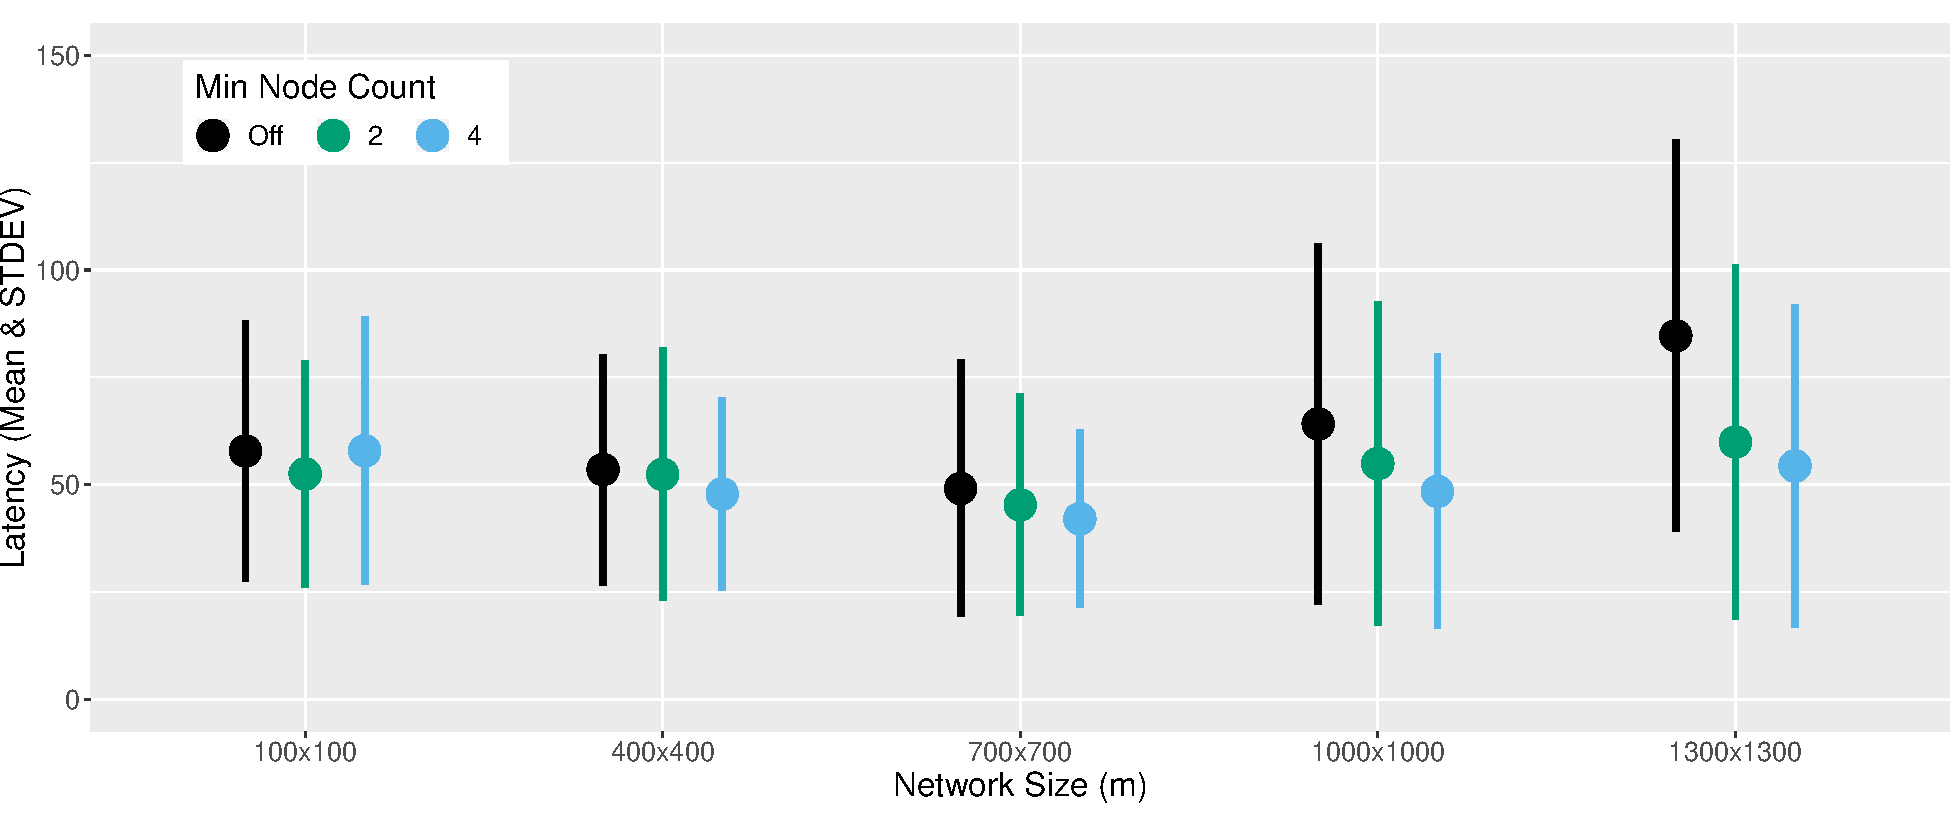
\includegraphics[width=\textwidth, keepaspectratio]{figure/Results/ParameterEvaluation/Latency/MinNodeCount_Latency.pdf}
    \caption{Minimum node count.}
    \label{subfig:min-node-count-latency}
\end{subfigure}
\begin{subfigure}{\textwidth}
    \centering
    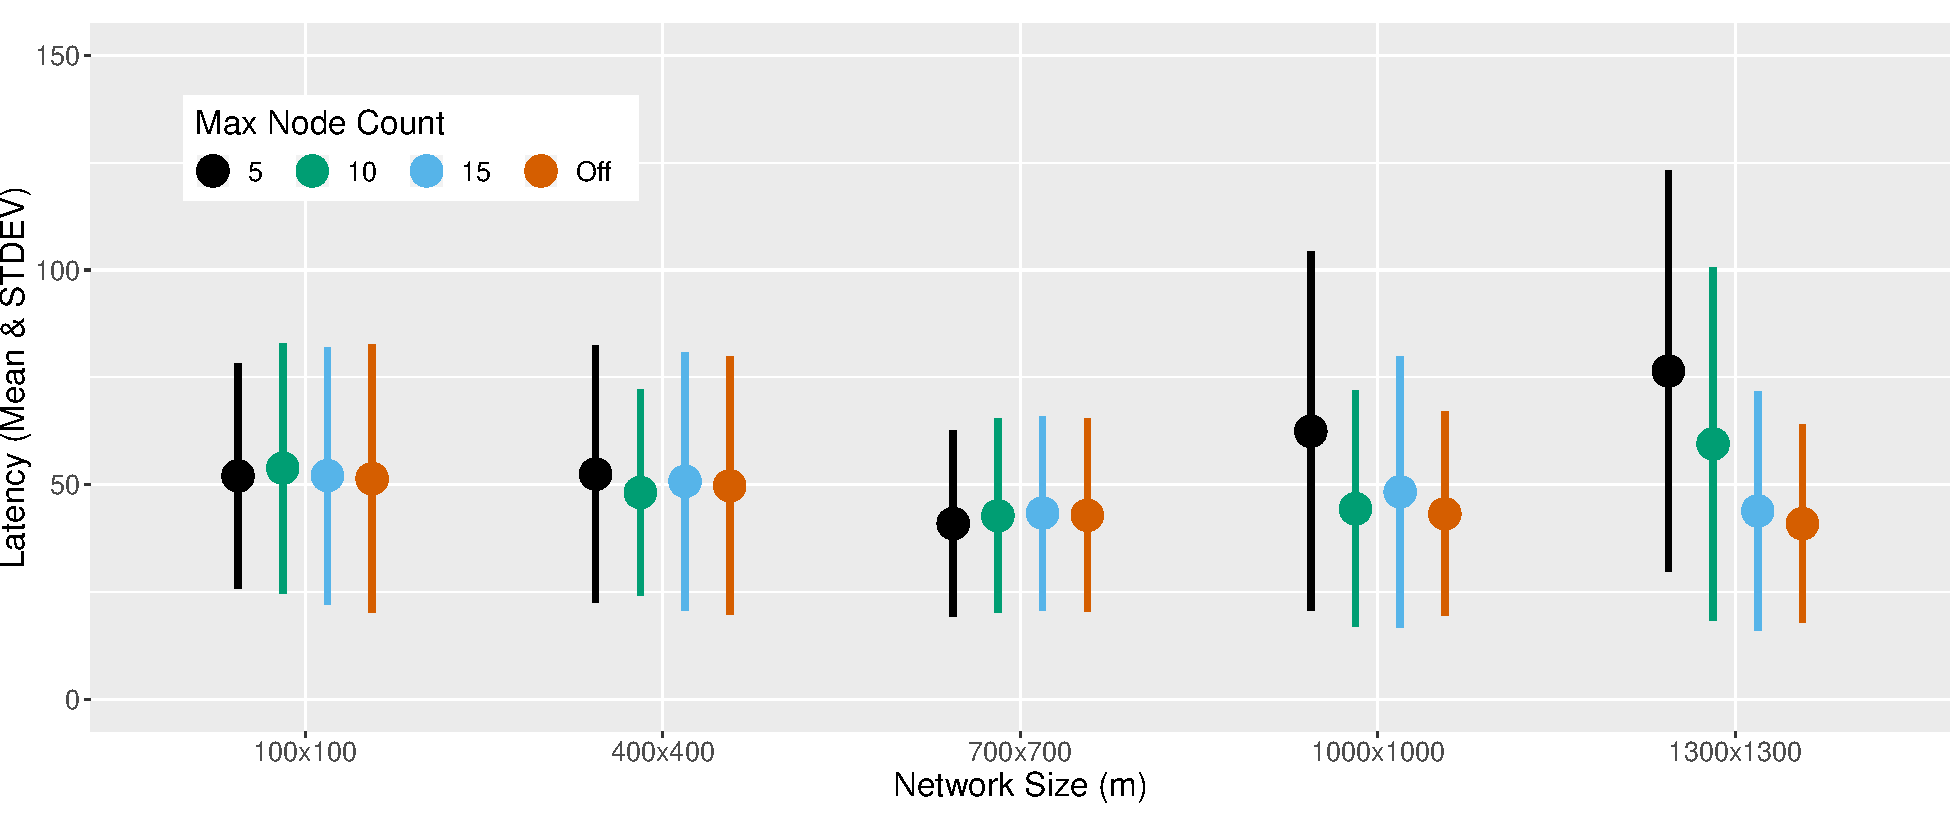
\includegraphics[width=\textwidth, keepaspectratio]{figure/Results/ParameterEvaluation/Latency/MaxNodeCount_Latency.pdf}
    \caption{Nodes per cluster ratio.}
    \label{subfig:max-node-count-latency}
\end{subfigure}

    \caption{The latency results for the parameter tests.}
    \label{fig:parameter-tests-latency}
\end{figure}

\chapter{Appendix 2}
\section{Parameter Values for the \atwo{} Comparison}
\label{app:parameter-values-for-the-atwo-comparison}
\begin{table}[H]
\centering
\caption{List of topologies with 50 nodes and the competition radius used for each topology.}
\label{tab:50-nodes-competition-radius-value}
\begin{tabular}{|r|l|l|l|l|}
\hline
\multicolumn{1}{|c|}{\textbf{Competition Radius}} & \multicolumn{4}{l|}{\textbf{Topologies}}                        \\ \hline
1                                                 & \multicolumn{4}{l|}{100x100, 400x400}                           \\ \hline
2                                                 & \multicolumn{4}{l|}{700x700, 1000x1000, 1300x1300}              \\ \hline
3                                                 & \multicolumn{4}{l|}{1600x1600, 1900x1900, 2200x2200, 2500x2500} \\ \hline
\end{tabular}
\end{table}

\begin{table}[H]
\centering
\caption{List of topologies with 200 nodes and the nodes per cluster ratio used for each topology.}
\label{tab:50-nodes-nodes-per-cluster-ratio-value}
\begin{tabular}{|r|l|}
\hline
\textbf{Nodes Per Cluster Ratio} & \textbf{Topologies}           \\ \hline
10                               & 100x100, 400x400              \\ \hline
30                               & 700x700, 1000x1000, 1300x1300 \\ \hline
\end{tabular}
\end{table}

%\chapter{Application Heat maps for Reliability Comparison}
%In these figures, x-axis represents rounds and therefore progression in time, each row on the y-axis represents one node. The colour of a cell indicates what application a node executed during that round.
%\begin{figure}[H]
    \centering
    \begin{subfigure}{\textwidth}
        \centering
        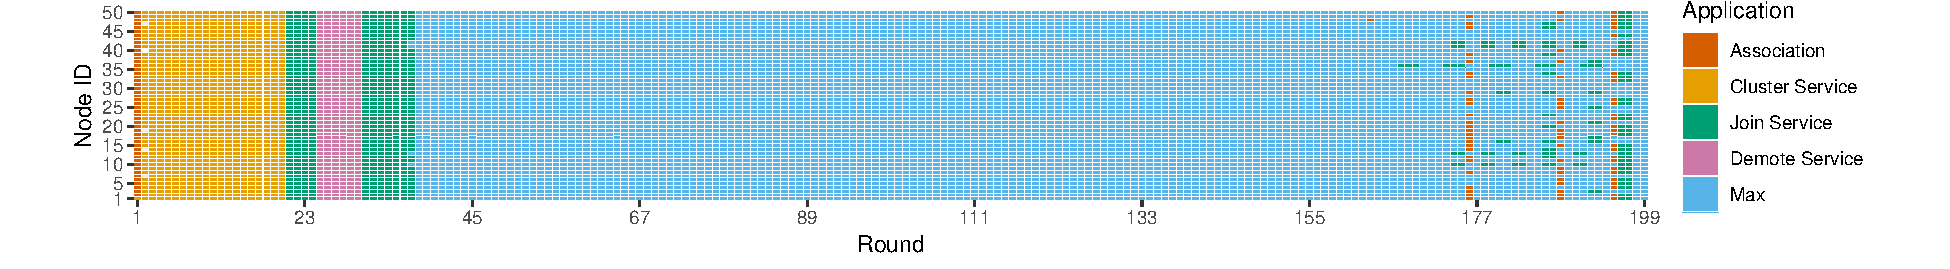
\includegraphics[width=\textwidth]{figure/Results/ReliabilityDiscussionApplicationHeatmaps/applicationmap50x50_1.pdf}
        \label{subfig:application-map-50-nodes-round-1-199}
    \end{subfigure}
    \hfill
    \begin{subfigure}{\textwidth}
        \centering
        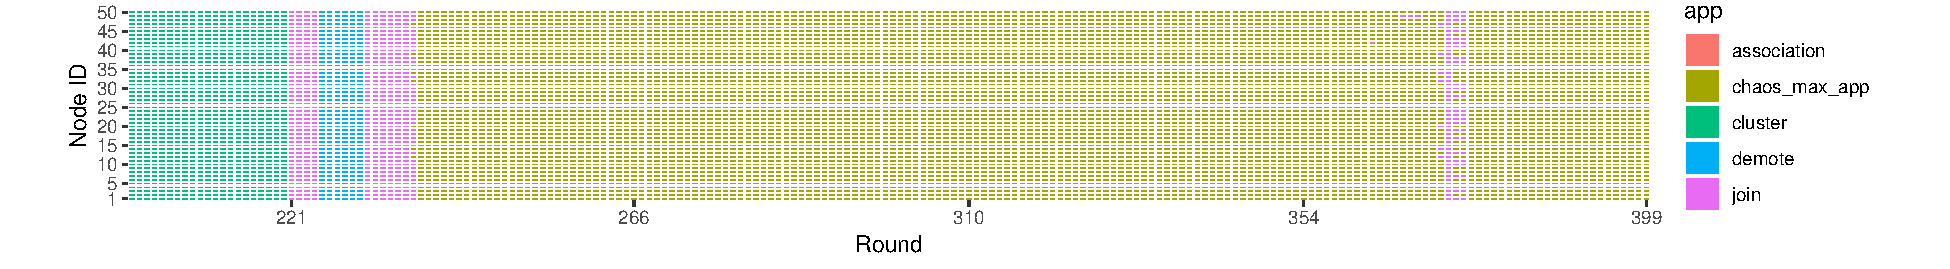
\includegraphics[width=\textwidth]{figure/Results/ReliabilityDiscussionApplicationHeatmaps/applicationmap50x50_2.pdf}
        \label{subfig:application-map-50-nodes-round-200-399}
    \end{subfigure}
    \begin{subfigure}{\textwidth}
        \centering
        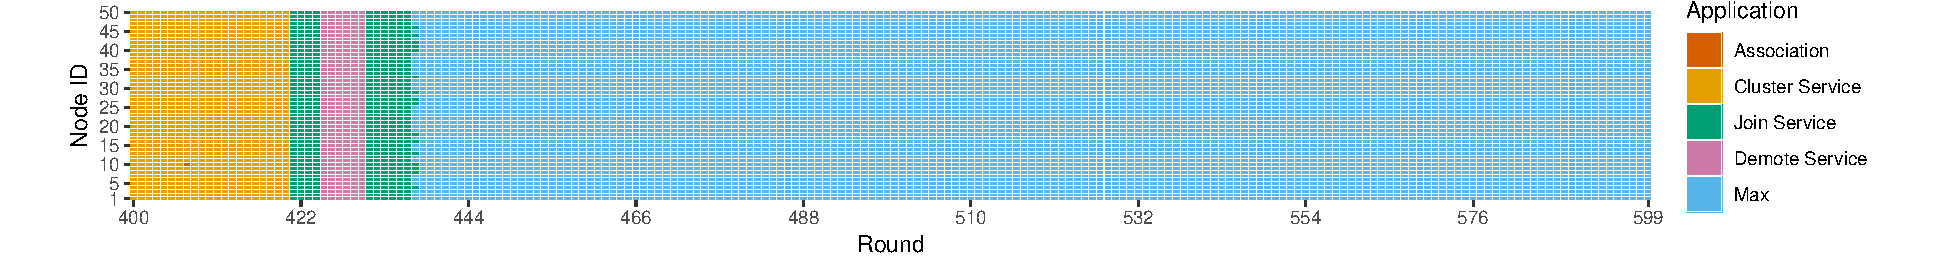
\includegraphics[width=\textwidth]{figure/Results/ReliabilityDiscussionApplicationHeatmaps/applicationmap50x50_3.pdf}
        \label{subfig:application-map-50-nodes-round-400-599}
    \end{subfigure}
    \caption{Application heat map of a test with 50 nodes over a 100x100 network area executing 600 rounds. Join is rarely executed outside its specified schedule.}
    \label{fig:application-map-50-nodes}
\end{figure}
%\begin{figure}[H]
\label{fig:application-map-200-nodes}
    \centering
    \begin{subfigure}{0.9\textwidth}
        \centering
        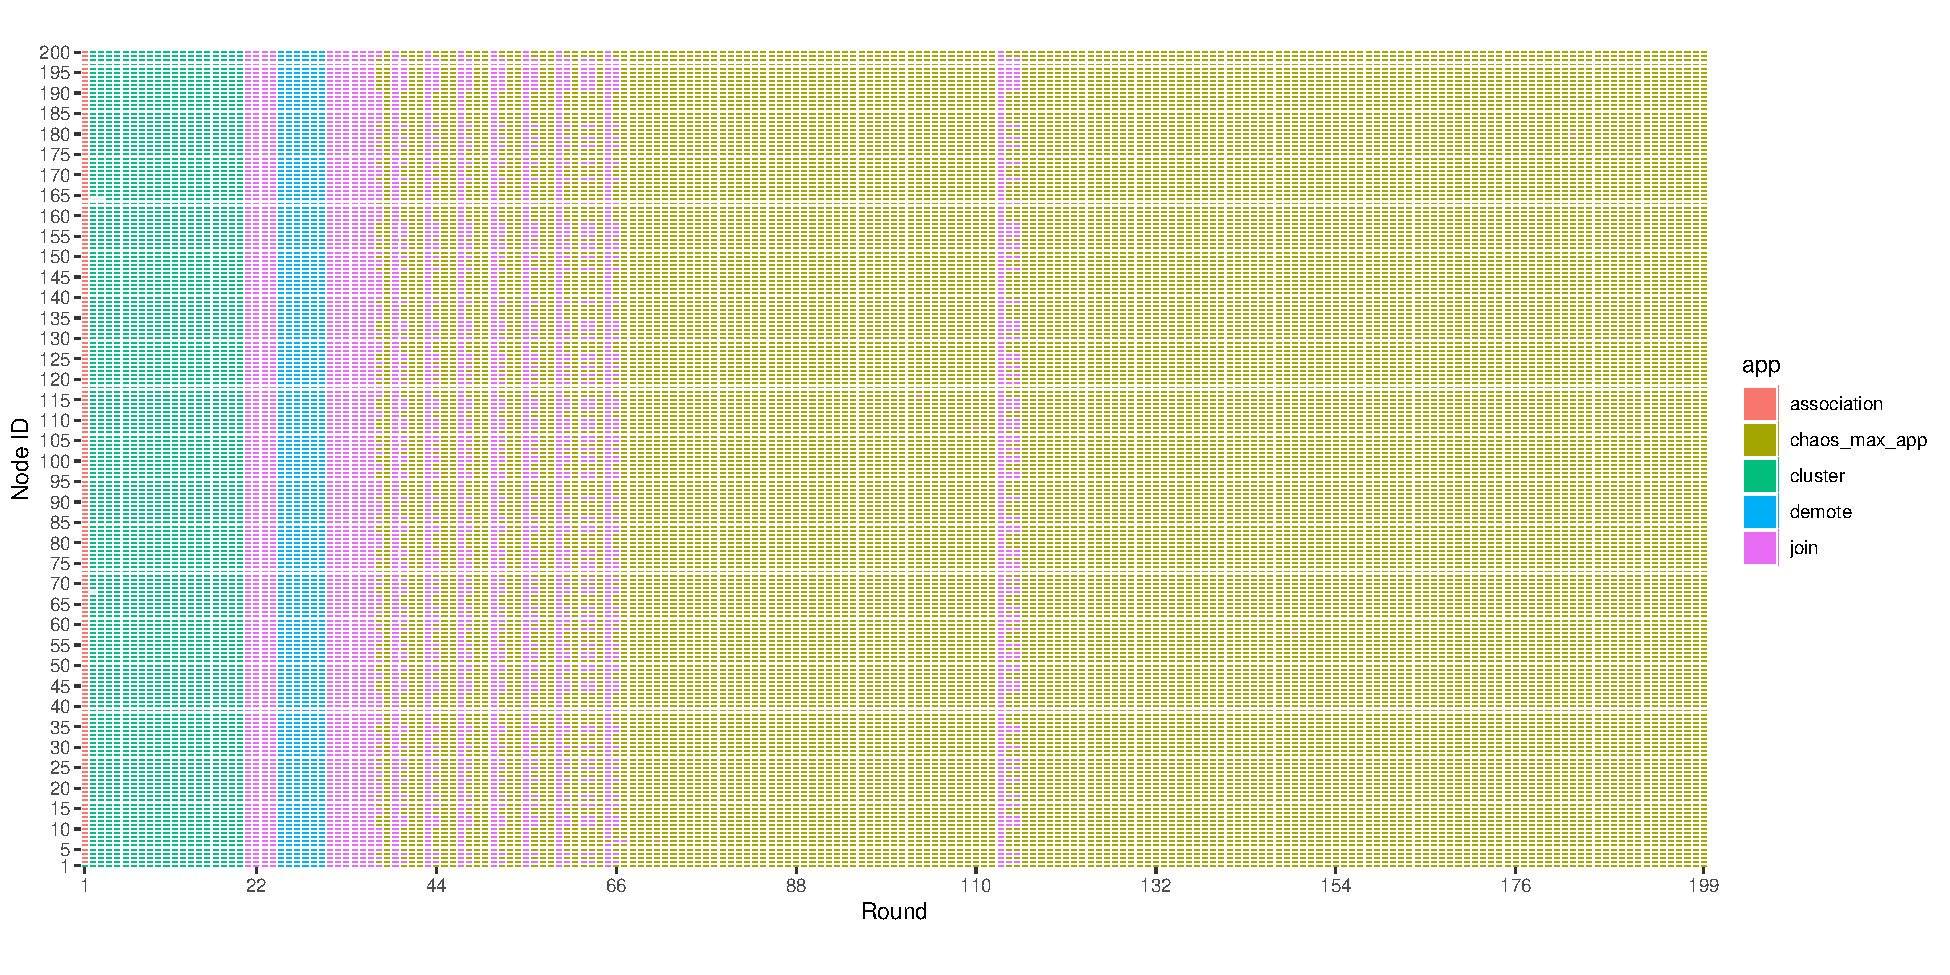
\includegraphics[width=\textwidth]{figure/Results/ReliabilityDiscussionApplicationHeatmaps/applicationmap200x200_1.pdf}
        \label{subfig:application-map-200-nodes-round-1-199}
    \end{subfigure}
    \hfill
    \begin{subfigure}{0.9\textwidth}
        \centering
        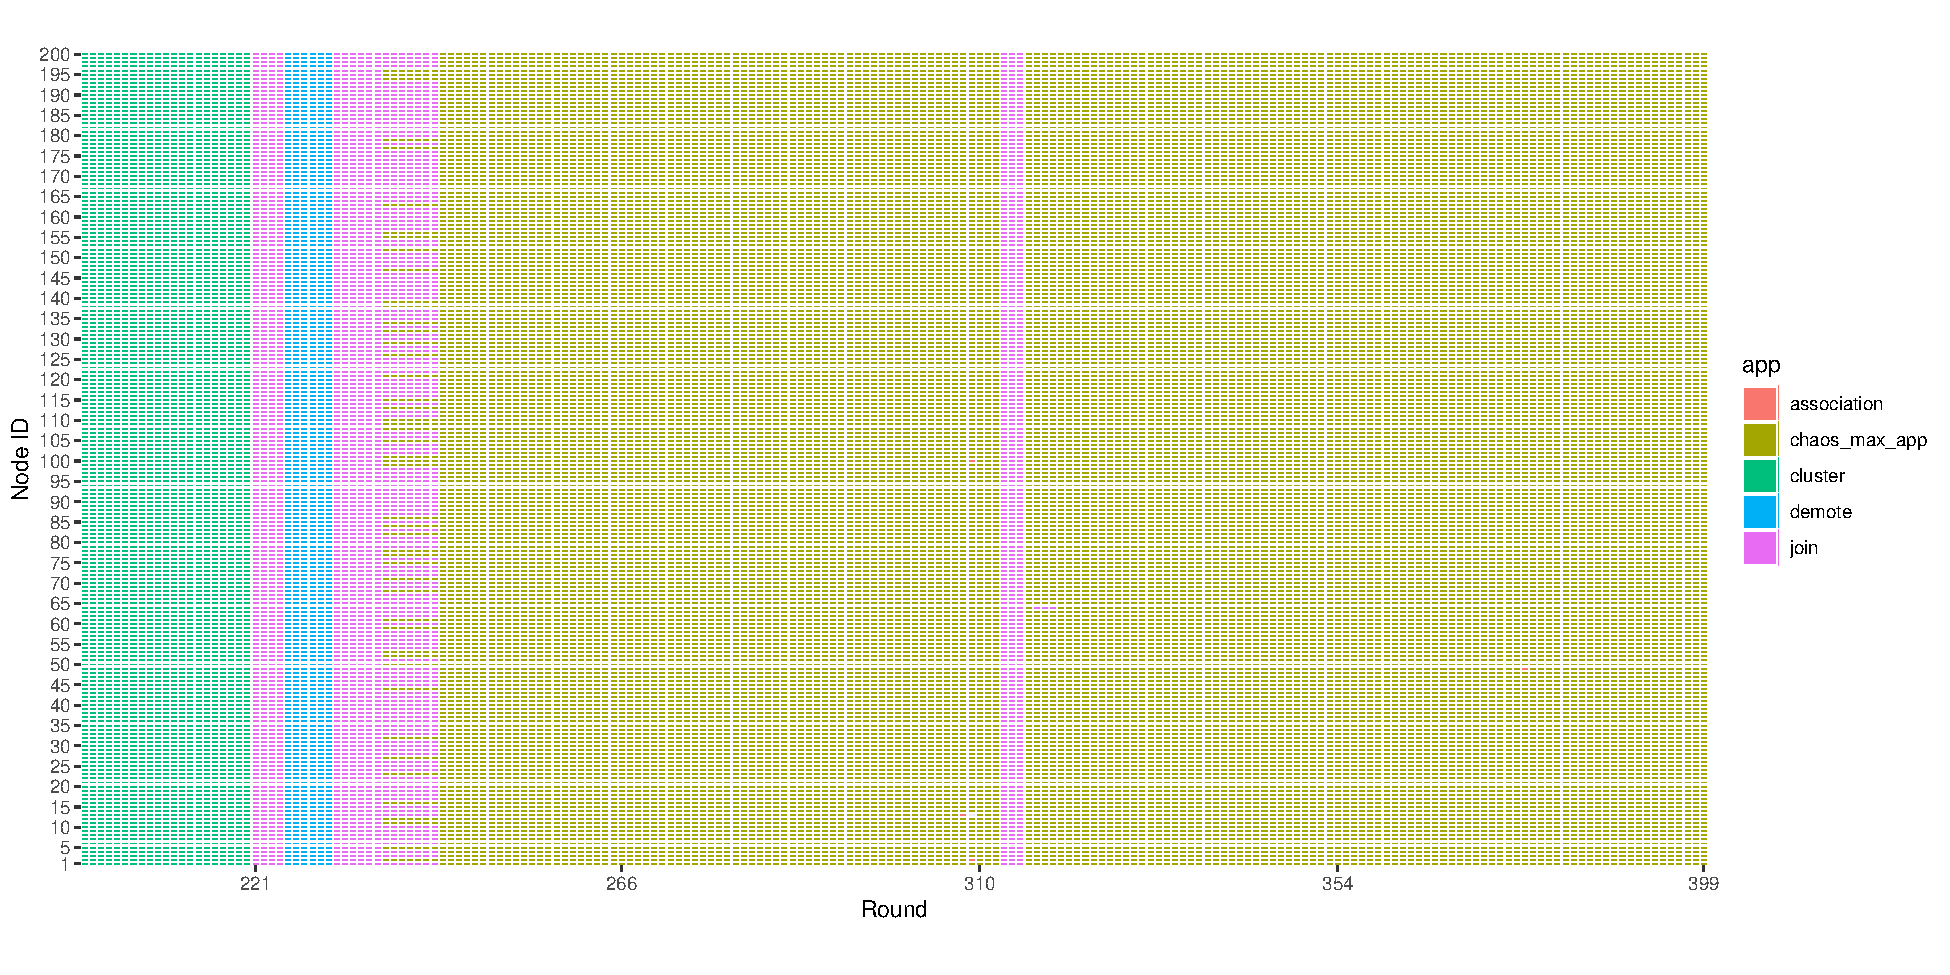
\includegraphics[width=\textwidth]{figure/Results/ReliabilityDiscussionApplicationHeatmaps/applicationmap200x200_2.pdf}
        \label{subfig:application-map-200-nodes-round-200-399}
    \end{subfigure}
    \begin{subfigure}{0.9\textwidth}
        \centering
        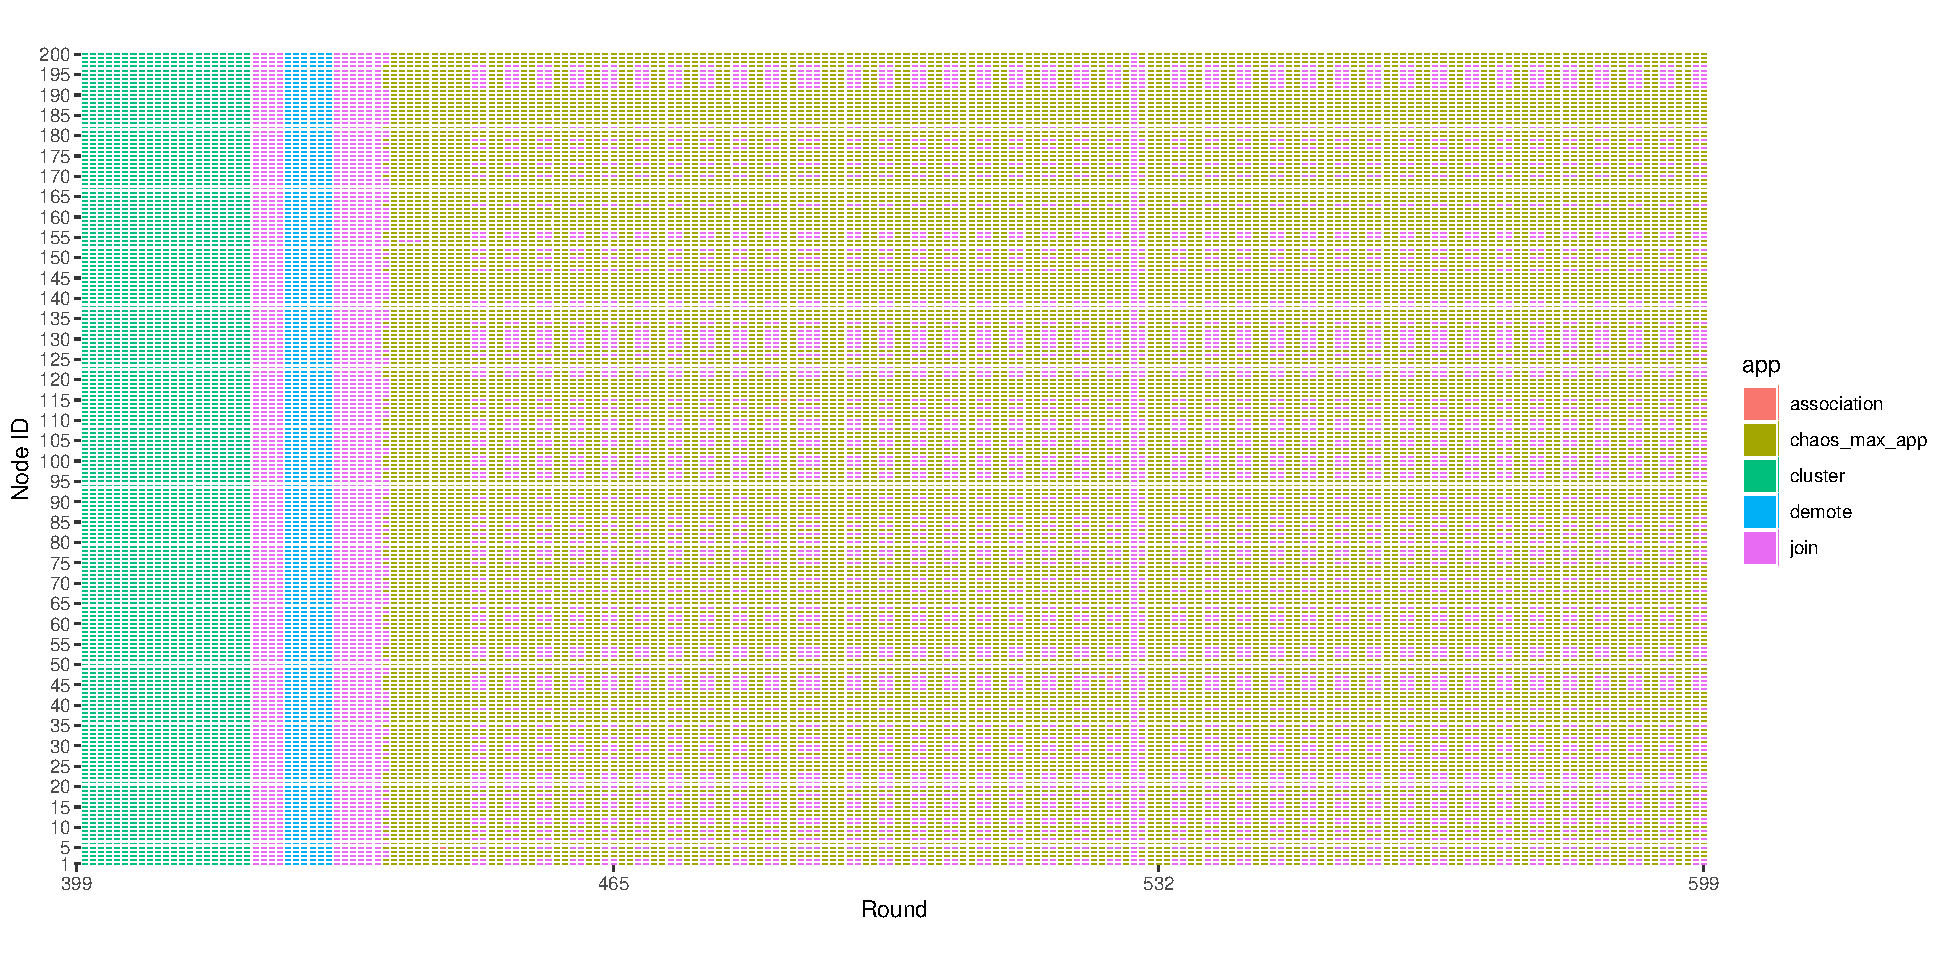
\includegraphics[width=\textwidth]{figure/Results/ReliabilityDiscussionApplicationHeatmaps/applicationmap200x200__3.pdf}
        \label{subfig:application-map-200-nodes-round-400-599}
    \end{subfigure}
    \caption{Application heat map of a test with 200 nodes over a 100x100 network area executing 600 rounds. Some clusters often execute join, especially after the last clustering occurring in rounds 400 to 437}
\end{figure}


\end{document}